%%
%% This is file `elsarticle-template-num.tex',
%% generated with the docstrip utility.
%%
%% The original source files were:
%%
%% elsarticle.dtx  (with options: `numtemplate')
%% 
%% Copyright 2007, 2008 Elsevier Ltd.
%% 
%% This file is part of the 'Elsarticle Bundle'.
%% -------------------------------------------
%% 
%% It may be distributed under the conditions of the LaTeX Project Public
%% License, either version 1.2 of this license or (at your option) any
%% later version.  The latest version of this license is in
%%    http://www.latex-project.org/lppl.txt
%% and version 1.2 or later is part of all distributions of LaTeX
%% version 1999/12/01 or later.
%% 
%% The list of all files belonging to the 'Elsarticle Bundle' is
%% given in the file `manifest.txt'.
%% 

%% Template article for Elsevier's document class `elsarticle'
%% with numbered style bibliographic references
%% SP 2008/03/01

%\documentclass[preprint,12pt]{elsarticle}
\documentclass[preprint,10pt]{elsarticle}
%\documentclass[final,3p,times]{elsarticle} 

%% Use the option review to obtain double line spacing
%% \documentclass[authoryear,preprint,review,12pt]{elsarticle}

%% Use the options 1p,twocolumn; 3p; 3p,twocolumn; 5p; or 5p,twocolumn
%% for a journal layout:
%% \documentclass[final,1p,times]{elsarticle}
%% \documentclass[final,1p,times,twocolumn]{elsarticle}
%% \documentclass[final,3p,times]{elsarticle}
%% \documentclass[final,3p,times,twocolumn]{elsarticle}
%% \documentclass[final,5p,times]{elsarticle}
%% \documentclass[final,5p,times,twocolumn]{elsarticle}

%% if you use PostScript figures in your article
%% use the graphics package for simple commands
\usepackage{float}
\usepackage{color}
\usepackage{caption}
\usepackage{subcaption}
\usepackage{appendix}
%% or use the graphicx package for more complicated commands
\usepackage{graphicx}
%% or use the epsfig package if you prefer to use the old commands
%% \usepackage{epsfig}

%% The amssymb package provides various useful mathematical symbols 
%% The amsthm package provides extended theorem environments
\usepackage{amssymb}
\usepackage{amsmath}
% more math
\usepackage{amsfonts}
\usepackage{amstext}
\usepackage{amsbsy}
\usepackage{mathbbol} 
%% The lineno packages adds line numbers. Start line numbering with
%% \begin{linenumbers}, end it with \end{linenumbers}. Or switch it on
%% for the whole article with \linenumbers.
\usepackage{lineno}
\usepackage{cancel}

\journal{Journal of Comp. Phys.}
%%%%%%%%%%%%%%%%%%%%%%%%%%%%%%%%%%%%%%%%%%%%%%%%%%%%%%%%%%%%%%%%%%%%
% operators
\renewcommand{\div}{\vec{\nabla}\! \cdot \!}
\newcommand{\grad}{\vec{\nabla}}
\newcommand{\divv}[1]{\vec{\nabla}^{#1}\! \cdot \!}
\newcommand{\gradd}[1]{\vec{\nabla}^{#1}}
% latex shortcuts
\newcommand{\bea}{\begin{eqnarray}}
\newcommand{\eea}{\end{eqnarray}}
\newcommand{\be}{\begin{equation}}
\newcommand{\ee}{\end{equation}}
\newcommand{\bal}{\begin{align}}
\newcommand{\eali}{\end{align}}
\newcommand{\bi}{\begin{itemize}}
\newcommand{\ei}{\end{itemize}}
\newcommand{\ben}{\begin{enumerate}}
\newcommand{\een}{\end{enumerate}}
% DGFEM commands
\newcommand{\jmp}[1]{[\![#1]\!]}                     % jump
\newcommand{\mvl}[1]{\{\!\!\{#1\}\!\!\}}             % mean value
\newcommand{\keff}{\ensuremath{k_{\textit{eff}}}\xspace}
% shortcut for domain notation
\newcommand{\D}{\mathcal{D}}
% vector shortcuts
\newcommand{\vo}{\vec{\Omega}}
\newcommand{\vr}{\vec{r}}
\newcommand{\vn}{\vec{n}}
\newcommand{\vnk}{\vec{\mathbf{n}}}
\newcommand{\vj}{\vec{J}}
\newcommand{\eig}[1]{\| #1 \|_2}

\newcommand{\EI}{\mathcal{E}_h^i}
\newcommand{\ED}{\mathcal{E}_h^{\partial \D^d}}
\newcommand{\EN}{\mathcal{E}_h^{\partial \D^n}}
\newcommand{\ER}{\mathcal{E}_h^{\partial \D^r}}
\newcommand{\reg}{\textit{reg}}

\newcommand{\norm}{\textrm{norm}}
\renewcommand{\Re}{\textrm{Re\,}}
\newcommand{\Pe}{\textrm{P\'e\,}}

\newcommand{\resi}{R_e}
%\newcommand{\resinew}{\tilde{D}_e}
\newcommand{\resinew}{\widetilde{\resi}}
\newcommand{\matder}[1]{\frac{\textrm{D} #1}{\textrm{D} t}}


% extra space
\newcommand{\qq}{\quad\quad}
% common reference commands
\newcommand{\eqt}[1]{Eq.~(\ref{#1})}                     % equation
\newcommand{\fig}[1]{Fig.~\ref{#1}}                      % figure
\newcommand{\tbl}[1]{Table~\ref{#1}}                     % table
\newcommand{\sct}[1]{Section~\ref{#1}}                   % section
\newcommand{\app}[1]{Appendix~\ref{#1}}                   % appendix

\newcommand\br{\mathbf{r}}
%\newcommand{\tf}{\varphi}
\newcommand{\tf}{b}

\newcommand{\tcr}[1]{\textcolor{red}{#1}}
\newcommand{\tcb}[1]{\textcolor{blue}{#1}}
\newcommand{\mt}[1]{\marginpar{ {\tiny \tcr{#1} }}}

\newtheorem{remark}{Remark}

\bibliographystyle{elsarticle-num}
%%%%%%%%%%%%%%%%%%%%%%%%%%%%%%%%%%%%%%%%%%%%%%%%%%%%%%%%%%%%%%%%%%%%%
%
%   BEGIN DOCUMENT
%
%%%%%%%%%%%%%%%%%%%%%%%%%%%%%%%%%%%%%%%%%%%%%%%%%%%%%%%%%%%%%%%%%%%%%
\begin{document}

%%%%%%%%%%%%%%%%%%%%%%%%%%%%%%%%%%%%%%%%%%%%%%%%%%%%%%%%%%%%%%%%%%%%
\begin{frontmatter}

%% Title, authors and addresses

%% use the tnoteref command within \title for footnotes;
%% use the tnotetext command for theassociated footnote;
%% use the fnref command within \author or \address for footnotes;
%% use the fntext command for theassociated footnote;
%% use the corref command within \author for corresponding author footnotes;
%% use the cortext command for theassociated footnote;
%% use the ead command for the email address,
%% and the form \ead[url] for the home page:
%\title{Title\tnoteref{label1}}
%% \tnotetext[label1]{}
%% \author{Name\corref{cor1}\fnref{label2}}
%% \ead{email address}
%% \ead[url]{home page}
%% \fntext[label2]{}
%% \cortext[cor1]{}
%% \address{Address\fnref{label3}}
%% \fntext[label3]{}
%-------------------------
%-------------------------
%\title{Extension of the entropy viscosity method to the low Mach regime for the multi-dimensional Euler equations\\
\title{Entropy-based viscous regularization for the multi-dimensional Euler equations in low-Mach and transonic flows}
%-------------------------
%-------------------------
\author{Marc O. Delchini\fnref{label1}}
\ead{delchmo@tamu.edu}

\author{Jean C. Ragusa\corref{cor1}\fnref{label1}}
\ead{jean.ragusa@tamu.edu}

\author{Ray A. Berry\fnref{label2}}
\ead{ray.berry@inl.gov}

\address[label1]{Department of Nuclear Engineering, Texas A\&M University, College Station, TX 77843, USA \fnref{label1}}

\address[label2]{Idaho National Laboratory, Idaho Falls, ID 83415, USA \fnref{label2}}

\cortext[cor1]{Corresponding author}
%-------------------------
%-------------------------
%-------------------------
\begin{abstract}
The entropy viscosity method, introduced by Guermond et al. \cite{jlg1, jlg2}, is extended to the multi-dimensional Euler equations for both subsonic (very low Mach numbers) and supersonic flows. 
We show that the current definition of the viscosity coefficients \cite{jlg1, jlg2} is not adapted to low-Mach flows and we provide a robust alternate definition valid for any Mach number value. The new definitions are derived from a low-Mach asymptotic study. 
In addition, the entropy minimum principle is used to derive the viscous regularization terms for Euler equations with variable area for nozzle flow problems. 
Various 1-D and 2-D numerical tests are presented : flow in a convergent-divergent nozzle, Leblanc shock tube, slow moving shock, strong shock for liquid phase, subsonic flow around a 2-D cylinder and over a circular hump, and supersonic flow in a compression corner. Convergence studies are performed using analytical solutions in 1-D. 
The ideal gas and stiffened gas equations of state are employed. The Stiffened gas equation of state can be used for both gas and liquid phases \cite{SGEOS}.\tcr{is there a better name, that would let the reader understand this is for liquid as well?} \tcb{Is this ok?}
\end{abstract}
%-------------------------
%-------------------------
\begin{keyword}
  entropy viscosity method \sep viscous stabilization method \sep low-Mach regime \sep shocks \sep Euler equations with variable area .
\end{keyword}
%-------------------------
\end{frontmatter}
%%%%%%%%%%%%%%%%%%%%%%%%%%%%%%%%%%%%%%%%%%%%%%%%%%%%%%%%%%%%%%%%%%%%
\linenumbers
%%%%%%%%%%%%%%%%%%%%%%%%%%%%%%%%%%%%%%%%%%%%%%%%%%%%%%%%%%%%%%%%%%%%%%%%%%%%%%%%%%%%%%%%%%%%%%%%%%%%
%%%%%%%%%%%%%%%%%%%%%%%%%%%%%%%%%%%%%%%%%%%%%%%%%%%%%%%%%%%%%%%%%%%%%%%%%%%%%%%%%%%%%%%%%%%%%%%%%%%%
\section{Introduction} \label{sec:intro}
%%%%%%%%%%%%%%%%%%%%%%%%%%%%%%%%%%%%%%%%%%%%%%%%%%%%%%%%%%%%%%%%%%%%%%%%%%%%%%%%%%%%%%%%%%%%%%%%%%%%
%%%%%%%%%%%%%%%%%%%%%%%%%%%%%%%%%%%%%%%%%%%%%%%%%%%%%%%%%%%%%%%%%%%%%%%%%%%%%%%%%%%%%%%%%%%%%%%%%%%%
%\tcr{I think we should focus the introduction more}
%
%Incompressible flows are a particular case of compressible ones and therefore in principle, a
%compressible flow solver should be able to compute these flows. Unfortunately, there are experimental
%evidences showing that on a fixed mesh, the solutions of the compressible flow discretized
%equations are not an accurate approximation of the solutions of the incompressible model (e.g. see
%[29]). A first analysis of this problem appeared in [23] and this question has drawn a considerable
%attention [1–3,7,9,26,28,30] in the recent past. Several works have tried to explain the reasons of
%this difficulty and to construct numerical schemes valid for all Mach numbers. Some of these
%works extend to the compressible regime the numerical methods used for the computation of
%incompressible flows. Examples of these type of methods are for instance [1] or [30]. Another
%approaches rely on some modifications of high order shock capturing techniques. These approaches
%are for instance described in [2,7,22] for Roe discretization, in [3] for the HLLE scheme
%and in [28] for Flux schemes. Their principal ingredient is the use of preconditioning techniques
%originally developed for steady state computations [4,21,23] that are here selectively applied only
%to the upwind artificial viscosity.
%
%
%The efficient simulation of low Mach number flows is a subject of ongoing discussion in the
%CFD community. While the flow is expected to be incompressible, in a lot of applications
%the Mach number or the compressibility properties vary strongly in time or space. This is
%for example the case in nozzle  flow, chemically reacting flows or laminar combustion. It is
%well known that purely compressible flow solvers which were developed for transonic 
%flow produce wrong results at low Mach numbers. On the other hand, standard incompressible 
%flow solvers cannot deal with strong temperature or strong density gradients. This sets a
%demand for codes that can deal with flows at all Mach numbers.
%
%It is well known that it is difficult to solve the compressible equations for low Mach numbers.
%For an explicit scheme this is easily seen by looking at the time steps. For stability the time
%step must be chosen inversely proportional to the largest eigenvalue of the system which is
%approximately the speed of sound, c, for slow flows. However, other waves are convected at the
%fluid speed, u, which is much slower. Hence, these waves don’t change very much over a time
%step. Thus, thousands of time steps are required to reach a steady state. Should one try a
%multigrid acceleration one finds that the same disparity in wave speeds slows down the
%multigrid acceleration. With an implicit method an AD1 factorization is usually used so that
%one can easily invert the implicit factors. The use of AD1 introduces factorization errors which
%again slow down the convergence rate when there are wave speeds of very different magnitudes
%For small Mach numbers it can be shown [28,31] that the incompressible equations approximate
%the compressible equations. Hence, one needs to justify the use of the compressible
%equations for low Mach flows. We present several reasons why one would still use the
%compressible equations even though the Mach number of the flow is small.
%l There are many sophisticated compressible codes available that could be used for such
%problems especially in complicated geometries.
%l For low speed aerodynamic problems at a high angle of attack most of the flow consists of
%a low Mach number flow. However, there are localized regions containing shocks.
%l In many problems thermal effects are important and the energy equation is coupled to the
%other equations.
%
%The incompressible limit of a compressible flow is rather subtle due to the fact that the propagation rate of
%the pressure waves becomes infinite and the equations change their type. Within this limit the pressure splits up
%into a thermodynamic pressure term and a hydrodynamic pressure term. If the limit solution has constant
%temperature and density and if the boundary values satisfy the incompressibility constraint, then the
%thermodynamic pressure becomes the background pressure being constant in space and time. The hydrodynamic
%pressure appears in the incompressible equations as a sort of a Lagrangian multiplier with no connection
%to the equation of state. The asymptotic analysis of Klainerman and Majda in [9,10] gives insight into this
%limit behavior. They gave a mathematically rigorous derivation in the isentropic case. The asymptotic analysis
%was formally extended by Klein to the non-isentropic case and to multiple space scales in [11] in which he also
%gave an overview about other asymptotic considerations in this low Mach number regime. A detailed discussion
%of the incompressible limit is also given in the book of Wesseling [20].
%Numerical methods for the compressible equations may have difficulties with the zero Mach number limit
%because in the limit the speed of sound waves becomes infinite compared to the flow speed and thus leads to an
%elliptic coupling of pressure and velocity. Hence, all explicit numerical schemes become quite inefficient in the
%low Mach number regime due to their stability restriction (CFL condition). The other difficulty is that the
%pressure in the compressible equations converges to the thermodynamic pressure, which becomes the constant
%background pressure in the incompressible limit. This is the way how the equation of state for compressible
%flow is automatically satisfied and does not appear in the incompressible equations. For the compressible
%equations Bijl and Wesseling [2] introduced a splitting of the pressure into a thermodynamic and a hydrodynamic
%pressure term. Then they proposed an implicit numerical method that remains stable without reference
%to the sound velocity and which approximates the incompressible equations for Mach number zero. The constant
%thermodynamic pressure satisfies the equation of state and the hydrodynamic pressure serves as a
%Lagrangian multiplier to get the divergence-free property of the velocity. A formulation in conservative variables
%was later given in [18,20]. Similar to this approach Klein and Munz [12] and Munz et al. [13] proposed
%the multiple pressure variable (MPV) method based on the asymptotic results of Klein [11].

\tcr{above are good snippets from some papers.}

Over the past years an increasing interest raised for computational methods that can solve both compressible and incompressible flows. In engineering applications, there is often the need to solve for complex flows where a near incompressible regime or low Mach flow coexists with a supersonic flow domain. For example, such flow are encountered in aerodynamic in the study of airships. In the nuclear industry, flows are nearly the incompressible regime but compressible effects cannot be neglected because of the heat source and thus needs to be accurately resolved. \\
When solving the multi-D Euler equations for a wide range of Mach numbers, multiple problems have to address: stability, accuracy and acceleration of the convergence in the low Mach regime. Because of the hyperbolic nature of the equations, shocks can form during transonic and supersonic flows, and require the use of the numerical methods in order to stabilize the scheme and correctly resolve the discontinuities. The literature offers a wide range of stabilization methods: flux-limiter \cite{FluxLimiter, FluxLimiter2}, pressure-based viscosity method (\cite{PBV_book}), Lapidus method (\cite{Lapidus_paper, LMP, Lapidus_book}), and the entropy-viscosity method(\cite{jlg1, jlg2}) among others. These numerical methods are usually developed using simple equation of states and tested for transonic and supersonic flows where the disparity between the acoustic waves and the fluid speed is not large since the Mach number is of order one. This approach leads to a well-known accuracy problem in the low Mach regime where the fluid velocity is smaller that the speed of sound by multiple order of magnitude. The numerical dissipative terms become ill-scaled in the low Mach regime and lead to the wrong numerical solution by changing the nature of the equations solved. This behavior is well documented in the literature \cite{LowMach1, LowMach2, LowMach3} and often treated by performing a low Mach asymptotic study of the multi-D Euler equation. This method was originally used \cite{LowMach1} to show convergence of the compressible multi-D Euler equations to the incompressible ones. Thus, by using the same method, the effect of the dissipative terms in the low Mach regime, can be understood and, when needed, a fix is developed in order to ensure the convergence of the equations to the correct physical solution. This approach was used as a fixing method for multiple well known stabilization methods alike Roe scheme (\cite{Roe}) and SUPG \cite{LowMach3} while preserving the original stabilization properties of shocks.  \\
We propose, through this paper, to investigate how the entropy viscosity method, when applied to the multi-D Euler equations with variable area, behaves in the low Mach regime. This method was initially introduced by Guermond et al. to solve for the hyperbolic systems and has shown good results when used for solving the multi-D Euler equations with various discretization schemes. More importantly, it is simple to implement, can be used with unstructured grids,  and its dissipative terms are consistent with the entropy minimum principle and proven valid for any equation of state under certain conditions \cite{jlg}. \\
This paper is organized as follows: in \sct{sec:entro_visc} the current definition of the entropy viscosity method is recalled, and inconsistency with the low Mach regime are pointed out. Since our interest is in the variable area version of the multi-D Euler equation, the reader is guided trough the steps leading to the derivation of the dissipative terms on the model of \cite{jlg}. Then in \sct{sec:extension}, a new definition of the viscosity coefficient is introduced and derived from a low Mach asymptotic study. After detailing the spatial and temporal discretization method in \sct{sec:solution_tech}, 1-D and 2-D numerical results are presented in \sct{sec:results} for a wide range of Mach numbers: low Mach flow over a cylinder and a circular bump, and supersonic flow in a compression corner \cite{CompressionCorner}. Convergence studies are performed in 1-D, in order to demonstrate the accuracy of the solution. \\
\tcr{I wouldn't recall this here. Let me think about that.}\\
For purpose of clarity, the multi-D Euler equations with variable area are recalled in \eqt{eq:euler_eq} and the corresponding variables are defined:
%
\begin{equation}
\label{eq:euler_eq}
\left\{ 
\begin{array}{lll}
\partial_t \left( \rho A\right) + \div \left( \rho \vec{u} A\right) = 0\\
\partial_t \left( \rho \vec{u} A\right) + \div \left[ \left( \rho \vec{u} \otimes \vec{u} + P \mathbf{I} \right) A \right] = P \grad A\\
\partial_t \left( \rho E A\right) + \div \left[ \vec{u} \left( \rho E + P \right) A\right] = 0 \\
P = P\left( \rho, e \right)
\end{array}
\right.
\end{equation}
%
where $\rho$, $\rho \vec{u}$ and $\rho E$ are the density, the momentum and the total energy, respectively, and will be referred to as the conservative variables. The pressure $P$ is computed with an equation of state expressed in function of the density $\rho$ and the specific internal energy $e$. The tensor product $\vec{a} \otimes \vec{b}$ is taken with the following convention: $(\vec{a} \otimes \vec{b})_{i,j} = a_i b_j$. Lastly, the terms $\partial_t$, $\grad$, $\div$ and $\mathbf{I}$ denote the temporal derivative, the gradient and divergent operators, and the identity tensor, respectively. The variable area $A$ is assumed spatial dependent.

%%%%%%%%%%%%%%%%%%%%%%%%%%%%%%%%%%%%%%%%%%%%%%%%%%%%%%%%%%%%%%%%%%%%%%%%%%%%%%%%%%%%%%%%%%%%%%%%%%%%
%%%%%%%%%%%%%%%%%%%%%%%%%%%%%%%%%%%%%%%%%%%%%%%%%%%%%%%%%%%%%%%%%%%%%%%%%%%%%%%%%%%%%%%%%%%%%%%%%%%%
\section{The Entropy Viscosity Method} \label{sec:entro_visc}
%%%%%%%%%%%%%%%%%%%%%%%%%%%%%%%%%%%%%%%%%%%%%%%%%%%%%%%%%%%%%%%%%%%%%%%%%%%%%%%%%%%%%%%%%%%%%%%%%%%%
%%%%%%%%%%%%%%%%%%%%%%%%%%%%%%%%%%%%%%%%%%%%%%%%%%%%%%%%%%%%%%%%%%%%%%%%%%%%%%%%%%%%%%%%%%%%%%%%%%%%

%===================================================================================================
\subsection{Background} \label{sec:background}
%===================================================================================================
In this section, the entropy viscosity method \cite{jlg1, jlg2, jlg3, valentin} is recalled for the multi-D Euler equations (with constant area $A$). The method consists of adding dissipative terms with a viscosity coefficient modulated by the entropy production; this allows for a high-order accuracy when the solution is smooth (provided that the spatial and temporal discretizations also are high order). 
The derivation of the viscous regularization (dissipative terms) is carried out to be consistent with the entropy minimum principle theorem; details of the derivation and proofs can be found in \cite{jlg}. The viscous regularization obtained is valid for any equation of state as long as the physical entropy function $s$ is such that $-s$ is a convex function with respect to the internal energy $e$ and the specific volume $1/\rho$. Euler equations with viscous regularization are recalled in \eqt{eq:euler_visc}:
\begin{subequations}
\label{eq:euler_visc}
%
\begin{equation}
\partial_t \rho  + \div \left( \rho \vec{u} \right) = \div \left( \kappa \grad \rho \right) 
\end{equation}
%
\begin{equation}
\partial_t \left( \rho \vec{u} \right) + \div \left( \rho \vec{u} \otimes \vec{u} + P \mathbf{I} \right) = \div \left( \mu \rho \grad^s \vec{u}  + \kappa \vec{u} \otimes \grad \rho \right)  
\end{equation}
%
\begin{equation}
\partial_t \left( \rho E \right) + \div \left[ \vec{u} \left( \rho E + P \right) \right] = \div \left( \kappa \grad \left( \rho e \right) + \frac{1}{2}|| \vec{u} ||^2 \kappa \grad \rho +  \rho \mu \vec{u} \grad \vec{u}  \right) 
\end{equation}
\end{subequations}
%
where $\kappa$ and $\mu$ are positive viscosity coefficients. $\grad^s \vec{u}$ denotes the symmetric gradient operator that guarantees the method to be rotationally invariant \cite{jlg}.

The viscous regularization (\eqt{eq:euler_visc}) requires the numerical computation of viscosity coefficients. Many stabilization approaches have been proposed in the literature such as the Lapidus (pressure-based) method \cite{Lapidus_book, Lapidus_paper}. Here, we follow the work of Guermond et al. and define the viscosity coefficients, $\kappa$ and $\mu$, based on the local entropy production. These coefficients are evaluated using the local entropy residual $\resi(\vec{r},t)$ defined in \eqt{eq:ent_residual}; $\resi(\vec{r},t)$ is known to be peaked in shocks and vanishingly small elsewhere \cite{Toro}. 
%
\begin{equation}
\label{eq:ent_residual}
\resi(\vec{r}, t) := \partial_t s + \vec{u} \cdot \grad s
\end{equation}
%
In the current version of the method, the ratio of $\kappa$ to $\mu$ is defined as a numerical Prandlt number, $Pr$, that has to be supplied. Since $\resi(\vec{r},t)$ can be extremely larger in shocks, the definition of the viscosity also includes a first-order viscosity coefficient that serves as upper bound for the entropy-based viscosity coefficients. The first-order viscosity coefficients, denoted by $\mu_{\max}$ and $\kappa_{\max}$, are chosen so that the numerical scheme becomes equivalent to the upwind scheme when the first-order coefficients are employed. The upwind scheme is known to be over-dissipative but guarantees monotonicity \cite{Toro}. In practice, the viscosity coefficients only saturate to the first-order viscosity coefficients in shocks and are much smaller elsewhere, hence avoiding over-dissipation due tot he upwind method.  The first-order viscosity coefficients $\mu_{\max}$ and $\kappa_{\max}$ are equal and set proportional to the local largest eigenvalue $|| \vec{u} || + c $:
%
\begin{equation}
\label{eq:fo}
\mu_{\max}(\vec{r}, t) = \kappa_{\max}(\vec{r}, t) = \frac{h}{2} \left( || \vec{u}(\vec{t,r}) || + c(\vec{t,r}) \right),
\end{equation}
%
where $h$ is the local grid size (for higher than linear finite element representations, $h$ is defined as the ratio of the grid size to the polynomial order of the test functions used, see Eq. 2.4 in \cite{valentin}). For simplicity, the first-order viscosity will be referred to as the $\kappa_{\max}(\vec{r}, t)$. In practice, the quantities are evaluated within a given cell $K$ at quadrature points:
%
\begin{equation}
\label{eq:fo_quad}
\kappa^K_{\max}(\vec{r}_q, t) = \frac{h_K}{2} \left( || \vec{u}(\vec{t,r_q}) || + c(\vec{t,r_q}) \right),
\end{equation}
%
where $\vec{r}_q$ denotes the position of a quadrature point.\\
As stated earlier, the entropy viscosity coefficients, denoted by $\kappa_e$ and $\mu_e$, are set proportional to the entropy production evaluated by computing the local entropy residual $\resi$. The definitions also include the inter-element jump of the entropy flux $J$, thus allowing for the detection of discontinuities other than shocks:
%
\begin{eqnarray}
\label{eq:ent_visc_coeff}
\mu^K_e(\vec{r}_q,t) &=&  h_K^2 \frac{\max\left( | \resi^K(\vec{r}_q,t) |, J^K[s](t) \right)}{|| s - \bar{s} ||_\infty}  \nonumber \\
\kappa^K_e(\vec{r}_q,t) &=& Pr \cdot \mu^K_e(\vec{r}_q,t)
\end{eqnarray}
%
where $|| \cdot ||_\infty$ and $\bar{\cdot}$ denote the $L_\infty$-norm and the average operator over the entire computational domain, respectively. The definition of the entropy jump $J[s]$ is spatial discretization-dependent and examples of definitions can be found in \cite{valentin} for DGFEM. For continuous FEM, the jump of a given quantity is defined as the inter-element change in its normal derivative ($\partial_n = \grad \cdot \vec{n}$) along the common face separating the two elements. We take the largest value over all faces $f$ present on the boundary $\partial K$ of element $K$:
%
\begin{equation}
\label{eq:jump_CFEM}
J^K[s](t) = \max_{f\in\partial K}  \max_{\vec{r}_q \in f} \jmp{\grad s(\vec{r}_q,t) \cdot \vec{n}(\vec{r}_q) }_f
\end{equation}
%
where $\jmp{a(\vec{r}_q)}_f$ denotes the inter-element jump in $a(\vec{r})$ at quadrature point $\vec{r}_q$ on face $f$.  
The denominator $|| s - \bar{s} ||_\infty$ is used for dimensionality purposes \tcr{and should not be of the same order as $h$, on penalty of loosing the high-order accuracy} \tcb{you do not like this?}. Currently, there are no theoretical justification for choosing the denominator. 
Finally, the viscosity coefficients $\mu$ and $\kappa$ are as follows:
%
\begin{equation}
\mu(\vec{r},t)    = \min\Big( \mu_e(\vec{r},t)   \,,\, \mu_{\max}(\vec{r},t)    \Big) 
\quad \text{ and } \quad 
\kappa(\vec{r},t) = \min\Big( \kappa_e(\vec{r},t)\,,\, \kappa_{\max}(\vec{r},t) \Big).
\end{equation}
%
These definitions enable the following properties: 
In shock regions, the entropy viscosity coefficient will experience a peak because of entropy production and thus will saturates to the first-order viscosity. The first-order coefficients are known to be over-dissipative and will smooth out any oscillatory behavior. Elsewhere in the domain, entropy production will be small and the viscosity coefficients $\mu$ and $\kappa$ are small and of order $h^2$.
Using the above definitions, high-order accuracy for the entropy-based viscous stabilization method was demonstrated using several 1-D shock tube and various 2-D tests \cite{jlg1, jlg2, valentin}.

%===================================================================================================
\subsection{Issues in the Low-Mach Regime} 
%===================================================================================================

In the Low-Mach Regime, the flow is known to be isentropic, resulting in very little entropy production. Since the entropy viscosity method is directly based on the evaluation of the local entropy production, it is of interest to study how the entropy viscosity coefficients $\mu$ and $\kappa$ scale in the low-Mach regime. In practice, the entropy residual $\resi$ will be very small in that regime and so will be the denominator $|| s - \bar{s} ||_\infty$, thus making the definition of the viscosity coefficients in \eqt{eq:ent_visc_coeff} undetermined and likely ill-scaled.  One possible rigorous approach would consist of expanding the numerator and denominator in terms of the Mach number and deriving its limit when the Mach number goes to zero. Such derivation may not be staightforward, especially for general equations of state; however, this can be avoided by noticing that the entropy residual $\resi$ can be recast as a function of pressure, density, velocity, and speed of sound as shown in \eqt{eq:ent_res} of \sct{sec:new_ent_prod}. This alternate entropy residual definition is the basis for the low-Mach analysis carried out in this paper and possesses several advantages that are detailed in \sct{sec:new_ent_prod}.

%%%%%%%%%%%%%%%%%%%%%%%%%%%%%%%%%%%%%%%%%%%%%%%%%%%%%%%%%%%%%%%%%%%%%%%%%%%%%%%%%%%%%%%%%%%%%%%%%%%%
%%%%%%%%%%%%%%%%%%%%%%%%%%%%%%%%%%%%%%%%%%%%%%%%%%%%%%%%%%%%%%%%%%%%%%%%%%%%%%%%%%%%%%%%%%%%%%%%%%%%
\section{An All-speed Reformulation of the Entropy Viscosity Method} \label{sec:extension}
%%%%%%%%%%%%%%%%%%%%%%%%%%%%%%%%%%%%%%%%%%%%%%%%%%%%%%%%%%%%%%%%%%%%%%%%%%%%%%%%%%%%%%%%%%%%%%%%%%%%
%%%%%%%%%%%%%%%%%%%%%%%%%%%%%%%%%%%%%%%%%%%%%%%%%%%%%%%%%%%%%%%%%%%%%%%%%%%%%%%%%%%%%%%%%%%%%%%%%%%%

In this section, the entropy residual $\resi$ is recast as a function of pressure, density, velocity and speed of sound. Then, a low Mach asymptotic study is carried out for the Euler equations with viscous regularization in order to derive an appropriate  normalization parameter that is valid for low-Mach flows as well as transonic and supersonic flows. 

%===================================================================================================
\subsection{New Definition of the Entropy Production Residual}\label{sec:new_ent_prod} 
%===================================================================================================

The first step in defining a viscosity coefficient that behaves well in the low-Mach limit is to recast the entropy residual in terms of the thermodynamic variables. This will provide physical insight on possible alternate normalizations that can be valid in both low-Mach and transonic flows. The alternate definition of the entropy residual is given in \eqt{eq:ent_res}. The detailed steps that lead to this equation are omitted in the main body of this paper but are provided in \app{app:ent_res}. 
%
\begin{equation}
\label{eq:ent_res}
\resi(\vec{r},t) := \partial_t s + \vec{u} \cdot \grad s = \matder{s} = \frac{s_e}{P_e} \left( \underbrace{\matder{P} - c^2 \matder{\rho} }_{\resinew(\vec{r},t)} \right) ,
\end{equation} 
%
where $\matder{\ }$ denotes the material derivative ($\matder{\ }:= \frac{\partial}{\partial t} + \vec{u} \cdot \grad$), and $x_y$ is the standard shortcut notation for the partial derivative of $x$ with respect to $y$, i.e., $P_e:=\frac{\partial P}{\partial e}$. 
%
The entropy residuals $\resi$ and $\resinew$ are proportional to one another and will experience similar variations in space and time. Thus, one may elect to employ $\resinew$ instead of $\resi$ in the local evaluation of the entropy residual. This new expression has multiple advantages:
%
\begin{itemize}
\item an analytical expression of the entropy function $s$ is no longer needed: the residual $\resinew$ is evaluated using the local values of pressure, density, velocity and speed of sound. Deriving an entropy function for some complex equation of states can be difficult;
\item other suitable normalizations for the residual $\resinew$ can be devised. Examples include the pressure itself or combinations of the density, the speed of sound and the norm of the velocity: $\rho c^2$, $\rho c || \vec{u} ||$ and $\rho || \vec{u} ||^2$. 
\end{itemize}
%
Denoting the new normalization by $\norm_P$, the viscosity coefficients $\mu$ and $\kappa$ can be re-defined using the new residual $\resinew$ as follows:
%
\begin{subequations}
\label{eq:visc_definition}
\begin{equation}
\mu^K_e(\vec{r},t)    = h_K^2 \frac{\max\left( | \resinew^K(\vec{r}_q,t) |, J^K[P](t) \right)}{\norm_P^\mu}    \, ,
\end{equation} 
\text{and} 
\begin{equation}
\kappa^K_e(\vec{r},t) = h_K^2 \frac{\max\left( | \resinew^K(\vec{r}_q,t) |, J^K[P](t) \right)}{\norm_P^\kappa} \, .
\end{equation}
\end{subequations}
%
Note that now the jump operator acts on pressure (it could equivalently operate on the quantities $\rho c^2$, $\rho c || \vec{u} ||$ or $\rho || \vec{u} ||^2$). The $\mu$ and $\kappa$ coefficients are kinematic viscosities (units of $m^2/s$); the normalization parameters $\norm_P$ are thus in units of pressure, hence the use of the subscript $P$.  Note also that we are not requiring the same normalization for both $\mu_e$ and $\kappa_e$ so the entropy viscosity coefficients can be different. The low-Mach asymptotic study presented next will inform and determine the adequate choice of normalization.

%===================================================================================================
\subsection{Asymptotic Study in the Low-Mach Regime} \label{sec:lowMach}
%===================================================================================================

The Euler equations with viscous stabilization, \eqt{eq:ent_visc_coeff}, bear some similarities with the Navier-Stokes equations in the sense that dissipative terms (with second-order spatial derivatives) are present in both sets of equations. An abundant literature exists regarding the low-Mach asymptotics of the Navier-Stokes equations \cite{LowMach1, LowMach2, LowMach3, Muller}.   
%
The asymptotic study presented here is inspired by the work of Muller et al. \cite{Muller} where an asymptotic derivation for the Navier-Stokes was presented. Here, we remind the reader that the objective of the asymptotic study is to determine appropriate scaling for the entropy viscosity coefficients in the low-Mach limit so that the dissipative terms remain well-scaled for two limit cases: (i) the isentropic limit where Euler equations degenerate to an incompressible system of equations in the-low Mach limit and (ii) the non-isentropic limit with formation of shocks.

The first step in the asymptotic study is to re-write \eqt{eq:euler_visc} in a non-dimensional manner. 
In order to do so, the following variables are introduced:
%
\begin{multline}
\label{eq:norm_param}
\rho^*   = \frac{\rho}{\rho_\infty}           ,\
u^*      = \frac{u}{u_\infty}                 ,\
P^*      = \frac{P}{\rho_\infty c^2_\infty}    ,\
E^*      = \frac{E}{c^2_\infty }              ,\\
x^* = \frac{x}{L_\infty}                      ,\
t^* = \frac{t}{L_\infty / u_\infty}           ,\ 
\mu^*    = \frac{\mu}{\mu_\infty}             ,\
\kappa^* = \frac{\kappa}{\kappa_\infty}       ,
\end{multline}
%
where  the subscript $\infty$ denote the far field or stagnation quantities and and the superscript $*$ stands for the adimensional variables. The far field reference quantities are chosen such that the dimensionless flow quantities are of order 1. The reference Mach number is given by
%
\begin{equation}
M_\infty = \frac{u_\infty}{c_\infty} ,
\end{equation}
%
where $c_\infty$ is a reference value for the speed of sound.
%The reference time $t_\infty$ will take two values: $t_\infty = L_\infty / u_\infty$ for fluid time scale and $t_\infty = M_\infty L_\infty / u_\infty$ for acoustic time scale. The objective is to isolate the effects of the acoustic wave in the asymptotic limit during a transient of a low Mach shock for example.
The scaled Euler equations with viscous regularization are:
%
\begin{subequations} 
\label{eq:Euler_eq2}
%
\begin{equation}
\label{eq:euler_eq2_cont}
\partial_{t^*} \rho^*+ \divv{*}  \left(  \rho^* \vec{u}^*  \right) = \frac{1}{\Pe_\infty} \divv{*}  ( \kappa^* \gradd{*} \rho^* )
\end{equation}
%
\begin{multline}
\label{eq:euler_eq2_mom}
\partial_{t^*} \left( \rho^* \vec{u}^* \right) 
+ \divv{*} \left( \rho^* \vec{u}^*\otimes \vec{u}^* \right) 
+ \frac{1}{M_\infty^2}\gradd{*}  P^*  
= 
\frac{1}{\Re_\infty} \divv{*} \left( \rho^* \mu^* \gradd{s,*} \vec{u}^* \right)  \\
+
\frac{1}{\Pe_\infty} \divv{*} \left(\vec{u}^*\otimes \kappa^* \gradd{*}  \rho^* \right)
\end{multline}
%
\begin{multline}
\label{eq:euler_eq2_energy}
\partial_{t^*} \left( \rho^* E^* \right) 
+ \divv{*}  \left[ \vec{u}^* \left( \rho^* E^* + P^* \right) \right] 
=
\frac{1}{\Pe_\infty} \divv{*}  \left( \kappa^*  \gradd{*} (\rho^* e^*) \right)   \\
+
\frac{M_\infty^2}{\Re_\infty} \divv{*}  \left( \vec{u}^* \rho^* \mu^* \gradd{s,*} \vec{u}^* \right)
+ 
\frac{M_\infty^2}{2 \Pe_\infty} \divv{*}  \left(\kappa^* (u^*)^2 \gradd{*} \rho^* \right)
\end{multline}
%
\end{subequations}
where the numerical Reynolds $(\Re_\infty)$ and P\'eclet $(\Pe_\infty)$ numbers are defined as follows:
%
\begin{equation}
\label{eq:ref_numb}
\Re_\infty = \frac{u_\infty L_\infty}{\mu_\infty} \text{ and }
\Pe_\infty = \frac{u_\infty L_\infty}{\kappa_\infty} \text{.}
\end{equation}
%
For simplicity, we also employ here the ideal gas equation of state. Its adimensional form is given by
%
\begin{equation}
\label{eq:euler_eq2_eos}
P^* = \left( \gamma-1 \right) \rho^*\left(  E^* -\frac{1}{2} M_\infty^2 (u^*)^2 \right) = \left( \gamma-1 \right) \rho^* e^*.
\end{equation}
\tcb{this assumption is not useful in the asymptotic limit. I believe it is possible to carry the same asymptotic limit by assuming a more generic form of the equation of state such as $P = f(\rho)$ for isentropic flow. Do you think it is a good idea to do so?}\\
%
The numerical Reynolds and P\'eclet numbers defined in \eqt{eq:ref_numb} are related to the entropy viscosity coefficients. 
For brevity, the superscripts $^*$ are omitted in the remainder of this section. 

In our low-Mach asymptotic study, we consider the isentropic and non-isentropic situations. The isentropic limit of Euler equations with viscous regularization should yield the incompressible fluid flows results of the low-Mach limit, namely, that the pressure fluctuations are of the order $M^2$ and that the velocity satisfies the divergent constraint $\div \vec{u}_0 = 0$ \cite{LowMach1, LowMach2, LowMach3}. In non-isentropic situations, shocks may form, even in subsonic flows; the minimum entropy principle should be preserved and spurious oscillations be controlled by the entropy viscosity method, independently of the Mach number value.
Our objective is to determine the appropriate scaling for the non-dimensionalized numbers, $\Re_\infty$ and $\Pe_\infty$, so that the main features of the incompressible fluid equations are retrieved in the low-Mach limit, \tcb{and shock can be efficiently stabilized}.

First, we consider the non-isentropic case. Even subsonic flows can present shocks (for instance, a step initial condition in the pressure will trigger shock formation, independently of the Mach number). The non-dimensional form of the Euler equations given in \eqt{eq:Euler_eq2} provides some insight on the dominant terms in the low-Mach limit. This is particular obvious in the momentum equation, \eqt{eq:euler_eq2_mom}, where the gradient of pressure is multiplied by $1/M^2$. 


This pressure gradient term may need to be stabilized by some dissipative terms of the same scaling to prevent spurious oscillations from forming when shocks develop. This leads to the following three possible requirements regarding the non-dimensionalized Reynolds and P\'eclet numbers: 
(a) $\Re_\infty = M_\infty^2$ and $\Pe_\infty = 1$,
(b) $\Re_\infty = 1$ and $\Pe_\infty = M_\infty^2$, or
(c) $\Re_\infty = \Pe_\infty = M_\infty^2$. 
%
Since the viscosity coefficient $\mu$ is only present in the momentum and energy equations, the first choice (option (a))may not provide enough dissipation in the continuity equation in the shock regions. On the other hand, the viscosity coefficient $\kappa$ is present in all of the equations (\eqt{eq:Euler_eq2}) and, thus $\Pe_\infty = M_\infty^2$ is a reasonable choice to provide adequate dissipation for all equations in the shock regions. Regarding the scaling of the numerical Reynolds, setting of $\Re_\infty=1$ yields numerical dissipation terms that scales identically to the modified Roe scheme proposed by Guillard et al. for low-Mach flows \cite{LowMach1} (see the dissipation term on velocity in Eqs. (48)-(49) of \cite{LowMach1} and in our \eqt{eq:euler_eq2_mom}).


Next, we perform the low-Mach limit asymptotic study in the isentropic situation. 
In this particular case, shocks cannot form and the compressible Euler equations are known to converge to the incompressible  equations when the Mach number tends to zero. When adding dissipative terms, as is the case with the entropy viscosity method, the main features of the low-Mach asymptotic limit have to be preserved.
We begin by expanding each variable in powers of the Mach number. As an example, the expansion for the pressure is given by:
%
\begin{equation}
\label{eq:expansion}
P(\vec{r}, t) = P_0(\vec{r}, t) + P_1(\vec{r}, t) M_\infty + P_2(\vec{r}, t) M_\infty^2 + \dots 
\end{equation}
%
By studying the resulting momentum equations for various orders of $M$, we observe the following: the leading order and first-order pressure terms, , $P_0$ and $P_1$, are spatially constant if and only if $\Re_\infty = \Pe_\infty = 1$. We have, 
\begin{subequations}\label{eq:asympt_equ1}
at order $M_\infty^{-2}$:
\begin{equation}
\label{eq:asympt_equ1_cont}
\grad P_0 = 0
\end{equation}
%
and at order $M_\infty^{-1}$:
\begin{equation}
\label{eq:asympt_equ1_mom}
\grad P_1 = 0
\end{equation}
\end{subequations}
%
Using the same scaling, $\Re_\infty = \Pe_\infty = 1$, the continuity, momentum and energy equations at order $1$ are obtained:
\begin{subequations}\label{eq:asympt_equ2}
%
\begin{equation}
\label{eq:asympt_equ2_cont}
 \partial_t \rho_0 + \div ( \rho \vec{u} )_0 = \div ( \kappa \grad \rho )_0
\end{equation}
%
\begin{equation}
\label{eq:asympt_equ2_mom}
\partial_t (\rho \vec{u})_0 + \div ( \rho \vec{u} \otimes \vec{u})_0 + \grad P_2 = \div (\rho \mu \grad^s \vec{u} +\kappa \vec{u} \otimes \grad \rho )_0
\end{equation}
%
\begin{equation}
\label{eq:asympt_equ2_ener}
 \partial_t(\rho E)_0 + \div \left[ \vec{u} (\rho E + P) \right]_0 = \div(\kappa \grad(\rho e))_0
\end{equation}
%
\end{subequations}
%
The leading-order of the equation of state is given by 
\begin{equation}
\label{eq:leading_order_eos}
 P_0 = (\gamma - 1) (\rho E)_0 .
\end{equation}
%
Using \eqt{eq:leading_order_eos}, the energy equation can be recast as a function of the leading-order pressure, $P_0$, as follows:
%
\begin{equation}\label{eq:asympt_equ3_ener}
 \partial_t P_0 + \gamma \div \left( \vec{u} P \right)_0 =  \div(\kappa \grad(P))_0
\end{equation}
%
From \eqt{eq:asympt_equ1_cont}, we infer that $P_0$ is spatially constant. Thus, \eqt{eq:asympt_equ3_ener} becomes
%
\begin{equation}
\frac{1}{\gamma P_0} \frac{d P_0}{dt} = - \div \vec{u}_0 
\end{equation}
%
and, at steady state, we have
%
\begin{equation}
\gamma P_0 \div  \vec{u}_0 = 0 \Rightarrow \div  \vec{u}_0 = 0.
\end{equation}
%
That is, the leading-order of velocity is divergence-free. The same reasoning can be applied to the leading-order of the continuity equation (\eqt{eq:asympt_equ2_cont}) to show that the material derivative of the density is zero:
\begin{equation}
\matder{\rho_0} := \partial_t \rho_0 + \vec{u}_0 \cdot \div \rho_0 = 0
\end{equation}
%
Therefore, we conclude that by setting the non-dimensionalized Reynolds and P\'eclet numbers to one, the incompressible fluid equations are retrieved when performing a low Mach asymptotic limit of the compressible Euler equations.

\tcr{\\ I haven't yet gone through the end of this section carefully. It does not have the use of the new latex variable, such as $\matder{\ }$ or $\resinew$.\\}

The study of the two limit cases yields two different scalings of the non-dimensionalized Peclet number: $\Pe_\infty = 1$ in the isentropic case and$\Pe_\infty  = M_\infty^2$ for non-isentropic compressible Euler equations. The numerical Reynolds number is always equal to one. In order to have a stabilization method valid for a wide range of Mach numbers, including situations with shocks, these two scalings should be merged into a unique representation. An option is to investigate how the non-dimensionalized entropy residual scales for different flow types (isentropic and non-isentropic). For an isentropic flow, i.e. without shocks, the non-dimensionalized entropy residual is known to scale as the Mach number. On the other hand, in the shock region, the non-dimensionalized entropy residual will experience a peak. Thus, by investigating the local variation of the non-dimensionalized entropy residual, the flow type can be deduced and the proper normalization used, as follows:
\begin{eqnarray}  \label{eq:norm_ent}
&&\text{if } \left| \frac{dP}{dt} - c^2 \frac{d \rho}{dt} \right| < f(M) \text{ (non-isentropic flow)}\nonumber \\
&&\Pe_\infty = f(M)^2 \nonumber \\
&&\text{else (isentropic flow)}\\
&&\Pe_\infty = 1 \nonumber
\end{eqnarray}
where $f(M)$ is a function of the \emph{local Mach number} such as: $f(M) = \min (M, 1)$. Once we have deduced the scaling of the numerical non-dimensionalized number, the normalization parameters $n_P^{\mu}$ and $n_P^{\kappa}$ can be derived. Only the steps leading to the derivation of $n_P^{\mu}$ for the viscosity coefficient $\mu$ are detailed. Using the definition of the viscosity coefficient in \eqt{eq:visc_definition} and the scaling of \eqt{eq:norm_param}, it can be shown that:
%
\begin{equation}
\label{eq:norm_relation}
\mu_\infty = \frac{ \rho_\infty c_\infty^2 u_\infty L }{ \norm_{P,\infty}^{\mu} } 
\end{equation}
%
where $\norm_{P,\infty}$ is the far-field quantity for the normalization parameter $n_P$. Substituting \eqt{eq:norm_relation} into \eqt{eq:ref_numb} and recalling that the numerical Reynolds number scales as unity yields:
%
\begin{equation}
\label{eq:norm_relation_bis}
\norm_{P,\infty}^{\mu} = \rho_\infty c_\infty^2 .
\end{equation}
%
\eqt{eq:norm_relation_bis} tells us that in the asymptotic limit, the normalization parameter $\norm_P$ scales as $\rho_\infty c_\infty^2$ which leaves us with two options:
either $\norm_P = \rho c^2$ or $\norm_P = P$. The choice was made to use $\norm_P^{\mu} = \rho c^2$ in the low-Mach limit: it was found to behave well and the pressure can become locally negative and null in some particular case as shown in \sct{sec:results}. \\
On the same model, the normalization parameter $\norm_P^{\kappa}$ for the viscosity coefficient $\kappa$ is derived for the two cases given in \eqt{eq:norm_ent}:
\begin{eqnarray}  \label{eq:norm_ent2}
&&\text{if } \left| \frac{dP}{dt} - c^2 \frac{d \rho}{dt}\right| < f(M) \text{ (non-isentropic flow)}\nonumber \\
&&n_{P}^{\kappa} =\min( \rho ||\vec{u} ||^2, \rho c^2  ) \nonumber \\
&&\text{else (isentropic flow)}\\
&&n_{P}^{\kappa} = \rho c^2 = n_{P}^{\mu} \nonumber
\end{eqnarray}
For clarity purpose, the definition of the viscosity coefficients $\mu$ and $\kappa$ are now recalled:
\begin{equation}
\label{eq:final_def_visc_coeff}
\left\{
\begin{array}{l}
\mu(\vec{r},t) = \max (\mu_{\max}(\vec{r},t), \mu_e (\vec{r},t)) \\
\kappa(\vec{r},t) = \max (\mu_{\max}(\vec{r},t), \kappa_e (\vec{r},t)) \\
\text{where } \mu_{\max}(\vec{r},t) = \frac{h}{2} (||\vec{u}|| + c) \\
\mu_{e} = h^2 \frac{\max(\tilde{\resi}, J)}{\rho c^2} \\
\kappa_{e} = h^2 \frac{\max(\tilde{\resi}, J)}{\norm_P^{\kappa}} \\
\end{array}
\right.
\end{equation}
where $\norm_P^{\kappa}$ is computed from \eqt{eq:norm_ent2}. With the definition of the viscosity coefficients $\mu$ and $\kappa$ proposed in \eqt{eq:final_def_visc_coeff}, the low Mach asymptotic limit is ensured for isentropic flow, and flow with shocks should be correctly resolved. The viscosity coefficients are only function of local variables and thus should accurately resolved complex flow where both incompressible and compressible regimes coexist. As the flow becomes locally supersonic, the viscosity coefficients $\mu$ and $\kappa$ are equal to each other which is consistent with the original definition of the entropy viscosity method proposed by Guermond et al. in \cite{jlg1, jlg2}.

%%%%%%%%%%%%%%%%%%%%%%%%%%%%%%%%%%%%%%%%%%%%%%%%%%%%%%%%%%%%%%%%%%%%%%%%%%%%%%%%%%%%%%%%%%%%%%%%%%%%
%%%%%%%%%%%%%%%%%%%%%%%%%%%%%%%%%%%%%%%%%%%%%%%%%%%%%%%%%%%%%%%%%%%%%%%%%%%%%%%%%%%%%%%%%%%%%%%%%%%%
\section{Extension of the entropy viscosity technique Euler equations with variable area} \label{sec:var_area_diss_terms}
%%%%%%%%%%%%%%%%%%%%%%%%%%%%%%%%%%%%%%%%%%%%%%%%%%%%%%%%%%%%%%%%%%%%%%%%%%%%%%%%%%%%%%%%%%%%%%%%%%%%
%%%%%%%%%%%%%%%%%%%%%%%%%%%%%%%%%%%%%%%%%%%%%%%%%%%%%%%%%%%%%%%%%%%%%%%%%%%%%%%%%%%%%%%%%%%%%%%%%%%%

Fluid flows in pipes of varying cross-sectional area and in nozzle can be modeled using the variable area variant of the Euler equations, where the conservative variables are now multiplied by the area $A$. In addition, these equations differ from the standard Euler equations in that the the momentum equation \eqt{eq:euler_variable_A_mom} contains a non-conservative term proportional to the area gradient. For the purpose of this paper, the variable area is assumed to be a smooth function of space. 
\begin{subequations}
\label{eq:euler_variable_A}
\begin{equation}
\label{eq:euler_variable_A_continuity}
\partial_t \left( \rho A \right) + \div \left( \rho \vec{u} A \right) = 0 \\
\end{equation}
%
\begin{equation}
\label{eq:euler_variable_A_mom}
\partial_t \left( \rho \vec{u} A \right) + \div \left[A\left( \rho \vec{u} \otimes \vec{u} + P \mathbf{I} \right) \right] = P \grad A 
\end{equation}
% 
\begin{equation}
\label{eq:euler_variable_A_energy}
\partial_t \left( \rho E A \right) + \div \left[ \vec{u} A \left( \rho E + P \right) \right] = 0
\end{equation}
\end{subequations}
%
The application of the entropy viscosity method to the Euler equations with variable is not that different to its application for the standard Euler equations. However, we need to derive the appropriate dissipative terms and verify that the entropy minimum principle is satisfied. Details of the derivation are provided in  \app{app:diss_terms}. We summarized the process here: first, we verify that the entropy residual without dissipative terms present is positive; then, the entropy residual is derived with dissipative terms present and the entropy minimum principle is used as a condition to obtain a definition for each of the dissipative terms. Finally, the variable-area Euler equations with viscous regularization are given below:
%
\tcr{\\ missing grad symmetric here \\ Added $A$ in the energy eq. double check for good measure} \tcb{I checked}
\begin{subequations}
\label{eq:euler_variable_A_bis}
\begin{equation}
\partial_t \left( \rho A \right) + \div \left( \rho \vec{u} A \right) = \div \left( A \kappa \grad \rho \right) 
\end{equation}
%
\begin{equation}
\partial_t \left( \rho \vec{u} A \right) + \div \left[A\left( \rho \vec{u} \otimes \vec{u} + P \mathbf{I} \right) \right] = P \grad A + \div \left[ A \left( \mu \rho \grad^s \vec{u}  + \kappa \vec{u} \otimes \grad \rho \right) \right]
\end{equation}
%
\begin{equation}
\partial_t \left( \rho A E \right) + \div \left[ \vec{u} A\left( \rho E + P \right) \right] = \div \left[ A \left( \kappa \grad \left( \rho e \right) + \frac{1}{2}|| \vec{u} ||^2 \kappa \grad \rho +  \rho \mu \vec{u} \grad^s \vec{u}  \right) \right]
\end{equation}
\end{subequations}
%
The dissipative terms are very similar to the ones obtained for the standard Euler equations: each dissipative flux is simply multiplied by the variable area $A$ in order to ensure conservation of the dissipative flux. When assuming a constant area, \eqt{eq:euler_visc} are recovered. 
\tcr{Is the following text useful?: The derivation requires the viscosity coefficients $\mu$ and $\kappa$ to be positive. The viscosity coefficients $\mu$ and $\kappa$ will follow the definition given in \eqt{eq:final_def_visc_coeff}.} \tcb{we can remove it}

%%%%%%%%%%%%%%%%%%%%%%%%%%%%%%%%%%%%%%%%%%%%%%%%%%%%%%%%%%%%%%%%%%%%%%%%%%%%%%%%%%%%%%%%%%%%%%%%%%%%
%%%%%%%%%%%%%%%%%%%%%%%%%%%%%%%%%%%%%%%%%%%%%%%%%%%%%%%%%%%%%%%%%%%%%%%%%%%%%%%%%%%%%%%%%%%%%%%%%%%%
\section{Solution Techniques Spatial and Temporal Discretizations} \label{sec:solution_tech}
%%%%%%%%%%%%%%%%%%%%%%%%%%%%%%%%%%%%%%%%%%%%%%%%%%%%%%%%%%%%%%%%%%%%%%%%%%%%%%%%%%%%%%%%%%%%%%%%%%%%
%%%%%%%%%%%%%%%%%%%%%%%%%%%%%%%%%%%%%%%%%%%%%%%%%%%%%%%%%%%%%%%%%%%%%%%%%%%%%%%%%%%%%%%%%%%%%%%%%%%%

In this section, we briefly describe the spatial and temporal techniques used to discretize and solve the system of equations \eqt{eq:euler_variable_A_bis}. For conciseness, we re-write the system of equations in the following form:
\begin{equation}
\label{eq:form}
\partial_t U + \div \vec{F}\left( U \right) = S + \div D(U) \grad U
\end{equation}
where $U=[\rho A,\, \rho A \vec{u},\, \rho A E]^T$ is the solution vector, $F$ denotes the inviscid flux and $S$ is a source term that may contain the non-conservative term $P\grad A$. The term $\div D(U) \grad U$ represents the artificial dissipative terms. 

%===================================================================================================
\subsection{Spatial and Temporal Discretizations} \label{sec:disc}
%===================================================================================================
The system of equations given in \eqt{eq:form} is discretized using a continuous Galerkin finite element method and temporal integrators available through the multiphysics MOOSE framework \cite{MOOSE}.
%---------------------------------------------------------------------------------------------------
\subsubsection{Continuous Finite Elements} 
%---------------------------------------------------------------------------------------------------
In order to apply the continuous finite element method, \eqt{eq:form} is multiplied by a test function $\phi(\vec{r})$, integrated by parts and each integral is split onto each finite element $K$ of the discrete mesh $\Omega$ to obtain a weak form:
\begin{multline}\label{eq:cfem}
\sum_K \int_{K} \partial_t U \phi - \sum_K \int_{K} \vec{F}(U) \cdot \grad \phi + \int_{\partial \Omega} \vec{F}(U) \cdot \vec{n} \phi - \sum_K \int_{K} S \phi  \\
+ \sum_K \int_{K} D(U) \grad U \cdot \grad \phi - \int_{\partial \Omega} D(U) \grad U \cdot \vec{n} \phi = 0
\end{multline}
The integrals over the elements $K$ are evaluated using a numerical quadrature. The MOOSE framework provides a wide range of test functions and quadrature rules. Linear Lagrange polynomials are employed as test functions in the results section. Second-order spatial convergence will be demonstrated for smooth solutions. 

%---------------------------------------------------------------------------------------------------
\subsubsection{Temporal integration} 
%---------------------------------------------------------------------------------------------------
The MOOSE framework offers both first- and second-order explicit and implicit temporal integrators. In all of the numerical examples presented in \sct{sec:results}, the temporal derivative  will be evaluated using the second-order temporal integrator BDF2. By considering three consecutive solutions, $U^{n-1}$, $U^n$ and $U^{n+1}$, at times $t^{n-1}$, $t^n$ and $t^{n+1}$, respectively, BDF2 can be expressed as:
\begin{equation}
\label{eq:BDF2}
\int_{K} \partial_t U \phi = \int_{K} \left( \omega_0 U^{n+1}  + \omega_1 U^n + \omega_2 U^{n-1} \right) \phi\\
\end{equation}
%
with
\begin{multline}
\omega_0 =\frac{2\Delta t^{n+1}+\Delta t^n}{\Delta t^{n+1} \left( \Delta t^{n+1}+\Delta t^n \right)} \,,\,
\omega_1 = -\frac{\Delta t^{n+1}+\Delta t^n}{\Delta t^{n+1} \Delta t^n} 
\text{, and } \omega_2 = \frac{\Delta t^{n+1}}{\Delta t^n \left( \Delta t^{n+1} + \Delta t^n \right)} \nonumber
\end{multline}
where $\Delta t^{n} = t^n-t^{n-1}$ and $\Delta t^{n+1} = t^{n+1}-t^{n}$.

%---------------------------------------------------------------------------------------------------
\subsection{Boundary conditions} \label{sec:bc}
%---------------------------------------------------------------------------------------------------
Boundary conditions are implemented by performing a characteristic decomposition to compute the appropriate flux at the boundaries.
Our implementation of the subsonic boundary conditions is inspired of the method described in \cite{SEM} and was adapted for an temporal implicit solver. Neumann boundary conditions are used for all of the boundary types, but for the inlet supersonic boundary that are imposed with Dirichlet boundary conditions.

\tcr{say a bit more, give 1-2 sentences to describe how to impose subsonic/supersonic inlet/outlet BCs}. \tcb{Is it enough?}

For each numerical solution presented in \sct{sec:results}, the type of boundary conditions used will be specified and taken amping the followings: supersonic inlet, subsonic inlet (stagnation pressure boundary) and supersonic outlet. 
%and subsonic inlet \tcr{???} (static pressure boundary). \\
The artificial diffusion coefficient $D(U)$ is set to zero at the boundary of the computational domain so that the boundary term $\int_{\partial \Omega} D(U) \grad U \cdot \vec{n} \phi$ stemming from the integration by parts of the artificial dissipative terms in \eqt{eq:cfem} is ignored.

%---------------------------------------------------------------------------------------------------
\subsection{Solver} \label{sec:solver}
%---------------------------------------------------------------------------------------------------
A Jacobian-free-Newton-Krylov (JFNK) method is used to solve for the solution at the end of each time step. An approximate Jacobian matrix of the discretized equations was derived and implemented. Obtaining the matrix entries requires that the partial derivatives of pressure with respect to the conservative variables be known (this step is easily done for the Stiffened and Ideal Gas equations of state). The contributions of the artificial dissipative terms to the Jacobian matrix are approximated by lagging the viscosity coefficients (computing them with the previous solution). For instance, this is shown in \eqt{eq:jac_diss_term} for the dissipative terms present in the continuity equation:
\begin{equation}
\label{eq:jac_diss_term}
\frac{\partial}{\partial U} \left( \kappa \div \rho \grad \phi \right) \simeq \kappa \div \frac{\partial \rho}{\partial U} \grad \phi ,
\end{equation}  
where $U$ denotes any of the conservative variables (in the above, we have neglected $\frac{\partial \kappa}{\partial U} $).

%%%%%%%%%%%%%%%%%%%%%%%%%%%%%%%%%%%%%%%%%%%%%%%%%%%%%%%%%%%%%%%%%%%%%%%%%%%%%%%%%%%%%%%%%%%%%%%%%%%%
%%%%%%%%%%%%%%%%%%%%%%%%%%%%%%%%%%%%%%%%%%%%%%%%%%%%%%%%%%%%%%%%%%%%%%%%%%%%%%%%%%%%%%%%%%%%%%%%%%%%
\section{Numerical Results} \label{sec:results}
%%%%%%%%%%%%%%%%%%%%%%%%%%%%%%%%%%%%%%%%%%%%%%%%%%%%%%%%%%%%%%%%%%%%%%%%%%%%%%%%%%%%%%%%%%%%%%%%%%%%
%%%%%%%%%%%%%%%%%%%%%%%%%%%%%%%%%%%%%%%%%%%%%%%%%%%%%%%%%%%%%%%%%%%%%%%%%%%%%%%%%%%%%%%%%%%%%%%%%%%%

1-D and 2-D Numerical solutions for the Euler equations with viscous regularization using the entropy viscosity method are presented here.
Our results validate the chosen definitions for the viscosity coefficients in the low-Mach limit and verify that the new definitions still resolve shocks appropriately. 


The first set of 1-D simulations consist of liquid water and steam flowing in a convergent-divergent nozzle. This test is of interest for multiple reasons: (a) a steady-state can be reached (some stabilization methods are known to have difficulties reaching a steady-state, \cite{FluxLimiter, FluxLimiter2}), (b) an analytical solution is available and a space-time convergence study can be performed, (c) it can be performed for liquid and gas phases, the gas phase simulation presents a shocks while the liquid-phase simulation has a significantly low Mach number.
%
Next, a 1-D shock tube test (in a straight pipe) taking from the Leblanc test-case suite \cite{Leblanc} is also performed and consists of a flow developing shocks. This test is known to be more challenging than Sod shock tubes and the fluid's Mach number varies spatially between 0 and 5. A convergence study is also performed in order to demonstrate convergence of the numerical solution to the exact solution. 
%
A slow moving shock is also investigated \cite{james}. This test helps in assessing the ability of the method at damping the post-shock low frequency noise. 
%
Finally, a strong shock for a liquid phase is also investigated. 
%The last 1-D test consists of a slow moving shock \cite{james}. \tcr{??? this is the same sentence as before???} This test is interesting to evaluate the capabilities of the method at damping the post-shock low frequency noise. 

The initial conditions (density in $kg.m^{-3}$, velocity in $m.s^{-1}$, pressure in $Pa$) for the last three 1-D shock tubes are given in \tbl{tbl:ic_1d_tests}.
\tcr{why give right values before left values???} \tcb{I modified the table}
\begin{table}[!htbp]
\begin{center}
\begin{tabular}{|c|c|c || c|c|c|}
\hline
$\rho_{left}$ & $u_{left}$ & $P_{left}$ & $\rho_{right}$ & $u_{right}$ & $P_{right}$ \\ \hline
\multicolumn{6}{ |c| }{Leblanc shock tube (\sct{sec:Leblanc})}                       \\ \hline
1 & 0 & $4$ $10^{-2}$ & $10^{-3}$ & 0 & $4$ $10^{-11}$                               \\ \hline \hline
\multicolumn{6}{ |c| }{Strong shock for liquid phase (\sct{sec:liquid_shock})}       \\ \hline
$1$ & $0$ & $4$ $10^{-4}$ & $10^{-3}$ & $0$ & $4$ $10^{-11}$                         \\ \hline
\multicolumn{6}{ |c| }{Slow moving shock (\sct{sec:slow_moving_shock})}              \\ \hline \hline
$1$ & $-0.81$ & $1$ & $3.86$ & $-3.44$ & $10.33$                                     \\ \hline
\end{tabular}
\end{center}
\caption{\label{tbl:ic_1d_tests} Initial conditions for the 1-D shock tube tests.}
\end{table} 


2-D simulations presented are discussed next. 
First, subsonic flows of around a 2-D cylinder \cite{Cylinder} and over a Gaussian hump \cite{Hump} are presented for various far-field Mach numbers (as low of $10^{-7}$). Numerical results of a transonic flow in a compression corner are provided to illustrate the ability of the new viscosity definitions to handle supersonic flows. Convergence studies are performed when analytical solutions are available. 

For each simulation, data relative to the boundary conditions, the Courant-Friedrichs-Lewy number ($CFL$), mesh and equation of state will be provided. All of the numerical solution presented are obtained using BDF2 as temporal integrator and linear (1D), $\mathbb{P}_1$ (2D triangular mesh), $\mathbb{Q}_1$ (2D quadrangular mesh) finite elements. The integrals are numerically computed using a second-order Gauss quadrature rule. The ideal gas \cite{IGEOS} or stiffened gas equations of state \cite{SGEOS} are used; a generic expression is given in \eqt{eq:eos}.
%
\begin{equation}
\label{eq:eos}
P = (\gamma-1) \rho (e-q) - \gamma P_\infty
\end{equation}
%
where the parameters $q$ and $P_\infty$ are fluid-dependent. The values we employed are given in \tbl{tbl:stff_gas_eos}. The ideal gas equation of state is recovered by setting $q=P\infty=0$ in \eqt{eq:eos}. 
%
\begin{table}[!htbp]
\begin{center}
\caption{\label{tbl:stff_gas_eos} Stiffened Gas Equation of State parameters for steam and liquid water.\\ \tcr{check my mods} \tcb{I did. It is good. Thanks for catching this}}
\begin{tabular}{|c|c|c|c|c|}
 \hline
\text{fluid}                           & $\gamma$ & $C_v$ $(J.kg^{-1}.K^{-1})$ & $P_\infty$ $(Pa)$ & $q$ $(J.kg^{-1})$ \\  \hline \hline
liquid water (\sct{sec:liquid_nozzle}) & 2.35     & 1816                       & $10^9$            & $-1167\ 10^3$     \\  \hline
steam        (\sct{sec:steam_nozzle})  & 1.43     & 1040                       & 0                 & $ 2030\ 10^3$     \\  \hline
liquid water (\sct{sec:liquid_shock})  & 4.4      & 1000                       & $ 6\ 10^8$        & $          0$     \\  \hline
\end{tabular}
\end{center}
\end{table}
%

The entropy function for the stiffened gas equation of state is convex and given by
%
\begin{equation*}
s = C_v \ln \left( \frac{P+P_\infty}{\rho^{\gamma-1}} \right) ,
\end{equation*}
where $C_v$ is the heat capacity at constant volume.

%---------------------------------------------------------------------------------------------------
\subsection{Liquid water in a 1-D convergent-divergent nozzle} \label{sec:liquid_nozzle}
%---------------------------------------------------------------------------------------------------

This simulation consists of liquid water flowing through a 1-D convergent-divergent nozzle. The variable-area Euler equations are solved, with $A(x) = 1 + 0.5 \cos(2 \pi x / L)$ where $L=1m$ is the length of the nozzle. At the inlet, the stagnation pressure and temperature are set to $P_0 = 1 MPa$ and $T_0 = 453 K$, respectively. At the outlet, only the static pressure is specified: $P_s = 0.5MPa$. 
%\tcr{what follows has no purpose here. it should be said in the BC section. Remove. Details about the theory related to the inlet and outlet boundary conditions can be found in \cite{SEM}}. 
Initially, the liquid is at rest, the temperature is uniform and equal to the stagnation temperature and the pressure linearly decreases from the stagnation pressure inlet value to the static pressure outlet value. 
The stiffened gas equation of state is used to model the liquid water with the parameters provided in \tbl{tbl:stff_gas_eos}.
Because of the low pressure difference between the inlet and the outlet, the smooth initial conditions, and the large value of $P_\infty$, the flow remains subsonic and thus does not display any shock. Enthalpy and entropy are conserved through the nozzle and these conservation relations\tcr{[what are they? it sounds vague]} are used to determine the exact solution at steady-state \cite{nozzle_exact}. \tcb{what about: the exact steady-state solution is obtained from \cite{nozzle_exact}}. A uniform mesh of $50$ cells was used to obtain the numerical solution and the time step size was computed using a $CFL$ number of 750.
Plots of the Mach number, density, and pressure are given at steady-state in \fig{fig:1d_nozzle} for the numerical and exact solutions. The viscosity coefficients are also graphed in \fig{fig:1d_nozzle_liq_visc}. 
%Since a steady-state analytical solution is available to us (REF), a convergence study is performed in order to demonstrate the accuracy of the entropy viscosity method by computing the L$1$ and L$2$ norms of the error between the numerical and exact solutions.
\begin{figure}[H]
        \centering
        \begin{subfigure}[b]{0.495\textwidth}
                \centering
                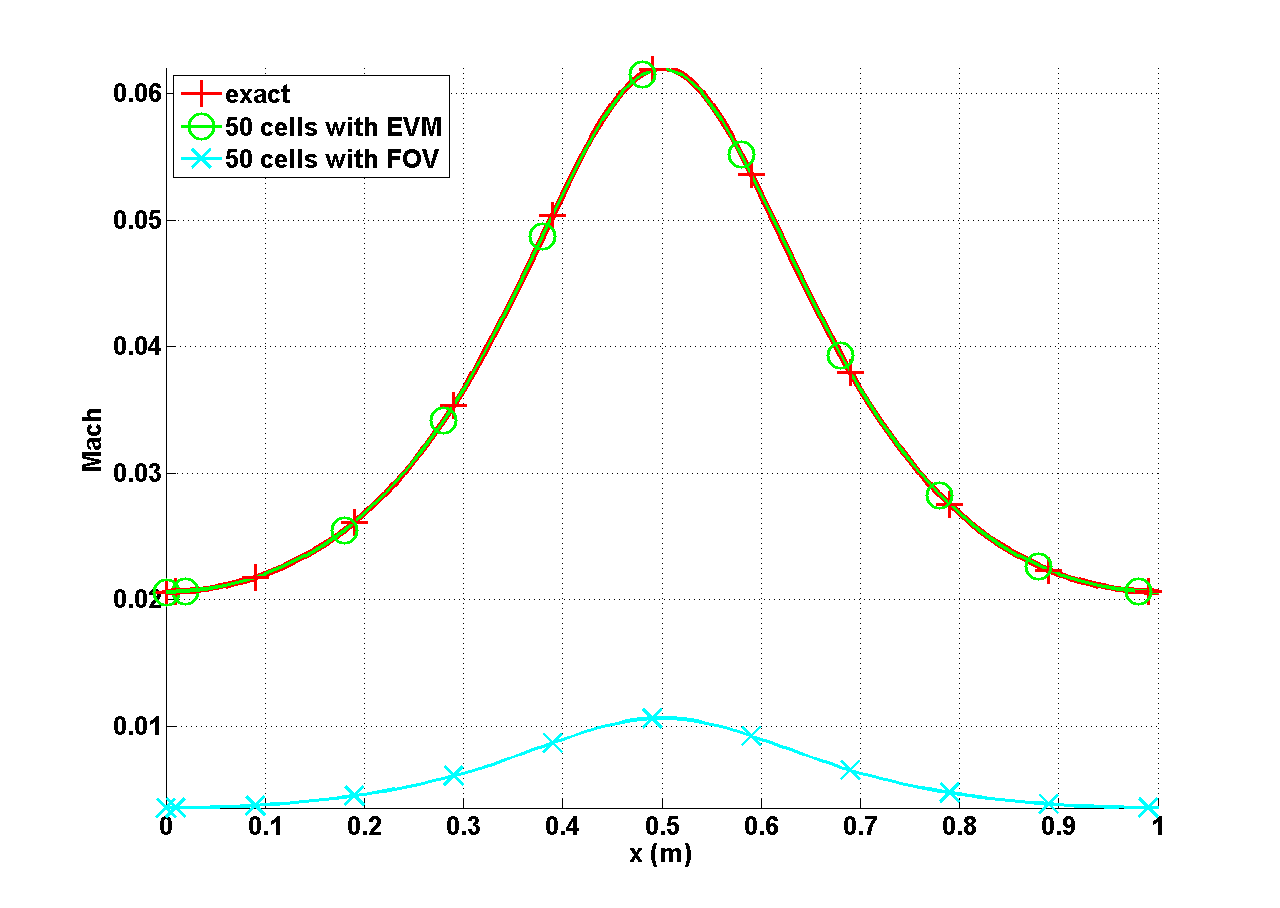
\includegraphics[width=\textwidth]{liquid_mach_numerical_and_exact_50.png}
                \caption{Mach number}
                \label{fig:1d_nozzle_liq_vel}
        \end{subfigure}%
        %add desired spacing between images, e. g. ~, \quad, \qquad etc. 
          %(or a blank line to force the subfigure onto a new line)
        \begin{subfigure}[b]{0.495\textwidth}
                \centering
                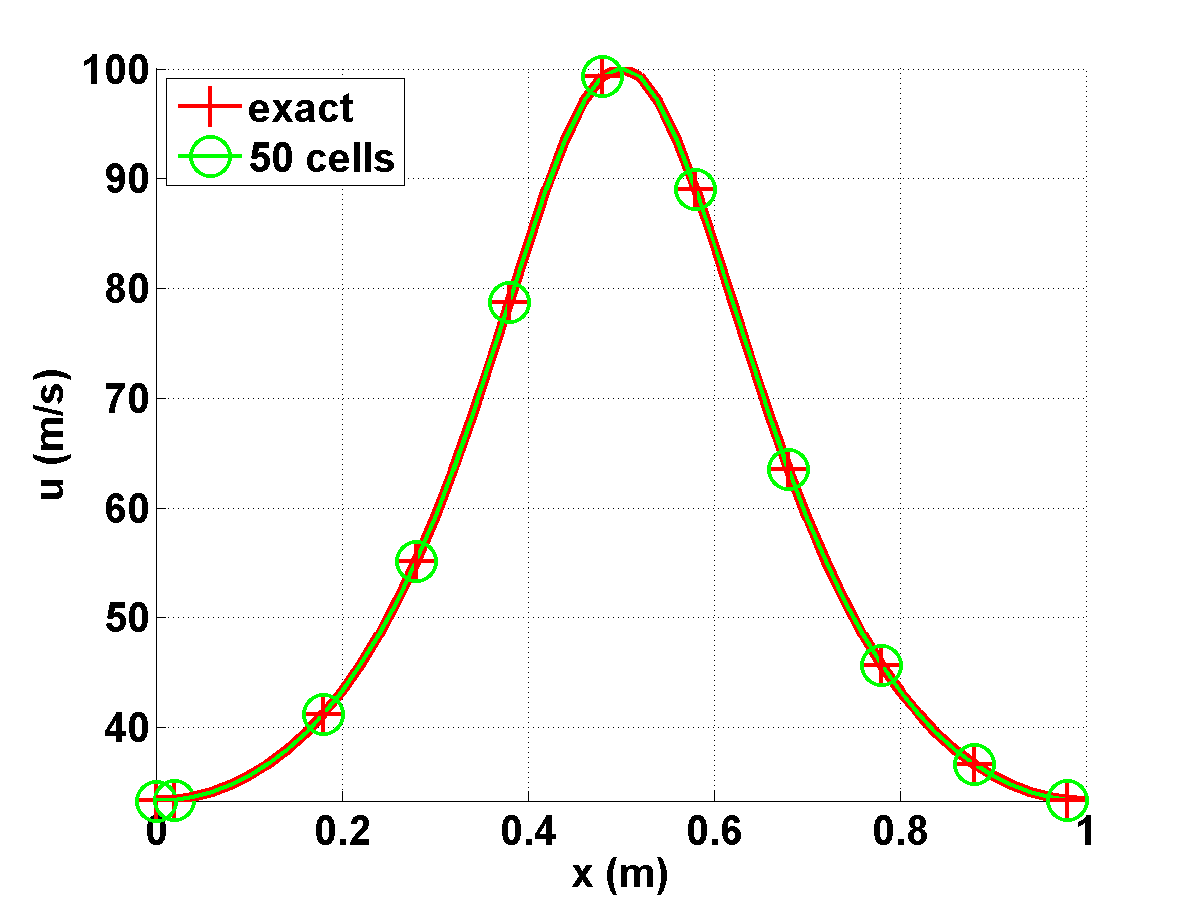
\includegraphics[width=\textwidth]{liquid_density_numerical_and_exact_50.png}
                \caption{Density}
                \label{fig:1d_nozzle_liq_density}
        \end{subfigure}

        \begin{subfigure}[b]{0.495\textwidth}
                \centering
                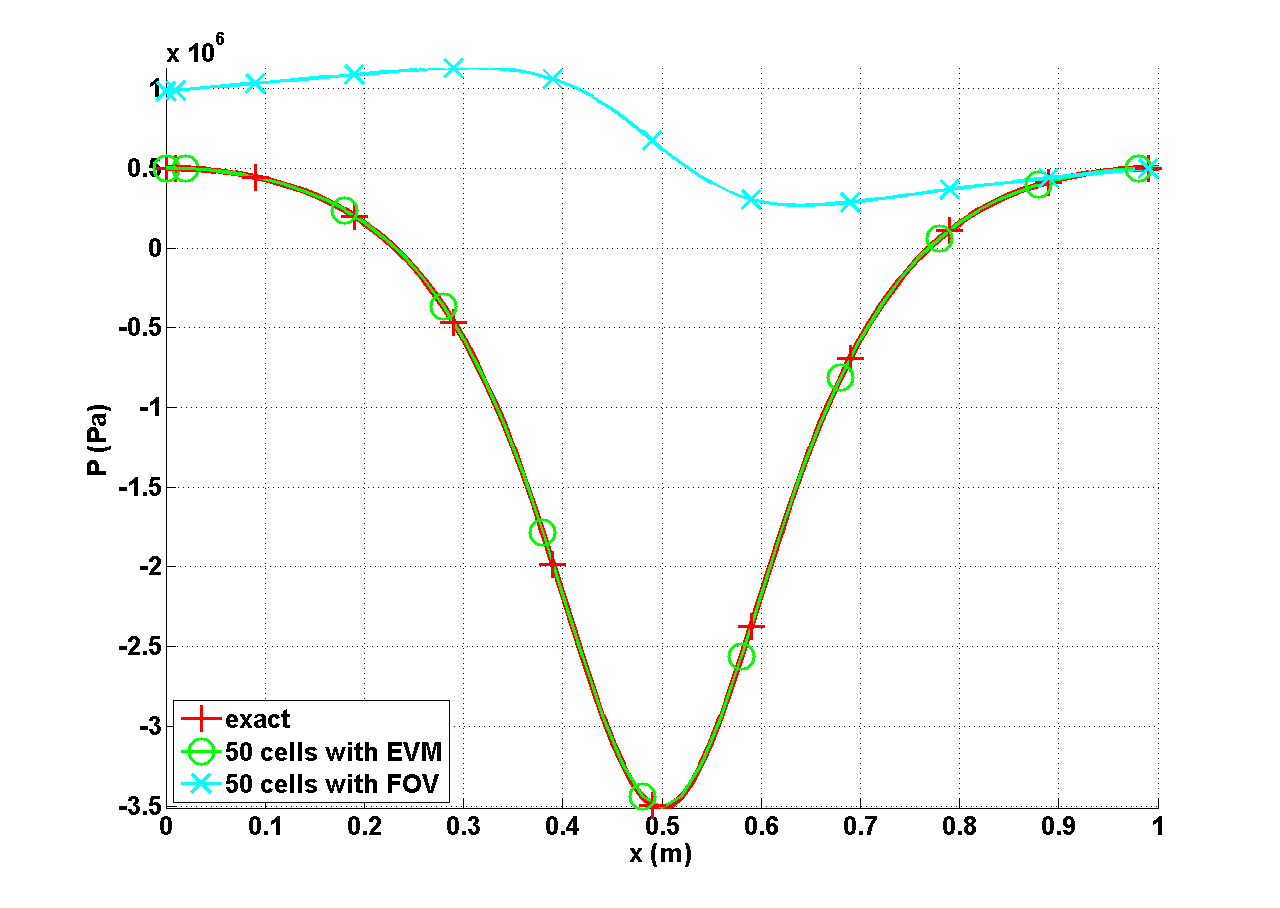
\includegraphics[width=\textwidth]{liquid_pressure_numerical_and_exact_50.png}
                \caption{Pressure}
                \label{fig:1d_nozzle_liq_press}
        \end{subfigure}

        \begin{subfigure}[b]{0.495\textwidth}
                \centering
                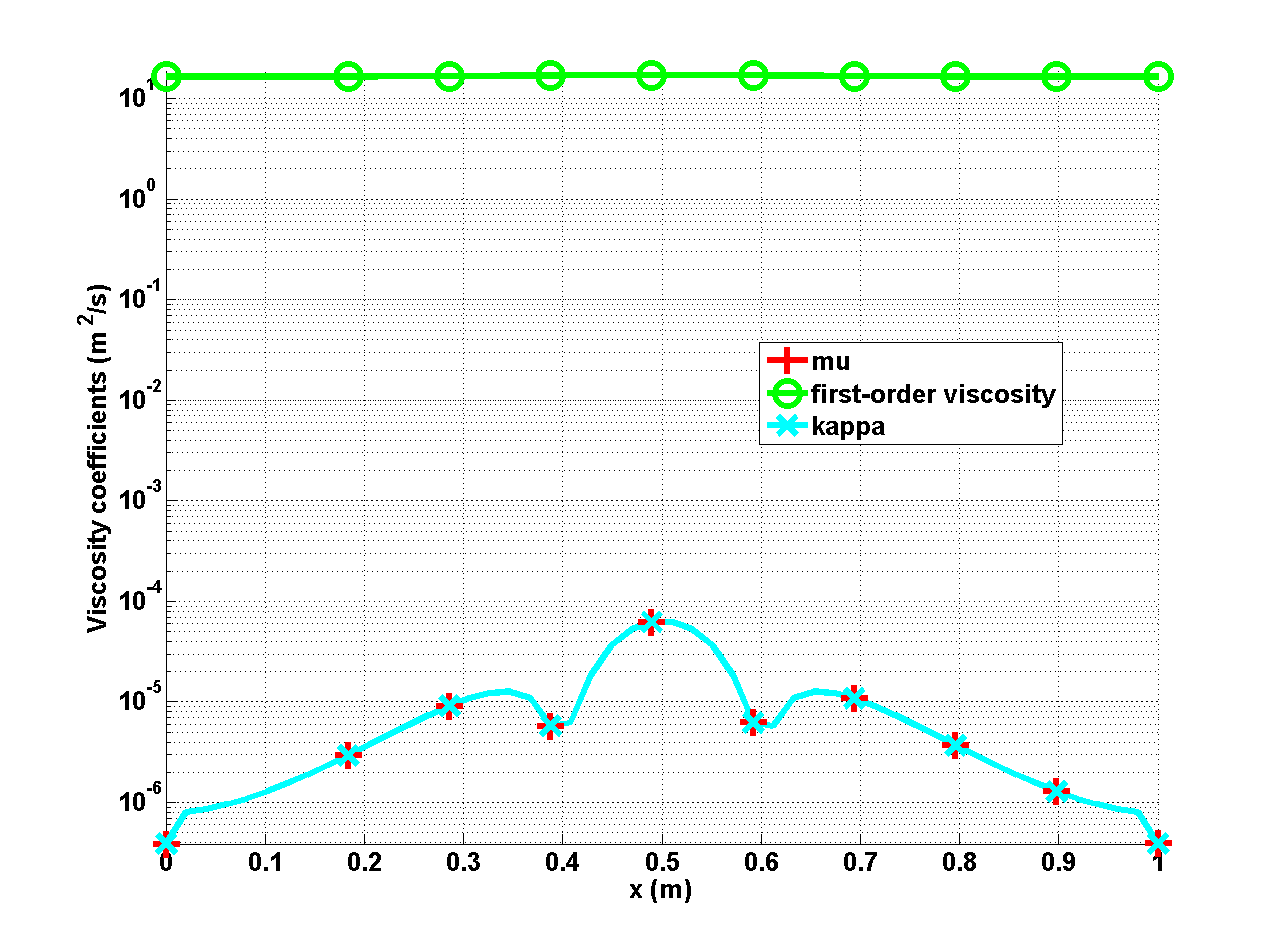
\includegraphics[width=\textwidth]{liquid_viscosity_numerical50.png}
                \caption{Viscosity coefficients}
                \label{fig:1d_nozzle_liq_visc}
        \end{subfigure}
        \caption{Steady-state solution for a liquid flow through a 1-D convergent-divergent nozzle.}\label{fig:1d_liq_nozzle}
\end{figure}
%
In \fig{fig:1d_liq_nozzle}, the numerical solutions obtained using the first-order viscosity (FOV) and the entropy viscosity method (EVM) are plotted against the exact solution. The numerical solution obtained with the EVM and the exact solution overlap, even for fairly coarse mesh (50 cells).
On the other hand, the numerical solution obtained with the FOV does not give the correct steady-state: this is an illustration of the effect of ill-scaled dissipative terms. 
%
Note that the entropy viscosity coefficient is very small compared to the first-order one (\fig{fig:1d_nozzle_liq_visc}): (i) the numerical solution is smooth as shown in \fig{fig:1d_liq_nozzle} and (ii) the flow is in a low Mach regime and thus isentropic . A convergence study was performed using the exact solution as a reference: the L$_1$ and L$_2$ norms of the error and the corresponding convergence rates are computed at steady-state on various uniform mesh from 4 to 256 cells. Spatial convergence results using linear finite elements are reported in \tbl{tbl:l1_norm_liq} and \tbl{tbl:l2_norm_liq} for the primitive variables: density, velocity and pressure.
%
\begin{table}[H]
\begin{center}
 \caption{\label{tbl:l1_norm_liq} L$_1$ norm of the error for the liquid phase in a 1-D convergent-divergent nozzle at steady-state.}
 \begin{tabular}{|c|c|c|c|c|c|c|c|c|}
 \hline
cells & density         & rate   & pressure        & rate    & velocity         & rate     \\ \hline
4    & 2.8037 $10^{-1}$ & $-$    & 8.4705 $10^{5}$ & $-$     & 7.2737           & $-$      \\ \hline
8    & 1.3343 $10^{-1}$ & 1.0713 & 4.7893 $10^{5}$ & 0.24227 & 6.1493           & 0.074683 \\ \hline
16   & 2.9373 $10^{-2}$ & 2.1835 & 1.0613 $10^{5}$ & 2.3247  & 1.2275           & 2.4501   \\ \hline
32   & 5.1120 $10^{-3}$ & 2.5225 & 1.8446 $10^{4}$ & 2.6959  & 1.8943 $10^{-1}$ & 3.0966   \\ \hline
64   & 1.0558 $10^{-3}$ & 2.2755 & 3.7938 $10^{3}$ & 2.3207  & 3.7919 $10^{-2}$ & 2.3323   \\ \hline
128  & 2.3712 $10^{-4}$ & 2.1547 & 8.4471 $10^{2}$ & 2.0624  & 8.5517 $10^{-3}$ & 2.0473   \\ \hline
256  & 5.6058 $10^{-5}$ & 2.0806 & 1.9839 $10^{2}$ & 2.0478  & 2.0475 $10^{-3}$ & 1.9833   \\ \hline
512  & 1.3278 $10^{-5}$ & 2.0778 & 4.6622 $10^{1}$ & 2.0478  & 4.9516 $10^{-4}$ & 1.9669   \\ \hline
\end{tabular}
\end{center}
\end{table}
%
\tcb{I did 
\begin{equation}
c = \frac{P_1}{P_2}
\end{equation}
Valentin did the same thing in his paper.
}
\tcr{In \tbl{tbl:l1_norm_liq}, I cannot get your rate values. For example, set
\begin{eqnarray*}
P_1 &=& 8.4471 \times 10^{2} \\
P_2 &=& 1.9839 \times 10^{2} \\
P_3 &=& 4.6622 \times 10^{1} \\
\end{eqnarray*}
then the convergence order can be estimated as
\[
c = \frac{P_2-P_1}{P_3-P_2} = \frac{((1/2)^q-1)h^q}{((1/2)^q-1)(h/2)^q}=2^q
\]
thus
\[
q = \frac{\log{c}}{\log{2}}
\]
Here, $c= 4.2586052395762$ and $q=2.0903810024167$. Since the last two pressure rate values in your table are identical, 2.0478, maybe it is a copy/paste mistake. So, let's try again with other pressure values:
\begin{eqnarray*}
P_1 &=& 3.7938 \times 10^{3} \\
P_2 &=& 8.4471 \times 10^{2} \\
P_3 &=& 1.9839 \times 10^{2} \\
\end{eqnarray*}
Now, $c= 4.56289454140364$ and $q=2.18994931029196$. What is happening?
}
%
\begin{table}[H]
\begin{center}
 \caption{\label{tbl:l2_norm_liq} L$_2$ norm of the error for the liquid phase in a 1-D convergent-divergent nozzle at steady-state.}
 \begin{tabular}{|c|c|c|c|c|c|c|c|c|}
 \hline
cells& density            & rate & pressure          & rate & velocity           & rate \\ \hline
4    & 3.106397 $10^{-1}$ & $-$  & 5.254445 $10^{5}$ & $-$  & 3.288543           & $-$  \\ \hline
8    & 7.491623 $10^{-2}$ & 2.07 & 1.636966 $10^{5}$ & 1.60 & 1.823880           & 0.90 \\ \hline
16   & 2.079858 $10^{-2}$ & 1.80 & 4.627338 $10^{4}$ & 1.75 & 4.990605 $10^{-1}$ & 1.83 \\ \hline
32   & 5.329627 $10^{-3}$ & 1.90 & 1.180287 $10^{4}$ & 1.92 & 1.261018 $10^{-1}$ & 1.93 \\ \hline
64   & 1.341583 $10^{-3}$ & 1.94 & 2.967104 $10^{3}$ & 1.98 & 3.160914 $10^{-2}$ & 1.99 \\ \hline
128  & 3.359766 $10^{-4}$ & 1.99 & 7.428087 $10^{2}$ & 1.99 & 7.907499 $10^{-3}$ & 1.99 \\ \hline
256  & 8.403859 $10^{-5}$ & 1.99 & 1.857861 $10^{2}$ & 1.99 & 1.977292 $10^{-3}$ & 1.99 \\ \hline
512  & 2.10075  $10^{-5}$ & 1.99 & 2.7048   $10^{1}$ & 1.99 & 4.9516   $10^{-4}$ & 1.99 \\ \hline
\end{tabular}
\end{center}
\end{table}
\tcr{check the rates in this table as well\\}
It is observed that the convergence rate for the L$_1$ and L$_2$ norm of the error is 2: the entropy viscosity method preserves the high-order accuracy when the numerical solution is smooth, and the new definition of the entropy viscosity coefficient behaves appropriately in the low-Mach limit.

%---------------------------------------------------------------------------------------------------
\subsection{Steam in a 1-D divergent-convergent nozzle} \label{sec:steam_nozzle}
%---------------------------------------------------------------------------------------------------

We use the same nozzle geometry, initial conditions and boundary conditions as in the previously example but replace liquid water with steam and use the steam parameters of the stiffened gas equation of state, \tbl{tbl:stff_gas_eos}. In this run, compressible effects will become dominant. 
The pressure difference between the inlet and outlet is large enough to accelerate the steam through the nozzle, leading to a formation of shock in the divergent portion of the nozzle. The behavior is different from what was observed for the liquid water phase in \sct{sec:liquid_nozzle} because of the liquid to gas density ratio is about $1,000$. An exact solution at steady-state is available for the gas phase \cite{nozzle_exact}. The aim of this section is to show that when using the new definitions of the viscosity coefficients (\eqt{eq:final_def_visc_coeff}), the shock can be correctly resolved without spurious oscillations. The steady-state numerical solution, obtained using a uniform mesh with $1600$ cells, is shown in \fig{fig:1d_vap_nozzle}. The $CFL$ was set to $80$ (a high $CFL$ value can be used since the shock is stationary).

\begin{figure}[H]
        \centering
        \begin{subfigure}[b]{0.495\textwidth}
                \centering
                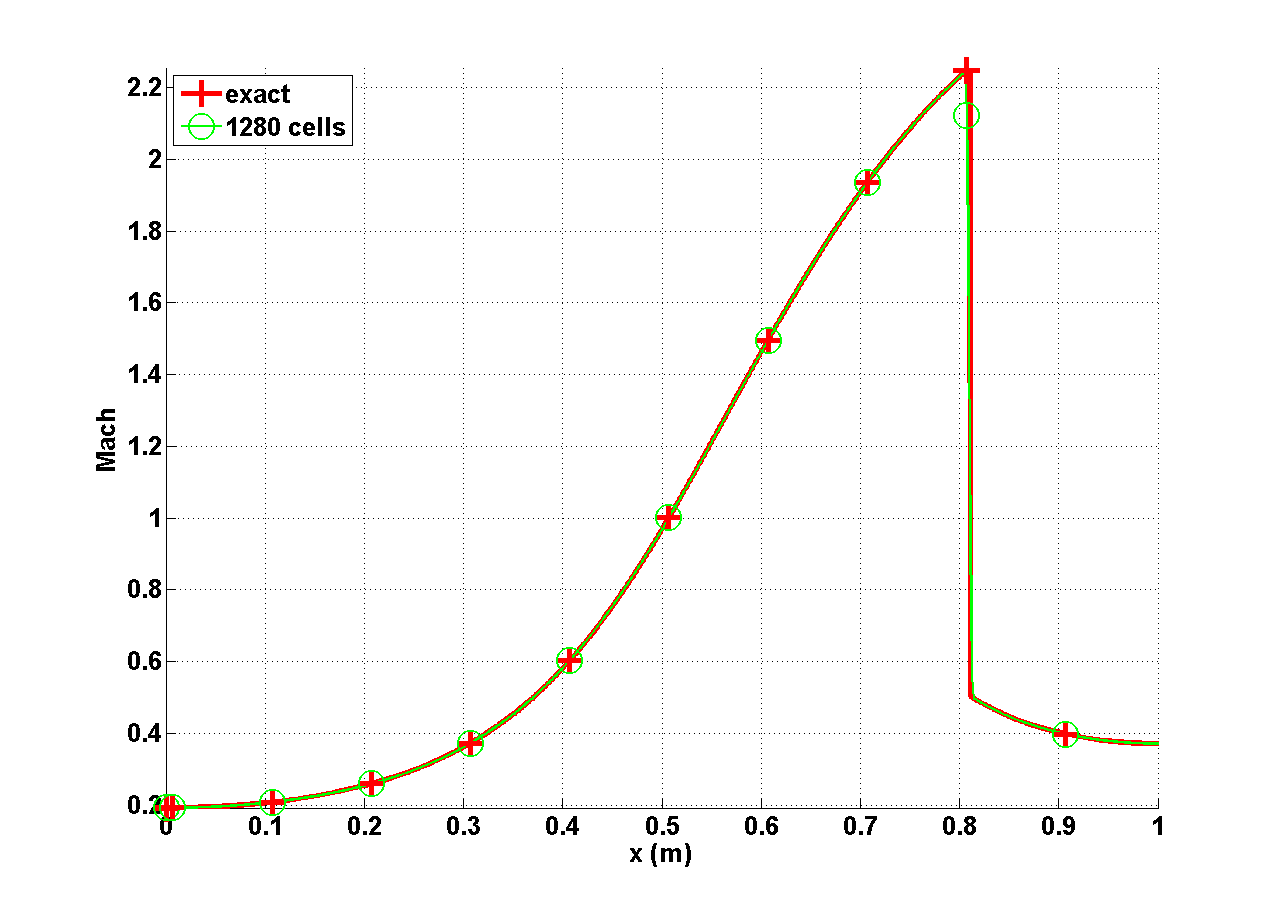
\includegraphics[width=\textwidth]{vapor_mach_numerical_and_exact_1280.png}
                \caption{Mach number}
                \label{fig:1d_nozzle_vap_vel}
        \end{subfigure}%

        \begin{subfigure}[b]{0.495\textwidth}
                \centering
                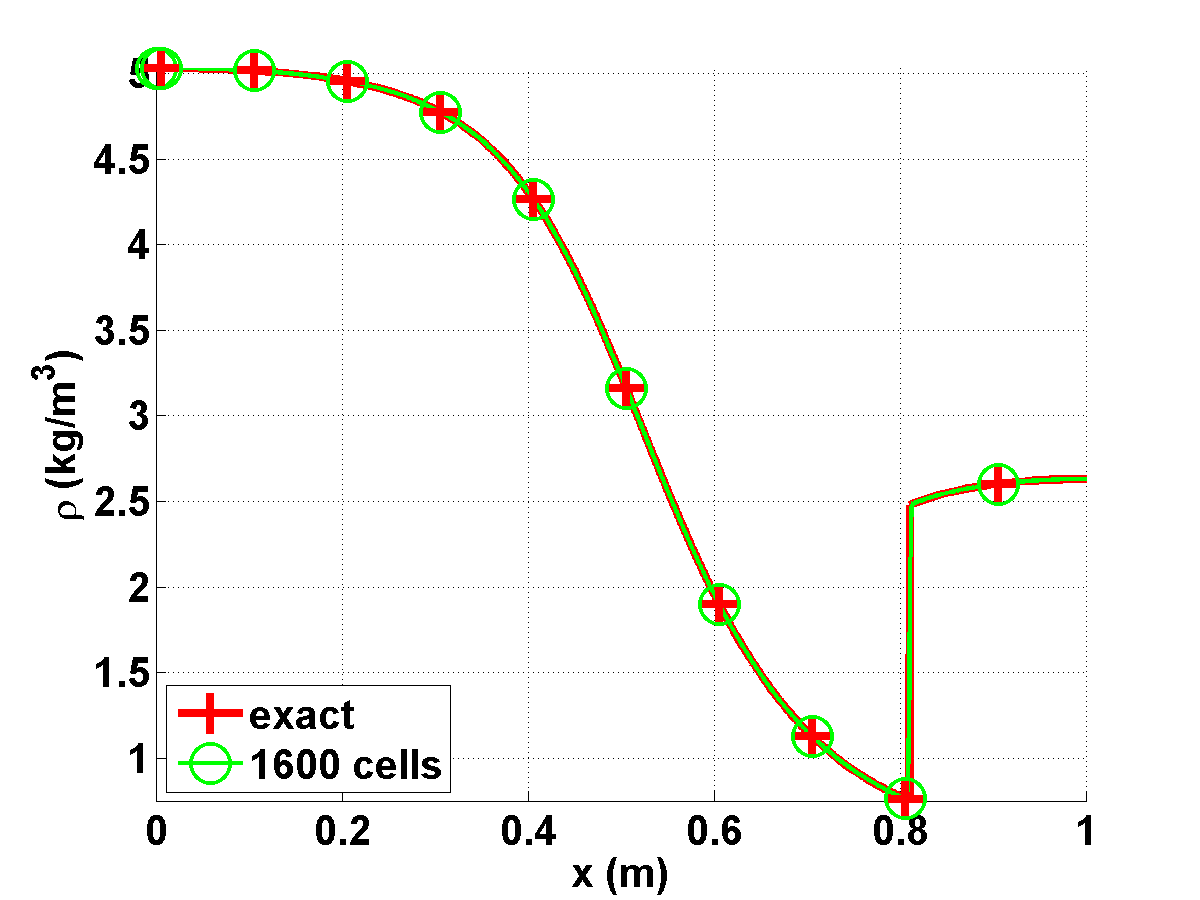
\includegraphics[width=\textwidth]{vapor_density_numerical_and_exact_1600.png}
                \caption{Density}
                \label{fig:1d_nozzle_vap_density}
        \end{subfigure}

        \begin{subfigure}[b]{0.495\textwidth}
                \centering
                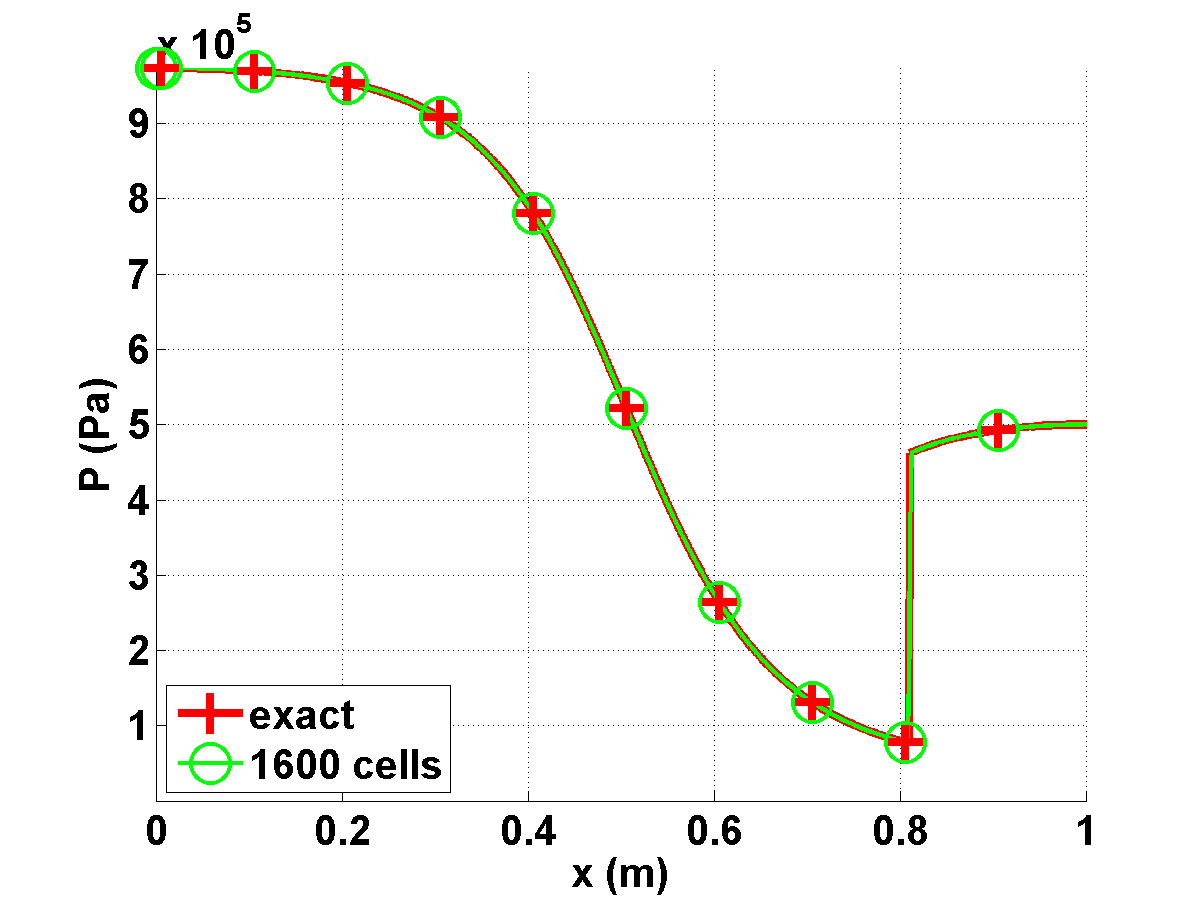
\includegraphics[width=\textwidth]{vapor_pressure_numerical_and_exact_1600.png}
                \caption{Pressure}
                \label{fig:1d_nozzle_vap_press}
        \end{subfigure}

        \begin{subfigure}[b]{0.495\textwidth}
                \centering
                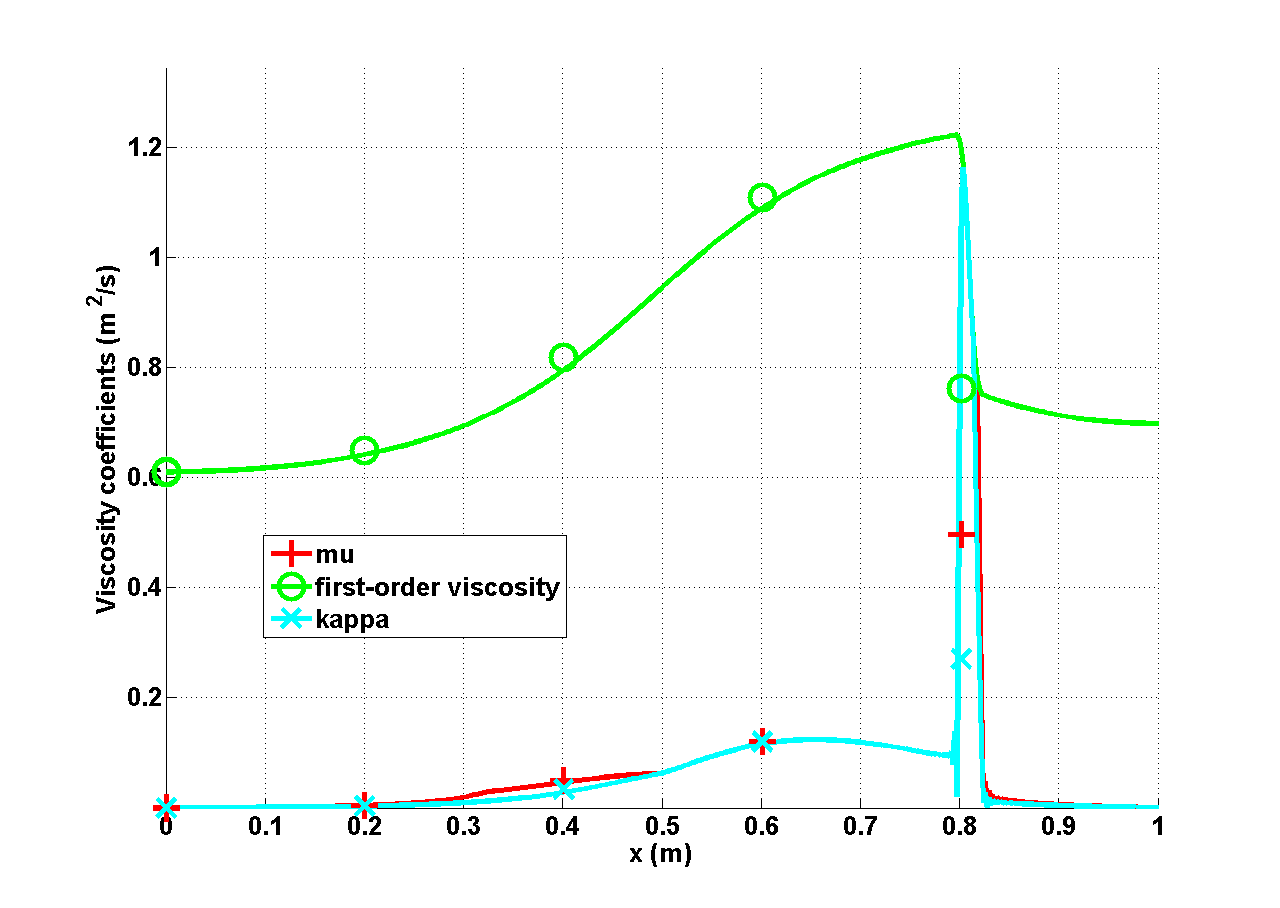
\includegraphics[width=\textwidth]{vapor_viscosity_numerical1600.png}
                \caption{Viscosity coefficients}
                \label{fig:1d_nozzle_vap_visc}
        \end{subfigure}
        \caption{Steady-state solution for vapor phase in the 1-D convergent-divergent nozzle.}
				\label{fig:1d_vap_nozzle}
\end{figure}
%
The steady-state solution of the density, Mach number and pressure are given in \fig{fig:1d_nozzle}. The steady-solution exhibits a shock around $x=0.8m$ and matches the exact solution. In \fig{fig:1d_nozzle_vap_visc}, the first-order and entropy viscosity coefficients are plotted at steady-state (on a log scale): the entropy viscosity coefficient is peaked in the shock region around $x=0.8m$ as expected where it saturates to the first-order viscosity coefficient. The graph also presents another peak at $x=0.5m$  corresponding to the position of the sonic point for a 1-D convergent-divergent nozzle. This particular point is known to develop small instabilities that are detected when computing the jumps of the pressure and density gradients. Anywhere else, the entropy  viscosity coefficient is small. In order to prove convergence of the numerical solution to the exact solution, a convergence study is performed. Because of the presence of a shock, second-order accuracy is not expected and the convergence rate of a numerical solution should be $1$ and $1/2$ when measured in the L$_1$ and L$_2$ norms, respectively (see Theorem 9.3 in \cite{convergence_book}). Results are reported in \tbl{tbl:l1_norm_vap} and \tbl{tbl:l2_norm_vap} for the primitive variables: density, velocity and pressure. The convergence rates for the L$_1$ and L$_2$ norms of the error are in good agreement with the theoretical values.
%
\begin{table}[!htbp]
\begin{center}
 \caption{\label{tbl:l1_norm_vap} L$_1$ norm of the error for the vapor phase in a 1-D convergent-divergent nozzle at steady-state.}
 \begin{tabular}{|c|c|c|c|c|c|c|c|c|}
 \hline
cells & density              & rate      & pressure          & rate      & velocity & rate      \\ \hline
$5$  & $0.72562$   $10^{-1}$ & $-$       & $1.5657$ $10^{5}$ & $-$       & $173.69$ & $-$       \\ \hline
$10$ & $0.4165$    $10^{-1}$ & $0.80088$ & $9.6741$ $10^{4}$ & $0.63425$ & $120.69$ & $0.52519$ \\ \hline
$20$ & $0.20675$   $10^{-1}$ & $1.0104$  & $4.9193$ $10^{4}$ & $0.96971$ & $72.149$ & $0.74228$ \\ \hline
$40$ & $0.093703$  $10^{-1}$ & $1.1417$  & $2.0103$ $10^{4}$ & $0.72728$ & $34.716$ & $1.0554$  \\ \hline
$80$ & $0.047328$  $10^{-1}$ & $0.9854$  & $1.0208$ $10^{4}$ & $0.9777$  & $16.082$ & $1.1101$  \\ \hline
$160$& $0.023965$  $10^{-2}$ & $0.9817$  & $5.1969$ $10^{3}$ & $0.9739$  & $7.9573$ & $1.0150$  \\ \hline
$320$& $0.020768$  $10^{-2}$ & $0.9886$  & $2.5116$ $10^{3}$ & $1.0490$  & $3.7812$ & $1.0734$  \\ \hline
$640$& $0.0059715$ $10^{-2}$ & $1.0160$  & $1.2754$ $10^{3}$ & $0.9776$  & $1.8353$ & $1.0428$  \\ \hline
\end{tabular}
\end{center}
\nonumber
\end{table}
\begin{table}[H]
\begin{center}
 \caption{\label{tbl:l2_norm_vap} L$_2$ norm of the error for the vapor phase in a 1-D convergent-divergent nozzle at steady-state.}
 \begin{tabular}{|c|c|c|c|c|c|c|c|c|}
 \hline
cells & density             & rate      & pressure          & rate      & velocity & rate       \\ \hline
$5$   & $9.7144$ $10^{-1}$  & $-$       & $2.0215$ $10^{5}$ & $-$       & $236.94$ & $-$        \\ \hline
$10$  & $5.9718$ $10^{-1}$  & $0.70195$ & $1.3024$ $10^{5}$ & $0.63425$ & $166.56$ & $0.50854$  \\ \hline
$20$  & $2.9503$ $10^{-1}$  & $1.0173$  & $6.6503$ $10^{4}$ & $0.96971$ & $103.36$ & $0.68831$  \\ \hline
$40$  & $1.8193$ $10^{-1}$  & $0.69747$ & $4.0171$ $10^{4}$ & $0.72728$ & $66.374$ & $0.6390$   \\ \hline
$80$  & $1.3366$ $10^{-1}$  & $0.44485$ & $2.3163$ $10^{4}$ & $0.43576$ & $42.981$ & $0.62692$  \\ \hline
$160$ & $9.6638$ $10^{-2}$  & $0.46790$ & $1.7263$ $10^{4}$ & $0.42413$ & $31.717$ & $0.43844$  \\ \hline
$320$ & $7.0896$ $10^{-2}$  & $0.44688$ & $1.2763$ $10^{4}$ & $0.43571$ & $23.138$ & $0.45499$  \\ \hline
$640$ & $5.2191$ $10^{-2}$  & $0.44190$ & $9.4217$ $10^{3}$ & $0.43790$ & $16.910$ & $0.45238$  \\ \hline
\end{tabular}
\end{center}
\nonumber
\end{table}

%---------------------------------------------------------------------------------------------------
\subsection{Leblanc shock tube} \label{sec:Leblanc}
%---------------------------------------------------------------------------------------------------

The 1-D Leblanc shock tube is a Riemann problem designed to test the robustness and the accuracy of stabilization methods. The initial conditions are given in \tbl{tbl:ic_1d_tests}. The ideal gas equation of state (with $\gamma=5/3$) is used to compute the pressure.
This test is computationally challenging because of the large pressure ratio at the shock interface.
The computational domain consists of a 1-D straight pipe of length $L=9m$ with the initial interface located at $x=2m$. At $t=0.s$, the interface is removed. The numerical solution is run until $t=4 s$ and the density, momentum and total energy profiles are given in \fig{fig:1d_leblanc}, along with the exact solution. The viscosity coefficients are also plotted in \fig{fig:1d_leblanc_visc}. These plots were  run with three different uniform mesh of $800$, $3200$ and $6000$ cells and a constant $CFL = 1$.
\begin{figure}[H]
        \centering
        \begin{subfigure}[b]{0.495\textwidth}
                \centering
                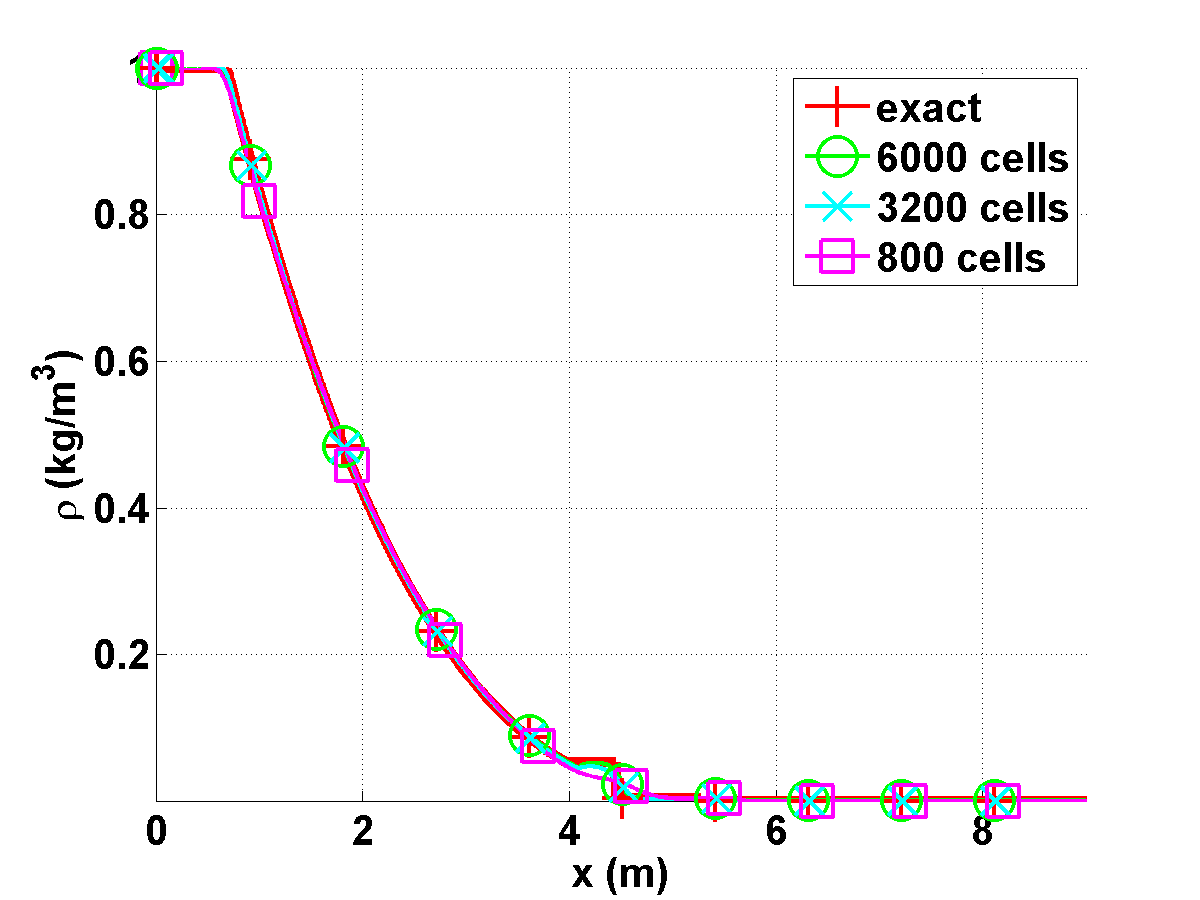
\includegraphics[width=\textwidth]{Leblanc_exact_and_numerical_stt_density_6000.png}
                \caption{Density}
                \label{fig:1d_leblanc_vel}
        \end{subfigure}%
        %add desired spacing between images, e. g. ~, \quad, \qquad etc. 
          %(or a blank line to force the subfigure onto a new line)
        \begin{subfigure}[b]{0.495\textwidth}
                \centering
                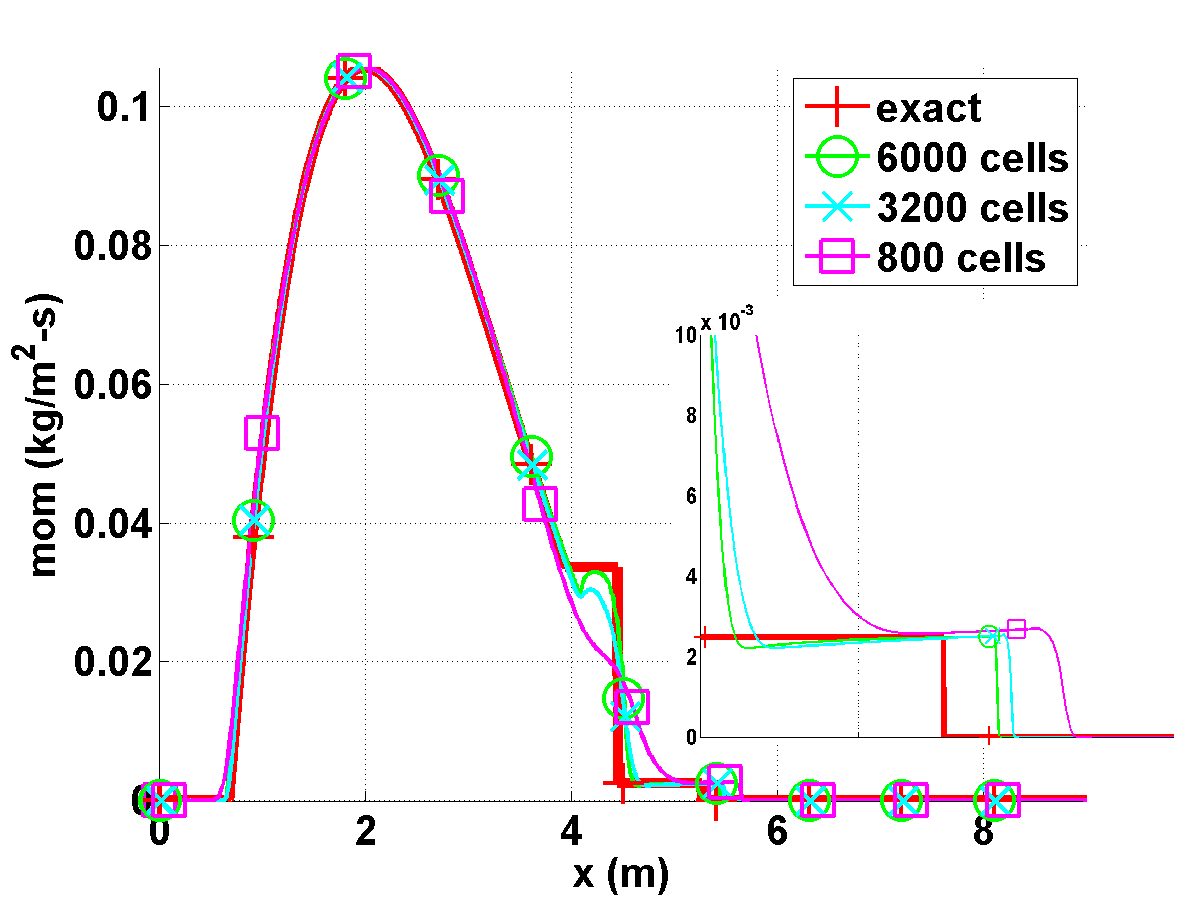
\includegraphics[width=\textwidth]{Leblanc_exact_and_numerical_stt_momentum_6000.png}
                \caption{Momentum}
                \label{fig:1d_leblanc_density}
        \end{subfigure}
         %add desired spacing between images, e. g. ~, \quad, \qquad etc. 
          %(or a blank line to force the subfigure onto a new line)
        \begin{subfigure}[b]{0.495\textwidth}
                \centering
                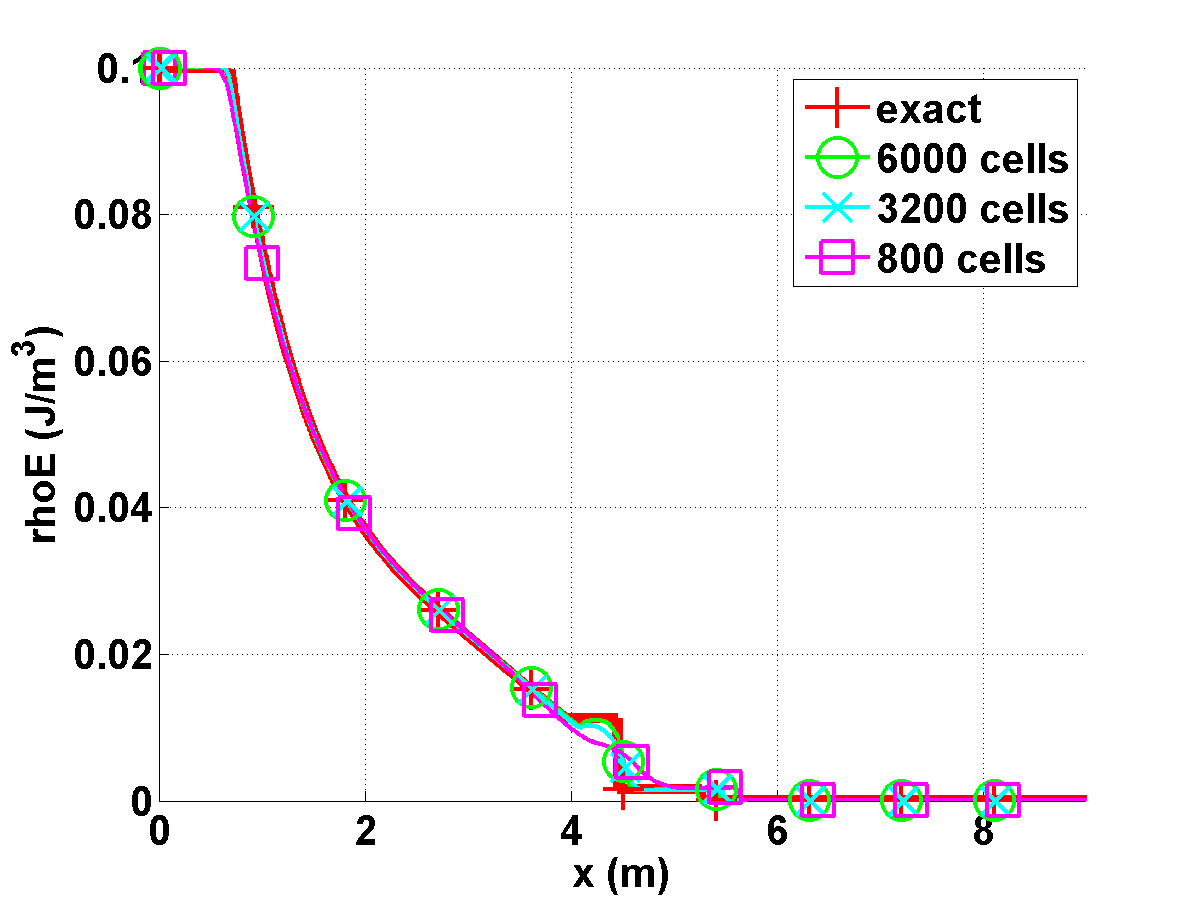
\includegraphics[width=\textwidth]{Leblanc_exact_and_numerical_stt_total_energy_6000.png}
                \caption{Total energy}
                \label{fig:1d_leblanc_press}
        \end{subfigure}
          %add desired spacing between images, e. g. ~, \quad, \qquad etc. 
          %(or a blank line to force the subfigure onto a new line)
        \begin{subfigure}[b]{0.495\textwidth}
                \centering
                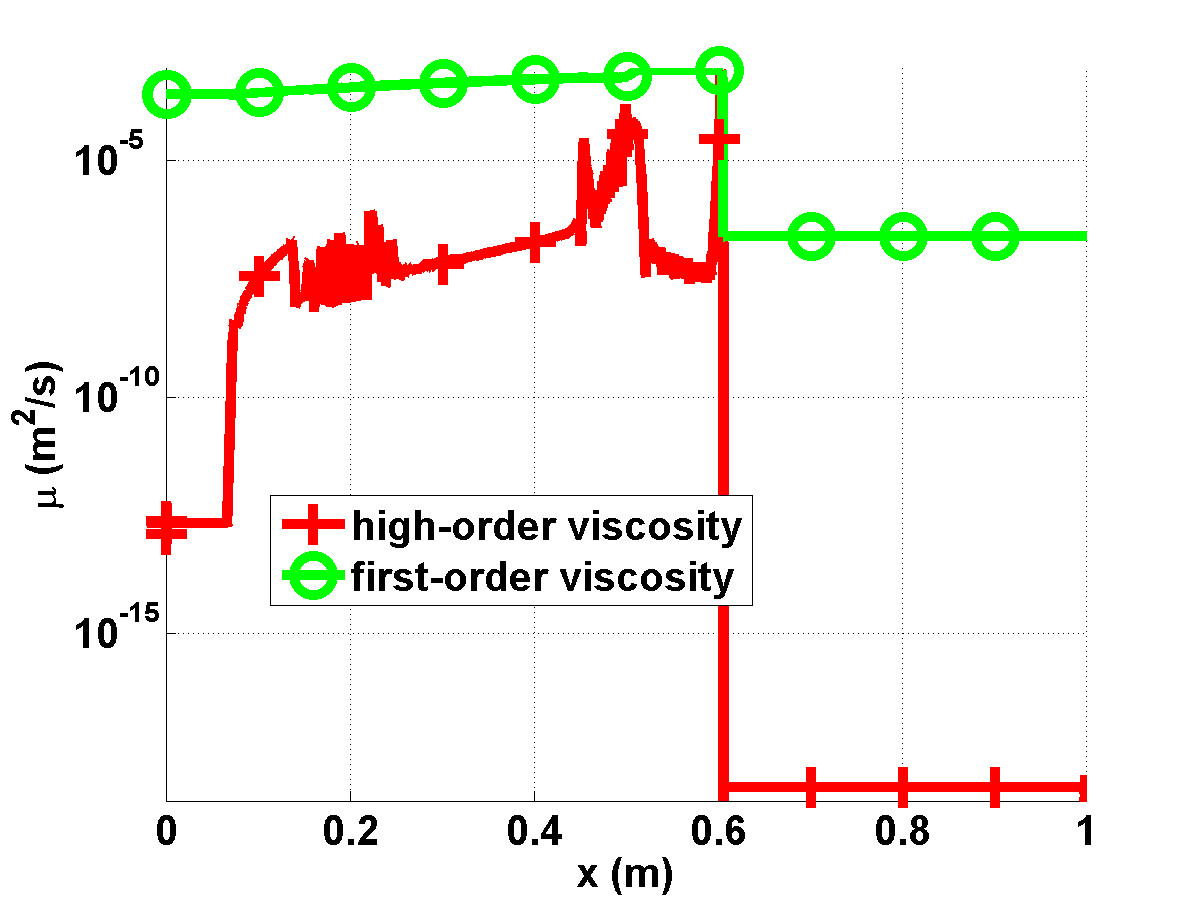
\includegraphics[width=\textwidth]{Leblanc_viscosity_numerical_6000.png}
                \caption{Viscosity coefficients}
                \label{fig:1d_leblanc_visc}
        \end{subfigure}
        \caption{Exact and Numerical solutions for the 1-D Leblanc shock tube at $t=4 s$.}\label{fig:1d_leblanc}
\end{figure}
%
The density, momentum and total energy profiles are provided in \fig{fig:1d_leblanc}. In \fig{fig:1d_leblanc_density}, the shock region is zoomed in for better resolution: the shock is well resolved and do not present any oscillations. We also observed that the shock position computed numerically converges to the exact position under mesh refinement. The contact wave at $x=4.5m$ can be seen in \fig{fig:1d_leblanc_density}. The entropy viscosity coefficient profile is shown in \fig{fig:1d_leblanc_visc} and behaves as expected: it saturates to the first-order viscosity in the shock region, thus preventing oscillations from forming. At the location of the contact wave, a smaller peak is observed that is due to the presence of the jumps in the definition of the entropy viscosity coefficient (\eqt{eq:final_def_visc_coeff}).  The Mach number, not plotted, is of the order of $1.3$ right before the shock and reaches a maximum value close to $5$ in the contact region.\tcr{you said it was also subsonic. where?} \tcb{No it is not.}\\
Once again, a convergence study is performed in order to prove convergence of the numerical solution to the exact solution. As in the previous example (the vapor phase in the 1-D nozzle, \sct{sec:steam_nozzle}), the expected convergence rates in the L$_1$ and L$_2$ norms are $1$ and $1/2$, respectively. The exact solution was obtained by running a 1-D Riemann solver and used as the reference solution to compute the L$_1$ and L$_2$-norms that are reported in \tbl{tbl:l1_norm_leblanc} and \tbl{tbl:l2_norm_leblanc} for the conservative variables: density, momentum and total energy. The convergence rates are approaching the theoretical values.

\begin{table}[!htbp]
\begin{center}
 \caption{\label{tbl:l1_norm_leblanc} L$_1$ norm of the error for the 1-D Leblanc test at $t=4s$.}
 \begin{tabular}{|c|c|c|c|c|c|c|c|c|}
 \hline
  cells & density               & rate         & momentum              & rate          & total energy          & rate         \\  \hline
$100$   & $1.0354722$ $10^{-2}$ & $-$          & $3.5471714$ $10^{-3}$ & $-$           & $1.4033046$ $10^{-3}$ & $-$          \\  \hline
$200$   & $7.2680512$ $10^{-3}$ & $0.51064841$ & $2.5933119$ $10^{-3}$ & $0.45187331$  & $9.8611746$ $10^{-4}$ & $0.5089968$  \\  \hline
$400$   & $5.0825628$ $10^{-3}$ & $0.51601245$ & $2.0668092$ $10^{-3}$ & $0.32739054$  & $7.7844421$ $10^{-4}$ & $0.34116585$ \\  \hline
$800$   & $3.4025056$ $10^{-3}$ & $0.57895861$ & $1.4793838$ $10^{-3}$ & $0.48240884$  & $5.5702549$ $10^{-4}$ & $0.48285029$ \\  \hline
$1600$  & $2.1649953$ $10^{-3}$ & $0.65223363$ & $9.7152832$ $10^{-4}$ & $0.6066684$   & $3.5720171$ $10^{-4}$ & $0.64100438$ \\  \hline
$3200$  & $1.2465433$ $10^{-3}$ & $0.79643094$ & $5.5937409$ $10^{-4}$ & $0.79644263$  & $2.0491799$ $10^{-4}$ & $0.80169235$ \\  \hline
$6400$  & $6.4476928$ $10^{-4}$ & $0.95107804$ & $3.0244198$ $10^{-4}$ & $0.88715502$  & $1.0914891$ $10^{-4}$ & $0.90874889$ \\  \hline
$12800$ & $3.3950948$ $10^{-4}$ & $0.92533116$ & $1.5958118$ $10^{-4}$ & $0.9223679$   & $5.7909794$ $10^{-5}$ & $0.91441847$ \\  \hline
 \end{tabular}
\end{center}
\end{table}
%
\begin{table}[!htbp]
\begin{center}
 \caption{\label{tbl:l2_norm_leblanc} L$_2$ norm of the error for the 1-D Leblanc test at $t=4s$.}
 \begin{tabular}{|c|c|c|c|c|c|c|}
 \hline
   cells & density & rate & momentum & rate & total energy & rate \\ \hline
$100$ &   $5.7187851$ $10^{-3}$ & $-$ & $1.7767236$ $10^{-3}$ & $-$ & $7.6112265$  $10^{-4}$& $-$\\   \hline
$200$  &  $3.8995238$ $10^{-3}$ & $0.55241073$ & $1.4913161$ $10^{-3}$ & $0.25263314$ &  $5.5497308$ $10^{-4}$& $0.45571115$\\ \hline
$400$ & $2.8103526$ $10^{-3}$   & $0.4725468$ & $1.3305301$ $10^{-3}$ & $0.164585$ & $4.6063172$ $10^{-4}$ & $0.26880405$\\ \hline
$800$ & $2.1081933$ $10^{-3}$   & $0.41474398$ & $1.1398931$ $10^{-3}$ & $0.22310254$ & $3.7798953$ $10^{-4}$ & $0.28526749$\\ \hline
$1600$ & $1.5731052$ $10^{-3}$  & $0.42239201$ & $9.0394227$ $10^{-4}$ & $0.33459602$ & $2.9584646$ $10^{-4}$ & $0.35349763$\\ \hline
$3200$&$1.0610667$ $10^{-3}$    & $0.56809979$ & $6.2735595$ $10^{-4}$ & $0.52694639$ & $2.054455$ $10^{-4}$ & $0.52609289$\\ \hline
$6400$&$7.3309974$ $10^{-4}$    & $0.53343397$ & $4.4545754$ $10^{-4}$ & $0.49399631$ & $1.4670834$ $10^{-4}$ & $0.48580482$\\ \hline
 $12800$&$5.1020991$ $10^{-4}$  & $0.52291857$ & $3.1266758$ $10^{-4}$ & $0.5106583$ & $1.0299897$ $10^{-5}$ & $0.51032105$\\  \hline
\end{tabular}
\end{center}
\nonumber
\end{table}

%---------------------------------------------------------------------------------------------------
\subsection{1-D shock tube with a liquid phase} \label{sec:liquid_shock}
%---------------------------------------------------------------------------------------------------
\tcr{until now, you never gave the mu and kappa coefficients, yet they are now different due to their different normalizations.
Maybe very little for the previous cases, but we need to mention something because, in this section, you show both, and it is better
to say something than to let the reviewers wonder ... }


Here, we investigate the ability of the entropy viscosity method to resolve strong shocks in a liquid phase \tcr{I feel like we need to add a little something to justify why it is so important to study a shock in a liquid but without having to talk about 2-phase flows. can you craft something?}. This test is a preliminary work to the application of the entropy viscosity method to a two phase flow model. The stiffened gas equation of state is used to model a liquid flow with the parameters given in \tbl{tbl:stff_gas_eos}. The computational domain of length $L=1m$ is uniformly discretized using 500 cells. The step initial conditions are given in \tbl{tbl:ic_1d_tests}.
%
The simulation is run with a $CFL=1$ until the final time $t_{\text{final}} = 7 \ 10^{-5}s$. Results for pressure, density, velocity and the viscosity coefficients are given in \fig{fig:1d_strong_shock} along with the exact solution for comparison purposes. The numerical solution is in good agreement with exact solution in \fig{fig:1d_strong_shock_var}. The viscosity coefficients $\mu$ and $\kappa$ are not equal in the shock because the Mach number is of order $0.1$. The viscosity coefficient $\kappa$ saturates to the first-order viscosity in the shock region around $x = 0.65m$ and is sufficient to stabilize the numerical scheme. This example illustrates the capabilities of the entropy viscosity method to stabilize a strong shock using liquid fluid properties. 
%
\begin{figure}[H]
        \centering
        \begin{subfigure}[b]{0.495\textwidth}
                \centering
                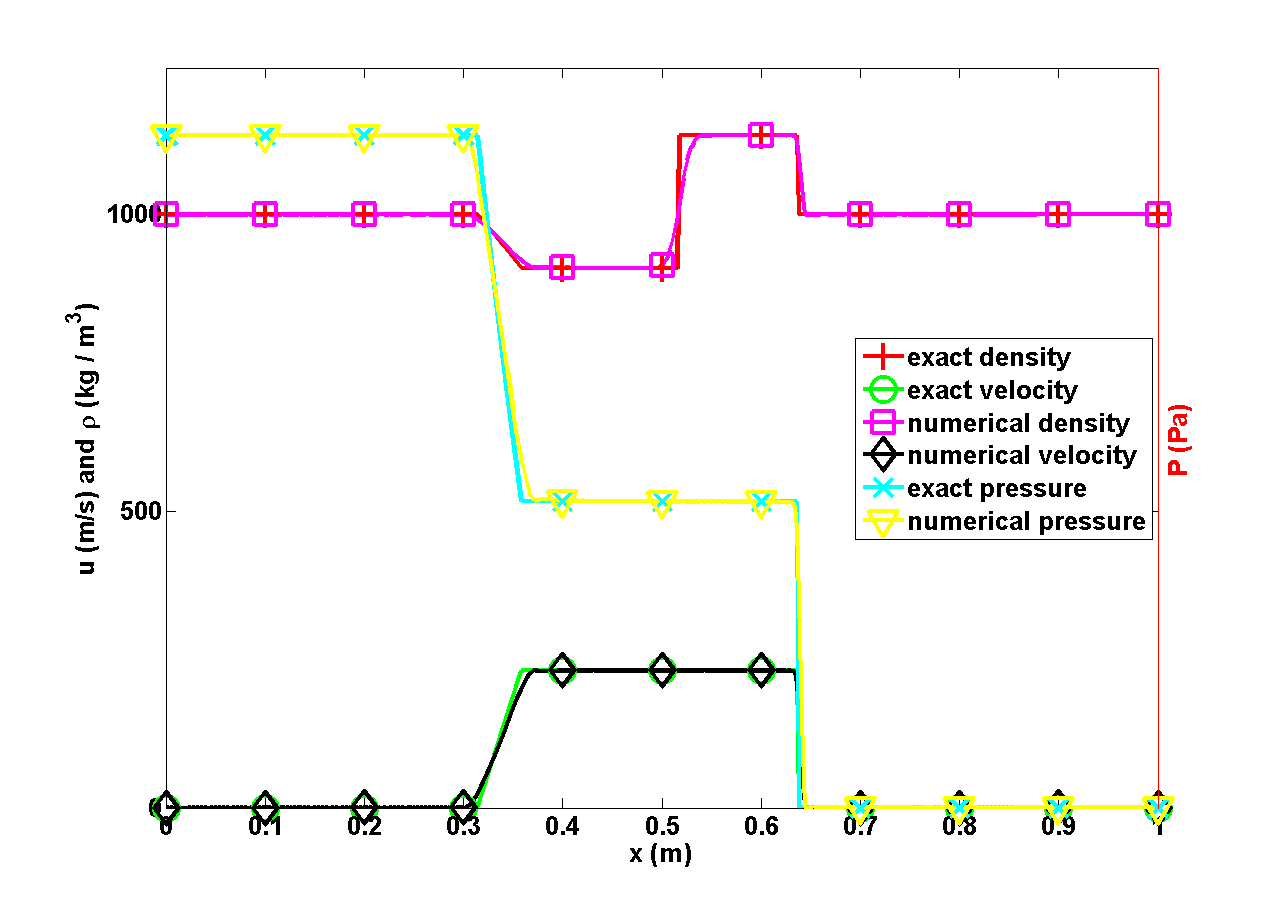
\includegraphics[width=\textwidth]{LiquidSrongShock_density_velocity_pressure_profiles.png}
                \caption{Density, velocity and pressure profiles.}
                \label{fig:1d_strong_shock_var}
        \end{subfigure}%

        \begin{subfigure}[b]{0.495\textwidth}
                \centering
                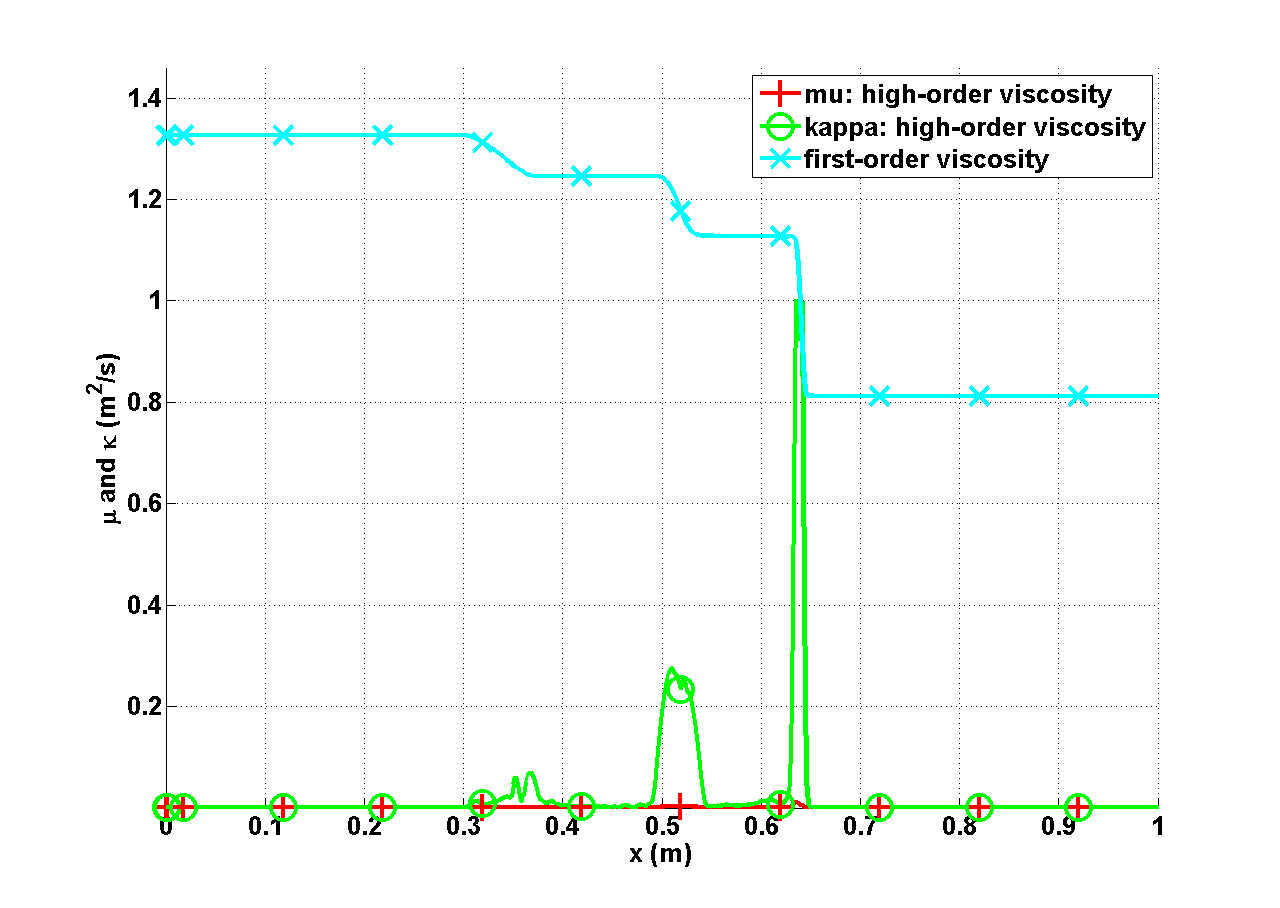
\includegraphics[width=\textwidth]{LiquidSrongShock_viscosity.png}
                \caption{Viscosity coefficients profile.}
                \label{fig:1d_strong_shock_visc}
        \end{subfigure}
        \caption{Numerical solution for the 1-D liquid shock tube at  at $t_{\text{final}} = 7 \  10^{-5}s$.}
				\label{fig:1d_strong_shock}
\end{figure}


%---------------------------------------------------------------------------------------------------
\subsection{1-D slow moving shock} \label{sec:slow_moving_shock}
%---------------------------------------------------------------------------------------------------

Slow moving shocks are known to produce post-shock noise of low frequency that are not damped by some numerical dissipation methods \cite{james}. The aim of this simulation is to test the ability of the entropy viscosity method of damping the low frequency waves.
The 1-D slow moving shock consists of a shock wave moving from left to right with the initial conditions given in \tbl{tbl:ic_1d_tests}. The ideal gas equation of state is used with a heat capacity ratio, $\gamma$, of 1.4.  In order to make the shock travel a significant distance, the final time is taken equal to $t=1.1s$. A pressure boundary condition is used at the left boundary to let the rarefaction and contact waves exit the domain.   
%
The numerical solution, obtained with 200 equally-spaced cells, is given in \fig{fig:low_moving_shock} and is compared to the exact solution obtained from a Riemann solver. We use a $CFL$ of $1$. With this $CFL$ value, it takes about $50$ time steps for the shock to traverse one cell.
%
The numerical results are in good agreement with the exact solution and do not display any post-shock noise. The rarefaction and contact waves are not visible on \fig{fig:profiles_sms} since they exited the computational domain through the left pressure boundary condition earlier. As explained in \cite{roberts}, Godunov's type method usually fails to resolve a slow moving shock because of the nature of the stabilization method: the method scales as the eigenvalue of the appropriate field. In the case of a slow moving shock, the dissipation added to the system is under-estimated and leads to post-shock noise. In the case of the entropy viscosity method, the entropy residual detects the shock position and the viscosity coefficients saturate to the first-order viscosity values. The main difference between a  Godunov's type method and the entropy viscosity method relies in the definition of the first-order viscosity coefficients that are proportional to the \emph{local maximum eigenvalue} $||\vec{u}||+c$ and not to the eigenvalue of the characteristic field \tcr{is field appropriate here? variable?} \tcb{They use field in the paper I reference}.
%
\begin{figure}[H]
        \centering
        \begin{subfigure}[b]{0.495\textwidth}
                \centering
                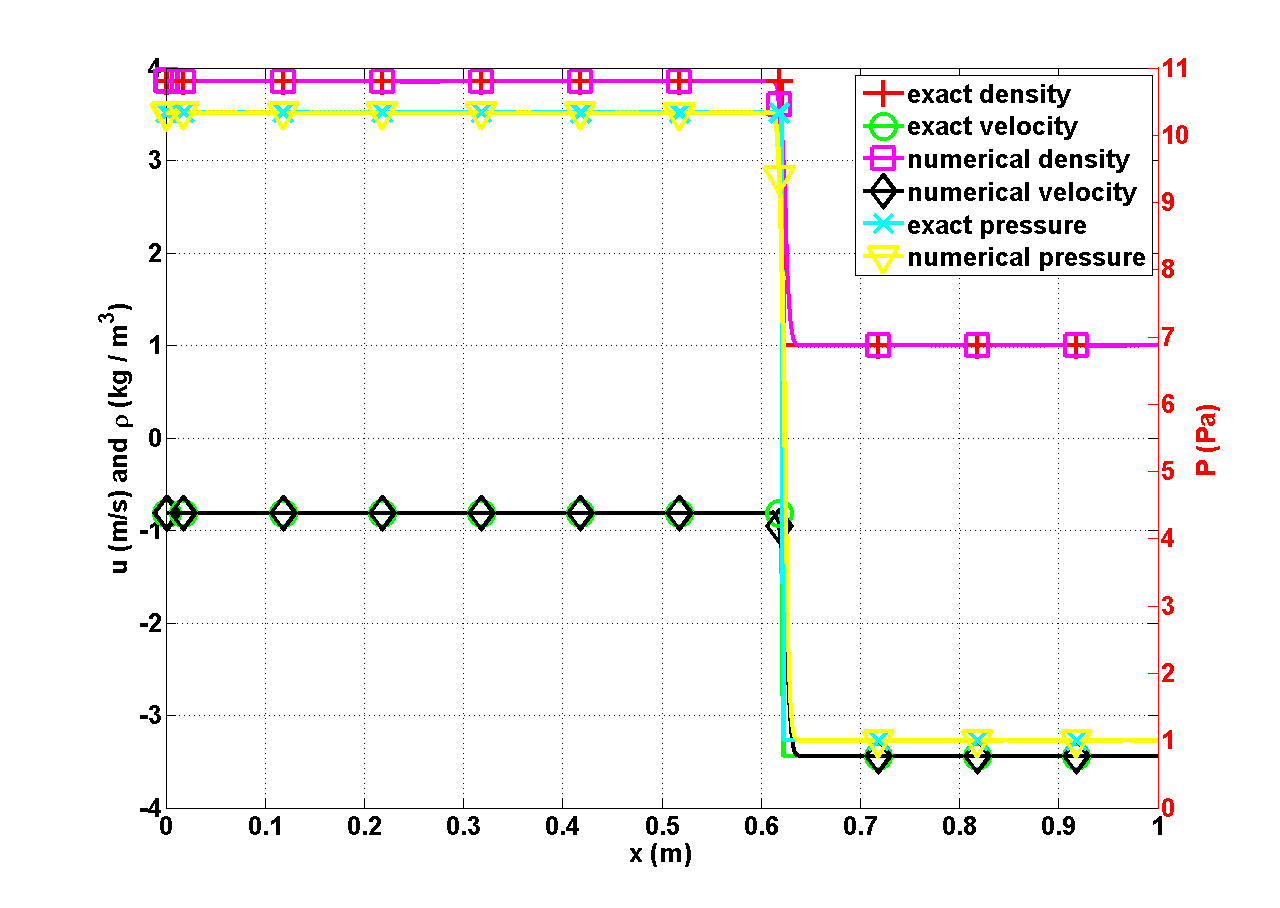
\includegraphics[width=\textwidth]{SlowMovingShock_density_velocity_pressure_profiles.png}
                \caption{Velocity, density and pressure}
                \label{fig:profiles_sms}
        \end{subfigure}%

        \begin{subfigure}[b]{0.495\textwidth}
                \centering
                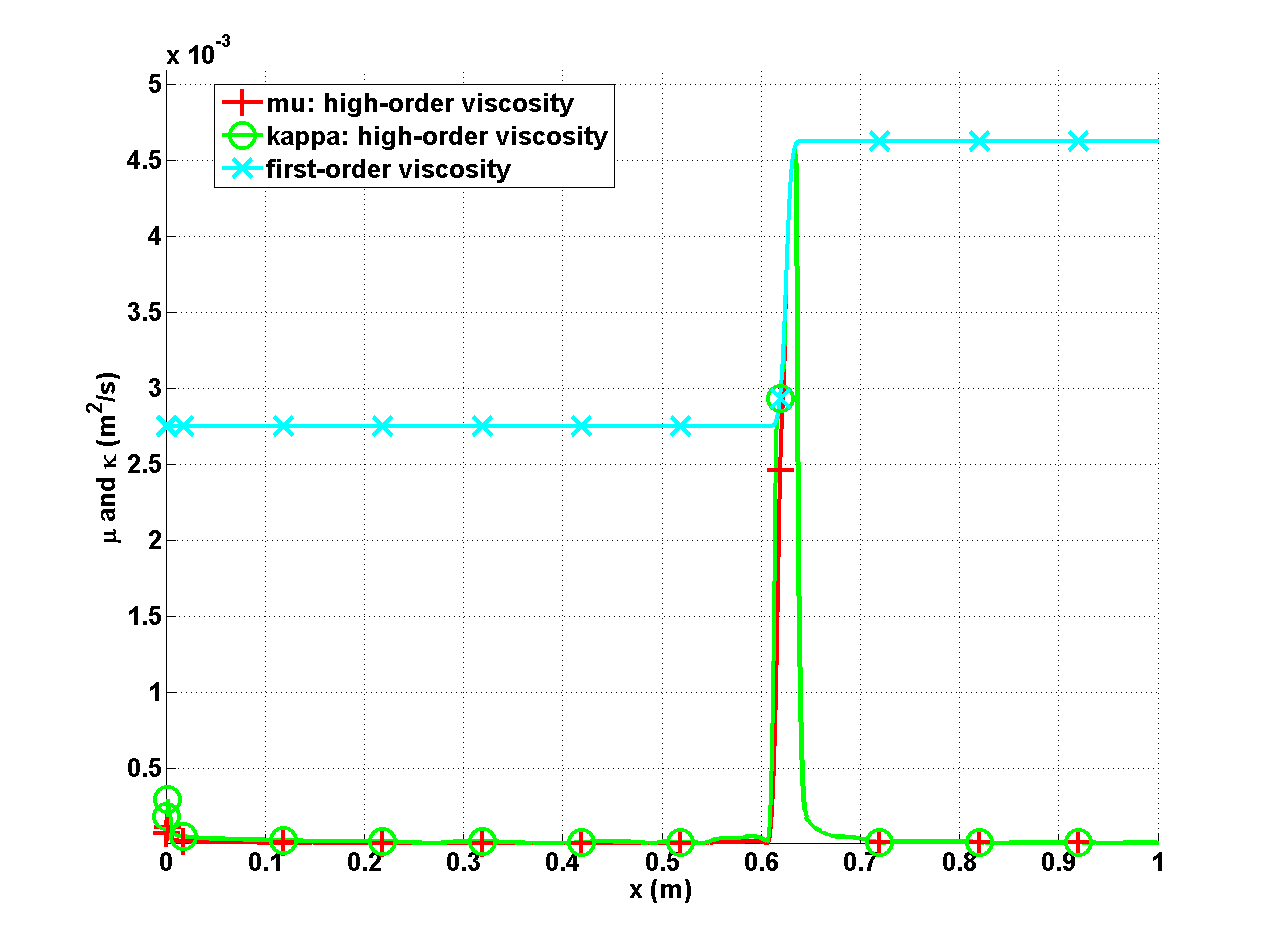
\includegraphics[width=\textwidth]{SlowMovingShock_viscosity.png}
                \caption{Viscosity coefficients}
                \label{fig:viscosity_sms}
        \end{subfigure} 
        \caption{Slow moving shock profiles at $t=1.1s$.}\label{fig:low_moving_shock}
\end{figure} 


%---------------------------------------------------------------------------------------------------
\subsection{Subsonic flow over a 2-D cylinder} \label{sec:cylinder}
%---------------------------------------------------------------------------------------------------

Fluid flow over a 2-D cylinder is often used as a benchmark case to test numerical schemes in the low-Mach regime \cite{LowMach1, LowMach2, LowMach3, guillard}. For this test, an analytical solution is available in the incompressible limit or low-Mach limit and is often referred to as the potential flow solution \tcr{check my change} \tcb{done}. The main features of the potential flow are the following:
%
\begin{itemize}
\item The solution is symmetric: the iso-Mach countour lines are used to asses the symmetry of the numerical solution;
\item The velocity at the top of the cylinder is twice the incoming velocity set at the inlet;
\item The pressure fluctuations are proportional to the square of inlet Mach number, i.e., 
\begin{equation}
\delta P = \frac{\max(P(\vec{r})) - \min(P(\vec{r}))}{\max(P(\vec{r}))}  \propto M_\infty^2
%||\tilde{\vec{u}}|| = \frac{\max(||\vec{u}||) - \min(||\vec{u}||)}{\max(||\vec{u}||)}  \propto M_\infty\nonumber 
\end{equation}
where $\delta P$ and $M_\infty$ denote the pressure fluctuations and the inlet Mach number, respectively.
\end{itemize}
%
The computational domain consists of a $1\times 1$ square with a circular hole of radius $0.05$ in its center. A $\mathbb{P}_1$ triangular mesh with $4008$ triangular elements was used to discretize the geometry. The ideal gas equation of state, with $\gamma=1.4$ is used. At the inlet, a subsonic stagnation boundary condition is used: the stagnation pressure and temperature are computed using the following relations:
%
\begin{equation}
\label{eq:stagnation_relations}
\left\{
\begin{array}{l}
P_0 = P\left( 1 + \frac{\gamma-1}{2} M^2 \right)^{\frac{\gamma-1}{\gamma}} \\
T_0 = T\left( 1 + \frac{\gamma-1}{2} M^2 \right)
\end{array}
\right.
\end{equation}
%
An static pressure boundary condition is used for the outlet boundary and the following static pressure $P_s = 101,325$ $Pa$ is set. The implementation of the pressure boundary conditions is done on the model of \cite{SEM}. A solid wall boundary condition is set for the top and bottom walls of the computational domain: the normal component of the velocity. The simulations are run until a steady-state is reached with a $CFL$ of $40$. The steady-state is reached when the norm of total residual (including all equations) is lower than $10^{-12}$.

Several simulations are performed, with inlet Mach numbers $M_{\text{inlet}}$ ranging from $10^{-3}$ to $10^{-7}$, and are shown in \fig{fig:cylinder}. The iso-Mach contour lines are drawn using $30$ equally-spaced intervals $2 \ 10^{-10}$ to $M_{\text{inlet}}$ and allow us to assess the symmetry of the numerical solution.
%
\begin{figure}[H]
        \centering
        \begin{subfigure}[b]{0.495\textwidth}
                \centering
                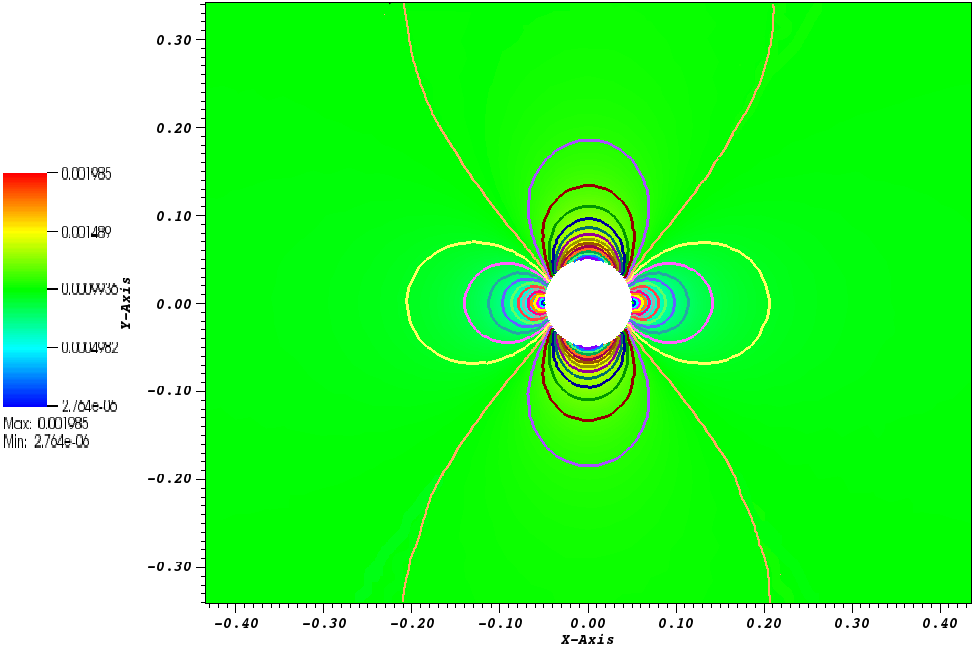
\includegraphics[width=\textwidth]{CylinderMach1em3ZoomIn.png}
                \caption{$M_{\text{inlet}}=10^{-3}$}
                \label{fig:cyl_1em3}
        \end{subfigure}%

        \begin{subfigure}[b]{0.495\textwidth}
                \centering
                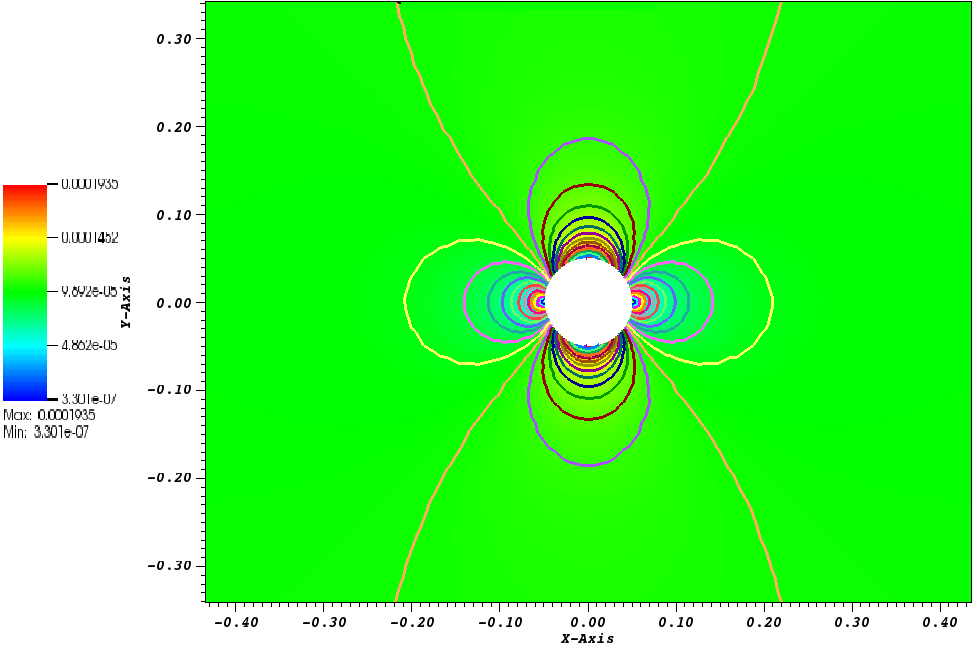
\includegraphics[width=\textwidth]{CylinderMach1em4ZoomIn.png}
                \caption{$M_{\text{inlet}}=10^{-4}$}
                \label{fig:cyl_1em4}
        \end{subfigure}    

        \begin{subfigure}[b]{0.495\textwidth}
                \centering
                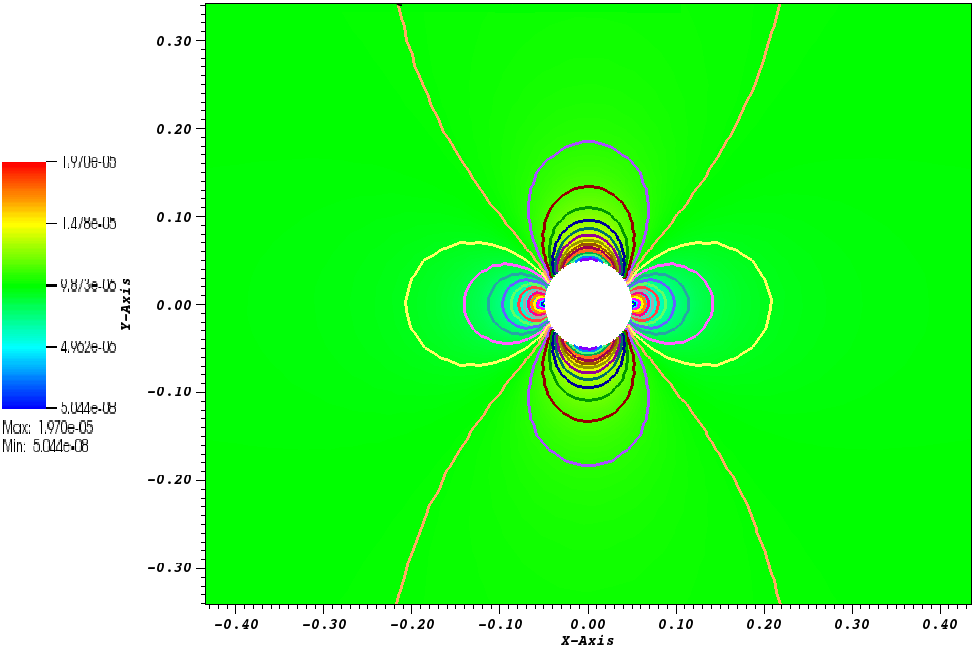
\includegraphics[width=\textwidth]{CylinderMach1em5ZoomIn.png}
                \caption{$M_{\text{inlet}}=10^{-5}$}
                \label{fig:cyl_1em5}
        \end{subfigure}

        \begin{subfigure}[b]{0.495\textwidth}
                \centering
                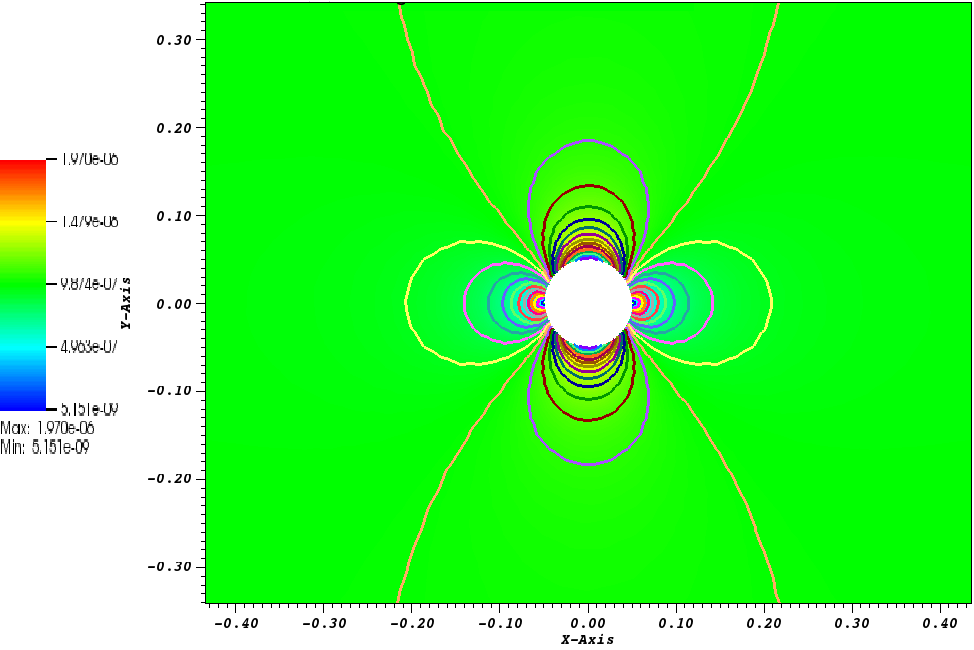
\includegraphics[width=\textwidth]{CylinderMach1em6ZoomIn.png}
                \caption{$M_{\text{inlet}}=10^{-6}$}
                \label{fig:cyl_1em6}
        \end{subfigure}

        \begin{subfigure}[b]{0.495\textwidth}
                \centering
                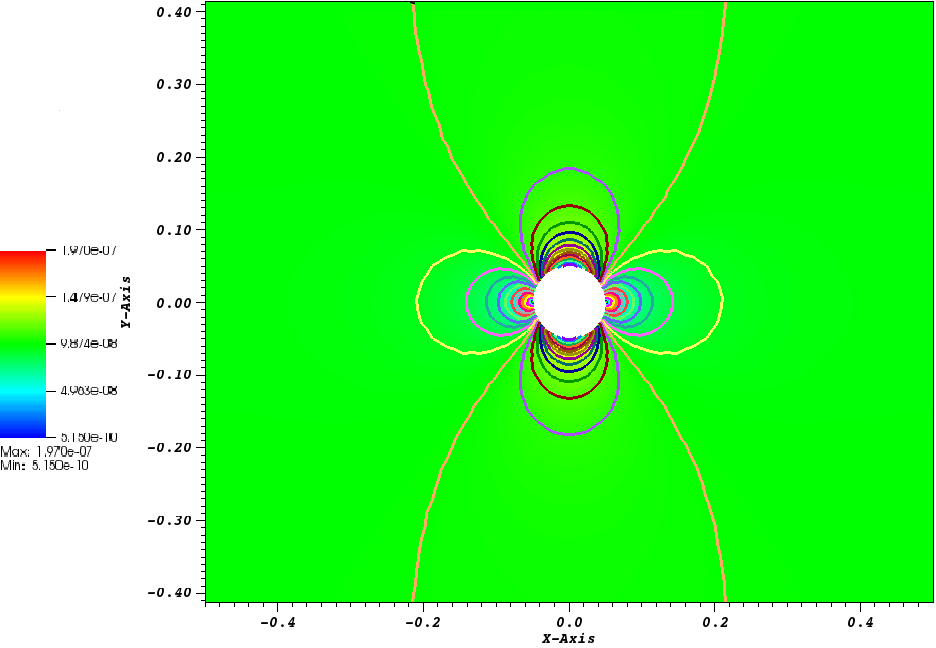
\includegraphics[width=\textwidth]{CylinderMach1em7ZoomIn.png}
                \caption{$M_{\text{inlet}}=10^{-7}$}
                \label{fig:cyl_1em7}
        \end{subfigure}
        \caption{Iso-Mach lines for a subsonic flow over a 2-D cylinder with inlet Mach number values from ranging from $10^{-3}$ to $10^{-7}$ (steady-state solution).}
				\label{fig:cylinder}
\end{figure}
%
The velocity at the top of the cylinder and at the inlet are given for different Mach-number values (ranging from $10^{-3}$ to $10^{-7}$) in \tbl{tbl:velocity_ratio}. The ratio of the inlet velocity to the velocity at the top of cylinder is also computed and is very close to the theoretical value of $2$ that is expected in the incompressible limit \tcr{check my mods} \tcb{I did}.
%
\begin{table}[H]
\begin{center}
 \caption{\label{tbl:velocity_ratio}Velocity ratio for different Mach numbers.}
\begin{tabular}{|c|c|c|c|}
\hline
Mach number & inlet velocity & velocity at the top of the cylinder & ratio \\ \hline
$10^{-3}$ & $2.348$ $10^{-3}$ & $1.176$ $10^{-3}$& $1.99$  \\ \hline
$10^{-4}$ & $2.285$ $10^{-4}$ & $1.145$ $10^{-4}$& $1.99$  \\ \hline
$10^{-5}$ & $2.283$ $10^{-5}$ & $1.144$ $10^{-5}$ & $1.99$ \\ \hline
$10^{-6}$ & $2.283$ $10^{-6}$ & $1.144$ $10^{-6}$ & $1.99$ \\ \hline
$10^{-7}$ & $2.283$ $10^{-7}$ & $1.144$ $10^{-7}$ & $1.99$ \\ \hline
\end{tabular}
\end{center}
\nonumber
\end{table}
%
In \fig{fig:pressure_vel_fluc}, the fluctuations in pressure and velocity are plotted as a function of the Mach number (on a log-log scale). The fluctuations are expected to be of the order of $M^2$ and $M$ for the pressure and velocity, respectively. It is known that some stabilization methods, e.g., \cite{guillard, rajoute'dautres exemples}, can produce pressure fluctuations with the wrong Mach-number order. Here, entropy viscosity method yields the correct order in the low-Mach limit. For easy of comparison, the reference lines with slope values of 1 and 2 are also provided. \tcr{change the legend in the plot appropriately}
%
\begin{figure}[H]
\centering
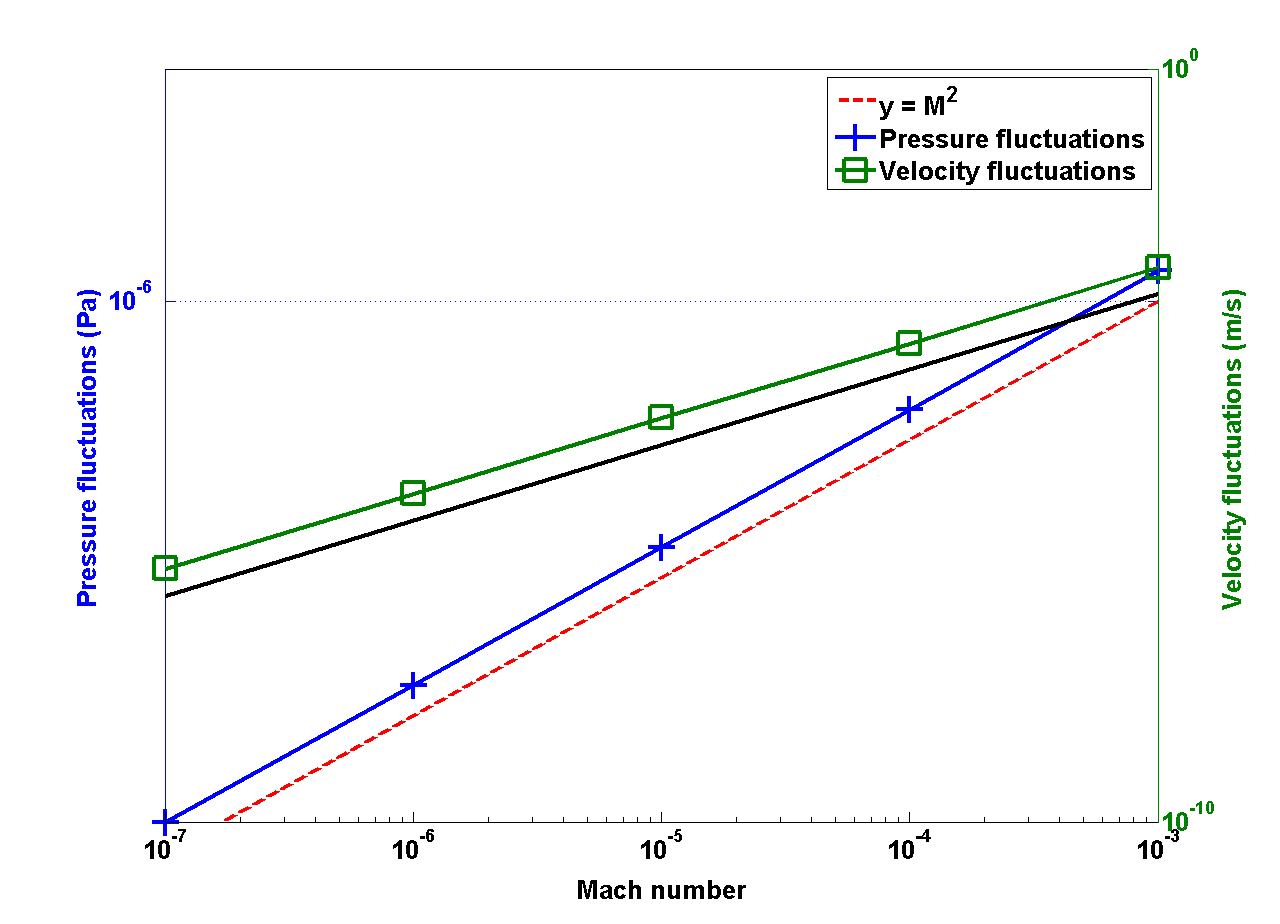
\includegraphics[width=\textwidth]{pressure_fluctuation.png}
\caption{Log-log plot of the pressure and velocity fluctuations as a function of the far-field Mach number.}
\label{fig:pressure_vel_fluc}
\end{figure}

%---------------------------------------------------------------------------------------------------
\subsection{Subsonic flow over a 2-D hump} \label{sec:hump}
%---------------------------------------------------------------------------------------------------

\tcr{Is it a circular hump or Gaussian hump in the literature???}

This is a another example of an internal flow configuration. It consists of a channel of height $L=1$ $m$ and length $3L$, with a circular bump of length $L$ and thickness $0.1L$. The bump is located on the bottom wall at a distance $L$ from the inlet. The system is initialized with an uniform pressure $P=101,325$ $Pa$ and temperature $T=300$ $K$. The initial velocity is computed from the inlet Mach number, the pressure, the temperature and the ideal gas equation (with  $\gamma=1.4$). Here,  $C_v = 717$ $J/kg-K$. At the inlet, a subsonic stagnation boundary condition is used and the stagnation pressure and temperature are computed using \eqt{eq:stagnation_relations}.
The static pressure $P_s = 101,325$ $Pa$ is set at the subsonic outlet. The results are shown in \fig{fig:2d_hump_mach_0p7}, \fig{fig:2d_hump_mach_0p01}, \fig{fig:2d_hump_mach_0p0001} and \fig{fig:2d_hump_mach_0p0000001} for the inlet Mach numbers $M_{\infty}=0.7$, $M_{\infty}=0.01$, $M_{\infty}=10^{-4}$ and $M_{\infty}=10^{-7}$, respectively. It is expected that, within the low Mach number range, the solution does not depend on the Mach number and is identical to the solution obtained with an incompressible flow code. On the other hand, for a flow at $M=0.7$, the compressible effects become more important and shock can form. An uniform grid of $3352$ $Q_1$ elements was used to obtain the numerical solution for Mach numbers below $M_{\infty}=0.01$. A once-refined mesh was employed for the $M_{\infty}=0.7$ simulation in order to better resolve the shock. A $CFL$ of $20$ was employed and the simulations were run until steady state.
%
\begin{figure}[H]
        \centering
        \begin{subfigure}[b]{0.5\textwidth}
                \centering
                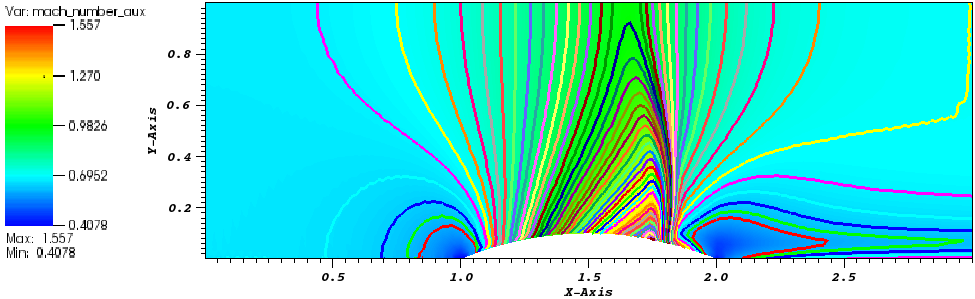
\includegraphics[width=\textwidth]{Hump2D_mach_0p7.png}
                \caption{Mach $0.7$}
                \label{fig:2d_hump_mach_0p7}
        \end{subfigure}%

        \begin{subfigure}[b]{0.5\textwidth}
                \centering
                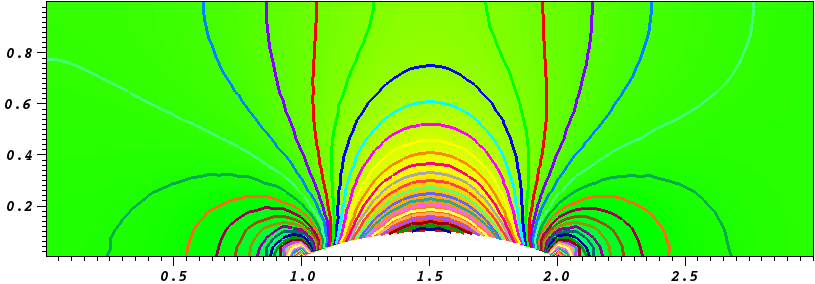
\includegraphics[width=\textwidth]{Hump2D_mach_0p01.png}
                \caption{Mach $10^{-2}$}
                \label{fig:2d_hump_mach_0p01}
        \end{subfigure}%
        
        \begin{subfigure}[b]{0.495\textwidth}
                \centering
                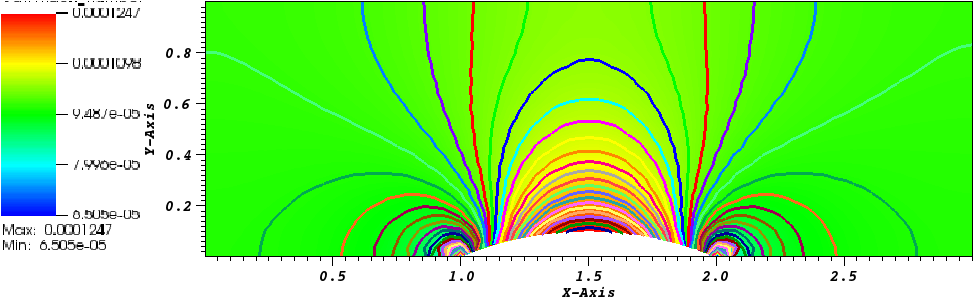
\includegraphics[width=\textwidth]{Hump2D_mach_1em4.png}
                \caption{Mach $10^{-5}$}
                \label{fig:2d_hump_mach_0p0001}
        \end{subfigure}

        \begin{subfigure}[b]{0.495\textwidth}
                \centering
                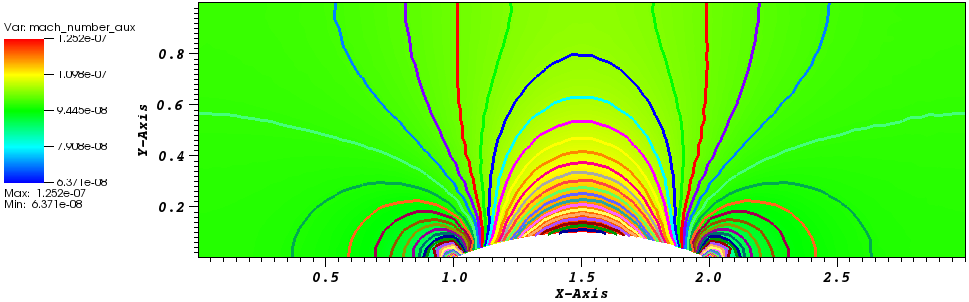
\includegraphics[width=\textwidth]{Hump2D_mach_1em7.png}
                \caption{Mach $10^{-7}$}
                \label{fig:2d_hump_mach_0p0000001}
        \end{subfigure}
        \caption{Iso-Mach lines for a 2-D flow over a circular bump (steady-state solution).}
				\label{fig:2d_hump}
\end{figure}
%
The results showed in \fig{fig:2d_hump_mach_0p01}, \fig{fig:2d_hump_mach_0p0001} and \fig{fig:2d_hump_mach_0p0000001} correspond to the low-Mach regime. The iso-Mach lines are drawn ranging from the minimum and the maximum values (provided in each legend) using 50 equally-spaced intervals. The steady-state solution is symmetric and does not depend on the value of the inlet Mach number, as expected in the incompressible limit. 

In \fig{fig:2d_hump_mach_0p7}, the steady-state numerical solution develops a shock: the compressibility effect are no longer negligible. The iso-Mach lines are also plotted with $50$ intervals and range from $0.4$ to $1.6$. The shock is well resolved and does not display any instabilities or spurious oscillations. \\
The results presented in \fig{fig:2d_hump} were obtained with the new definitions of the viscosity coefficients and illustrate the ability of the entropy viscosity method to correctly simulate several types of flows (subsonic and transonic flows) without tuning parameters.

%---------------------------------------------------------------------------------------------------
\subsection{Supersonic flow in a compression corner} \label{sec:corner}
%---------------------------------------------------------------------------------------------------

In this last example, we consider a supersonic flow at Mach 2.5 impinging on a corner with an angle of $15^\circ$. From the oblique shock theory \cite{CompressionCorner}, an analytical solution for this supersonic flow is available and give the downstream to upstream pressure, entropy and Mach number ratios. 
The initial conditions are chosen to be spatially uniform: the pressure and temperature are set to $P=101,325$ $Pa$ and $T=300$ $K$, respectively.  The ideal gas equation of state is used with the same parameters as in \sct{sec:hump}. The initial velocity is computed from the upstream Mach number. The inlet is supersonic and therefore, the pressure, temperature and velocity are specified using Dirichlet boundary conditions. The outlet is also supersonic and none of the characteristics enter the domain through this boundary: the values will be computed by the implicit solver.

The simulation is run with $CFL=2$, until steady state is reached. A 2-D mesh made of $16,109$ $\mathbb{Q}_1$ elements is used. The ratios for pressure, entropy and Mach number computed using the  analytical and the numerical solutions are given in \tbl{tbl:corner_exact_sol}; they are in excellent agreement. The shock wave angle at steady state is also known and given by the so-called $\theta -\beta -M$ relation:
%
\begin{equation}
\tan \theta = 2 \cot \beta \frac{M^2 \sin^2 \beta -1}{M^2 \left(\gamma+\cos^2 (2\beta)\right)+2} ,
\end{equation}
%
where $\theta$, $\beta$ and $M$ denote the corner angle, the shock wave angle, and the upstream Mach number, respectively. For Mach 2.5 and a 15$^\circ$ corner angle, the analytical value for the shock wave angle is $36.94^{\circ}$ at steady-state. From \fig{fig:2d_corner_mach}, the numerical value of the shock wave angle can be measured and is found to be equal to $36.9^{\circ}$, and thus in excellent agreement with theory.
%
\begin{table}[H]
\begin{center}
\begin{tabular}{|c|c|c|}  \hline
            & analytical & numerical\\ \hline
Pressure    & 2.47       & 2.47   \\ \hline
Mach number &  0.74      & 0.74    \\ \hline
Entropy     & 1.03       & 1.03    \\ \hline 
\end{tabular}
\caption{\label{tbl:corner_exact_sol} Ratio of analytical and numerical downstream to upstream quantities for the compression corner problems (corner angle of $15^\circ$ and inlet $M=2.5$.}
\end{center}
\end{table}
%
\begin{figure}[H]
        \centering
        \begin{subfigure}[b]{0.52\textwidth}
                \centering
                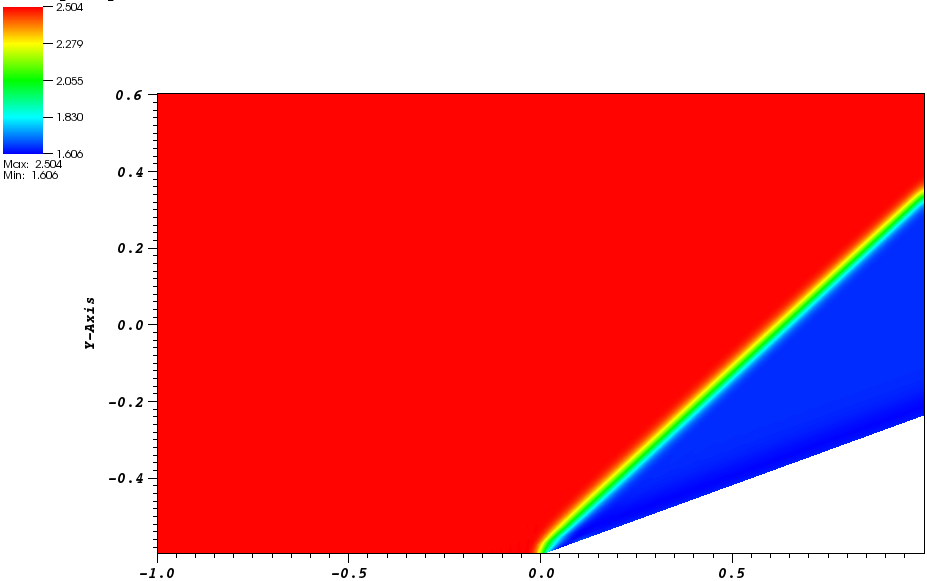
\includegraphics[width=\textwidth]{CompressionCorner2D_mach.png}
                \caption{Mach number}
                \label{fig:2d_corner_mach}
        \end{subfigure}%

        \begin{subfigure}[b]{0.52\textwidth}
                \centering
                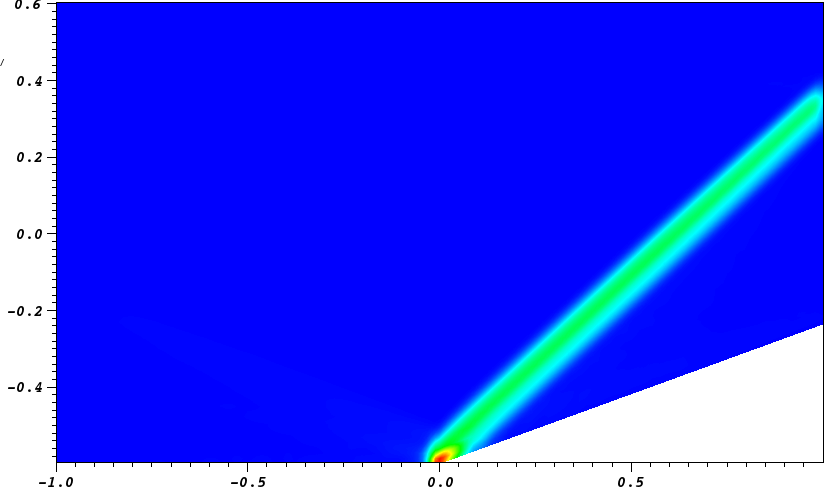
\includegraphics[width=\textwidth]{CompressionCorner2D_viscosity.png}
                \caption{Viscosity coefficients}
                \label{fig:2d_corner_visc}
        \end{subfigure}
        
        \begin{subfigure}[b]{0.49\textwidth}
                \centering
                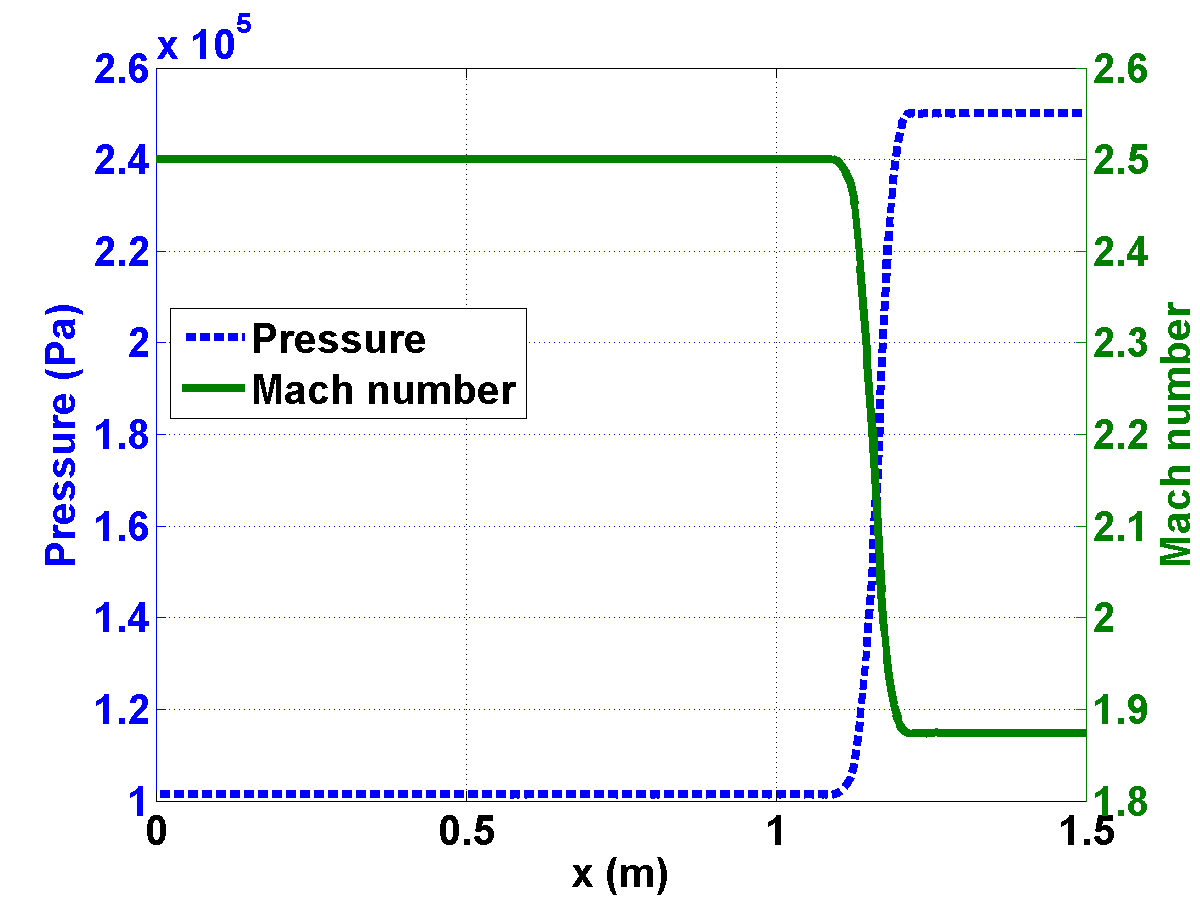
\includegraphics[width=\textwidth]{mach_number_pressure.png}
                \caption{Pressure and Mach number}
                \label{fig:2d_corner_isomach}
        \end{subfigure}        

        \begin{subfigure}[b]{0.49\textwidth}
                \centering
                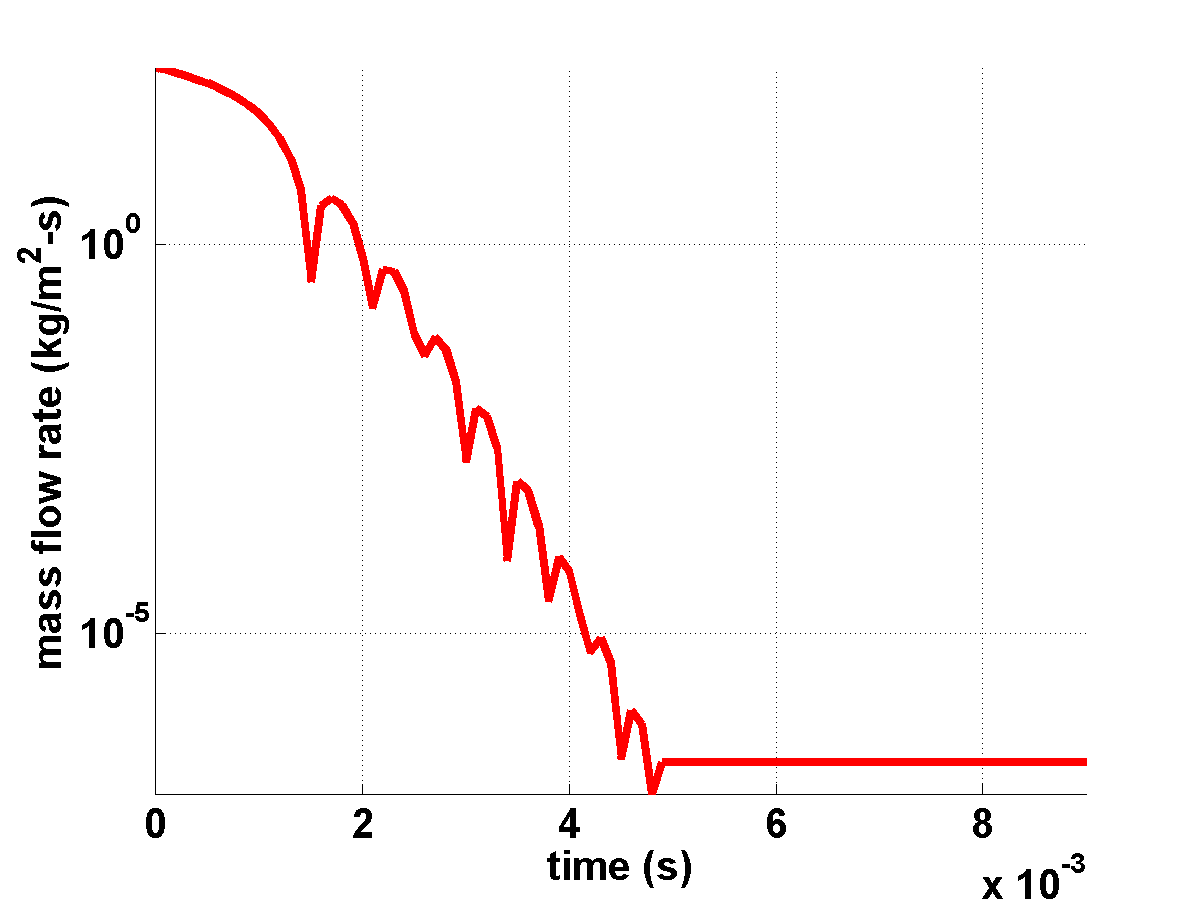
\includegraphics[width=\textwidth]{CompressionCorner2DQ.png}
                \caption{Difference between inlet and outlet mass flow rates as a function of time.}
                \label{fig:2d_convergence}
        \end{subfigure}
        \caption{Steady-state solution for a flow in a 2-D compression corner.}\label{fig:2d_corner}
\end{figure}
%
The steady-state numerical solution is given in \fig{fig:2d_corner}: the Mach number and the viscosity coefficients are plotted in \fig{fig:2d_corner_mach} and \fig{fig:2d_corner_visc}, respectively. The steady-state solution is formed of two regions of constant states, separated by the oblique shock. \fig{fig:2d_corner_visc} shows that the viscosity coefficient is large in the shock and small elsewhere, as expected. At the location of the corner ($x=-0.25m$, $y=-0.5m$), the viscosity coefficient is peaked because of the treatment of the wall boundary condition: at this particular node, the normal is not well defined and may cause some numerical errors. The 1-D graphs at $y=0$ for the pressure and the Mach number are given in \fig{fig:2d_corner_isomach}: no spurious oscillations are observed and the shock is well resolved. Finally, the difference between the inlet and outlet mass flow rates is plotted in \fig{fig:2d_convergence} which shows that the steady state is reached. 

%%%%%%%%%%%%%%%%%%%%%%%%%%%%%%%%%%%%%%%%%%%%%%%%%%%%%%%%%%%%%%%%%%%%%%%%%%%%%%%%%%%%%%%%%%%%%%%%%%%%
%%%%%%%%%%%%%%%%%%%%%%%%%%%%%%%%%%%%%%%%%%%%%%%%%%%%%%%%%%%%%%%%%%%%%%%%%%%%%%%%%%%%%%%%%%%%%%%%%%%%
\section{Conclusions} \label{sec:ccl}
%%%%%%%%%%%%%%%%%%%%%%%%%%%%%%%%%%%%%%%%%%%%%%%%%%%%%%%%%%%%%%%%%%%%%%%%%%%%%%%%%%%%%%%%%%%%%%%%%%%%
%%%%%%%%%%%%%%%%%%%%%%%%%%%%%%%%%%%%%%%%%%%%%%%%%%%%%%%%%%%%%%%%%%%%%%%%%%%%%%%%%%%%%%%%%%%%%%%%%%%%

A new version of the entropy viscosity method valid for a wide range of Mach number and applied to the multi-D Euler equations with variable area was derived and presented. The definition of the viscosity coefficient is now consistent with the low Mach asymptotic limit, does not require an analytical expression of the entropy function, and thus, could be used with any equation of state having a convex entropy. Tests were performed with the Ideal and Stiffened Gas equation of states. In 1-D, convergence of the numerical solution (either smooth or with shocks) to the exact solution was demonstrated by computing the convergence rates of the L$1$ and L$2$ norms of the error for flows in convergence-divergent nozzle and a straight pipe. 2-D simulations were also performed for both subsonic and supersonic flows, and various geometries: the entropy viscosity method behaves well for a wide range of Mach number. The numerical results obtained for a flow over a circular bump (subsonic and transonic flows) illustrates the capabilities of the method to adapt to the flow type. \\
As future work, the entropy viscosity method will be extended to the 1-D seven equations model \cite{SEM}. This two-phase flow system of equations is a good candidate for two reasons: it is unconditionally hyperbolic and degenerates to the multi-D Euler equations when one phase disappears.

%%%%%%%%%%%%%%%%%%%%%%%%%%%%%%%%%%%%%%%%%%%%%%%%%%%%%%%%%%%%%%%%%%%%%%%%%%%%%%%%%%%%%%%%%%%%%%%%%%%%
%%%%%%%%%%%%%%%%%%%%%%%%%%%%%%%%%%%%%%%%%%%%%%%%%%%%%%%%%%%%%%%%%%%%%%%%%%%%%%%%%%%%%%%%%%%%%%%%%%%%

%%%%%%%%%%%%%%%%%%%%%%%%%%%%%%%%%%%%%%%%%%%%%%%%%%%%%%%%%%%%%%%%%%%%%%%%%%%%%%%%%%%%%%%%%%%%%%%%%%%%
%%%%%%%%%%%%%%%%%%%%%%%%%%%%%%%%%%%%%%%%%%%%%%%%%%%%%%%%%%%%%%%%%%%%%%%%%%%%%%%%%%%%%%%%%%%%%%%%%%%%
\section*{Acknowledgments} 
The authors would like to thank Bojan Popov and Jean-Luc Guermond for many fruitful discussions.  

%%%%%%%%%%%%%%%%%%%%%%%%%%%%%%%%%%%%%%%%%%%%%%%%%%%%%%%%%%%%%%%%%%%%%%%%%%%%%%%%%%%%%%%%%%%%%%%%%%%%
%%%%%%%%%%%%%%%%%%%%%%%%%%%%%%%%%%%%%%%%%%%%%%%%%%%%%%%%%%%%%%%%%%%%%%%%%%%%%%%%%%%%%%%%%%%%%%%%%%%%
\bibliography{mybibfile}
%%%%%%%%%%%%%%%%%%%%%%%%%%%%%%%%%%%%%%%%%%%%%%%%%%%%%%%%%%%%%%%%%%%%%%%%%%%%%%%%%%%%%%%%%%%%%%%%%%%%
%%%%%%%%%%%%%%%%%%%%%%%%%%%%%%%%%%%%%%%%%%%%%%%%%%%%%%%%%%%%%%%%%%%%%%%%%%%%%%%%%%%%%%%%%%%%%%%%%%%%
\newpage
%%%%%%%%%%%%%%%%%%%%%%%%%%%%%%%%%%%%%%%%%%%%%%%%%%%%%%%%%%%%%%%%%%%%%%%%%%%%%%%%%%%%%%%%%%%%%%%%%%%%
%%%%%%%%%%%%%%%%%%%%%%%%%%%%%%%%%%%%%%%%%%%%%%%%%%%%%%%%%%%%%%%%%%%%%%%%%%%%%%%%%%%%%%%%%%%%%%%%%%%%
\appendix
%%%%%%%%%%%%%%%%%%%%%%%%%%%%%%%%%%%%%%%%%%%%%%%%%%%%%%%%%%%%%%%%%%%%%%%%%%%%%%%%%%%%%%%%%%%%%%%%%%%%
%%%%%%%%%%%%%%%%%%%%%%%%%%%%%%%%%%%%%%%%%%%%%%%%%%%%%%%%%%%%%%%%%%%%%%%%%%%%%%%%%%%%%%%%%%%%%%%%%%%%

%%%%%%%%%%%%%%%%%%%%%%%%%%%%%%%%%%%%%%%%%%%%%%%%%%%%%%%%%%%%%%%%%%%%%%%%%%%%%%%%%%%%%%%%%%%%%%%%%%%%
%%%%%%%%%%%%%%%%%%%%%%%%%%%%%%%%%%%%%%%%%%%%%%%%%%%%%%%%%%%%%%%%%%%%%%%%%%%%%%%%%%%%%%%%%%%%%%%%%%%%
\section{Derivation of the entropy residual as a function of density, pressure and speed of sound} \label{app:ent_res}
%%%%%%%%%%%%%%%%%%%%%%%%%%%%%%%%%%%%%%%%%%%%%%%%%%%%%%%%%%%%%%%%%%%%%%%%%%%%%%%%%%%%%%%%%%%%%%%%%%%%
%%%%%%%%%%%%%%%%%%%%%%%%%%%%%%%%%%%%%%%%%%%%%%%%%%%%%%%%%%%%%%%%%%%%%%%%%%%%%%%%%%%%%%%%%%%%%%%%%%%%

The entropy residual is as follows:
%
\begin{equation*}
\resi(\vec{r},t) = \partial_t s (\vec{r},t) + \vec{u} \cdot \div s (\vec{r},t) ,
\end{equation*}
%
where all variables were defined previously. This form of the entropy residual is not suitable for the low-Mach limit as explained in \sct{sec:background}. In this appendix, we recast the entropy residual $\resi(\vec{r},t)$ as a function of the primitive variables (pressure, velocity and density) and the speed of sound. The first step of this derivation is to use the chain rule, recalling that the entropy is a function of the internal energy $e$ and the density $\rho$, yielding
%
\begin{equation*}
\resi(\vec{r},t) = s_e  \matder{e} + s_{\rho}  \matder{\rho} ,
\end{equation*}
%
where $s_e$ denotes the partial derivative of $s$ with respect to the variable $e$. We recall that $\matder{\ }$ denotes the material derivative. Since the internal energy $e$ is a function of pressure $P$ and density $\rho$ (through the equation of state), we use again the chain rule to re-express the previous equation as a function of of the material derivatives in $P$ and $\rho$:
%
\begin{eqnarray*}
\resi(\vec{r},t) &=&  s_e e_P \matder{P} + ( s_e e_{\rho} + s_{\rho} ) \matder{\rho} \\
&=& s_e e_P \left( \matder{P} + \frac{1}{s_e e_P} ( s_e e_{\rho} + s_{\rho} )  \matder{\rho}\right) \\
&=& s_e e_P \left( \matder{P} + ( \frac{e_{\rho}}{e_P} + \frac{s_{\rho}}{s_e e_P} )  \matder{\rho} \right) .
\end{eqnarray*}
%
We are now close to the final result (see \eqt{eq:ent_res}). To prove that the term multiplying the material derivative of the density is indeed equal to the square of the speed of sound, we recall that the speed of sound is defined as the partial derivative of pressure with respect to density at constant entropy, which can be recast as a function of the entropy as follows (see Appendix A.2 of \cite{jlg}):
%
\begin{equation*}
c^2 := \left. \frac{\partial P}{\partial \rho} \right|_{s=cst} = P_{\rho} - \frac{s_{\rho}}{s_e} P_e   \, .
\end{equation*}
%
Using the following relations (see Appendix A.1 of \cite{jlg})
%
\begin{equation*}
P_e = \frac{1}{e_P} \text{ and } P_{\rho} = -\frac{e_{\rho}}{e_P}  \, ,
\end{equation*}
%
\eqt{eq:ent_res} is obtained and recalled below for completeness:
%
\begin{equation*}
\resi(\vec{r},t) := \partial_t s + \vec{u} \cdot \grad s = \matder{s} = \frac{s_e}{P_e} \left( \underbrace{\matder{P} - c^2 \matder{\rho} }_{\resinew(\vec{r},t)} \right) \, .
\end{equation*} 

%%%%%%%%%%%%%%%%%%%%%%%%%%%%%%%%%%%%%%%%%%%%%%%%%%%%%%%%%%%%%%%%%%%%%%%%%%%%%%%%%%
\newpage
%%%%%%%%%%%%%%%%%%%%%%%%%%%%%%%%%%%%%%%%%%%%%%%%%%%%%%%%%%%%%%%%%%%%%%%%%%%%%%%%%%%%%%%%%%%%%%%%%%%%
%%%%%%%%%%%%%%%%%%%%%%%%%%%%%%%%%%%%%%%%%%%%%%%%%%%%%%%%%%%%%%%%%%%%%%%%%%%%%%%%%%%%%%%%%%%%%%%%%%%%
\section{Derivation of the dissipative terms for the Euler equations with variable area using the entropy minimum principle} \label{app:diss_terms}
%%%%%%%%%%%%%%%%%%%%%%%%%%%%%%%%%%%%%%%%%%%%%%%%%%%%%%%%%%%%%%%%%%%%%%%%%%%%%%%%%%%%%%%%%%%%%%%%%%%%
%%%%%%%%%%%%%%%%%%%%%%%%%%%%%%%%%%%%%%%%%%%%%%%%%%%%%%%%%%%%%%%%%%%%%%%%%%%%%%%%%%%%%%%%%%%%%%%%%%%%
%
Euler equations (without viscous regularization) with variable area are recalled here
%
\begin{subequations}
\label{app:euler_variable_A}
%
\begin{equation}
\partial_t \left( \rho A \right) + \div \left( \rho \vec{u} A \right) = 0 
\end{equation}
%
\begin{equation}
\partial_t \left( \rho \vec{u} A \right) + \div \left[A\left( \rho \vec{u} \otimes \vec{u} + P \mathbf{I} \right) \right] = P \grad A 
\end{equation}
% 
\begin{equation}
\partial_t \left( \rho E A \right) + \div \left[ \vec{u} A \left( \rho E + P \right) \right] = 0 \,.
\end{equation}
\end{subequations}
%
The specific entropy is assumed \tcr{can it be depend on other variables?} to be a function of the density $\rho$ and the internal energy $e$, i.e., $s(e,\rho)$ , the above system of equations satisfies the minimum entropy principle \cite{Toro} \tcr{is this really shown in Toro?}
%
\begin{equation}
A \rho \left( \partial_t s + \vec{u} \cdot \div s \right) \geq 0 \, .
\end{equation}
%
The entropy function $s$ satisfies the second law of thermodynamics, $T ds = de - \frac{P}{\rho^2} d \rho$, which implies $s_e := T^{-1}$ and $s_\rho := -P T^{-1} \rho^{-2}$. One can show that \cite{guermond popow theoretical paper}
%
\begin{equation}
s_e = T^{-1} \geq 0 \text{ and }
Ps_e + \rho^2 s_{\rho} 
\end{equation}
%
In order to apply the entropy viscosity method to the variable-area Euler equations, dissipative terms need to be added to each equation in \eqt{app:euler_variable_A}. The functional forms of these terms need to be such that the entropy residual derived with these terms present also satisfies the minimum entropy principle. 
%By inspecting the extra terms that will appear in the entropy residual, due to the dissipative terms will appear in the left-hand side. 
To prove the minimum entropy principle, the extra terms appearing in the entropy residual are either recast as conservative terms or shown to be positive. The rest of this appendix presents this demonstration. 
Following \cite{guermond popow theoretical paper}, we first write the variable-area equation with dissipative terms. 
%
%
\begin{subequations}
\label{app:euler_variable_A_diss}
%
\begin{equation}
\partial_t \left( \rho A \right) + \div \left( \rho \vec{u} A \right) = \div f 
\end{equation}
%
\begin{equation}
\partial_t \left( \rho \vec{u} A \right) + \div \left[A\left( \rho \vec{u} \otimes \vec{u} + P \mathbf{I} \right) \right] = P \grad A + \div g
\end{equation}
% 
\begin{equation}
\partial_t \left( \rho E A \right) + \div \left[ \vec{u} A \left( \rho E + P \right) \right] = \div h \,.
\end{equation}
\end{subequations}
%
where $f$, $g$ and $h$ are dissipative fluxes to be determined. Starting from the modified system of equations given in \eqt{app:euler_variable_A_diss}, the entropy residual is derived again. The derivation requires the following steps : express the governing laws in terms of primitive variables $(\rho, \vec{u}, e)$, multiply the continuity equation by $\rho s_\rho$ and the internal energy equation by $s_e$, and invoke multivariate chain rule, e.g., $\partial s /\partial x = s_e \partial e /\partial x + s_\rho \partial \rho /\partial x$. These steps are similar to the ones form the standard Euler equations \cite{guermond popow theoretical paper}. Some of the lengthy algebra is omitted here. The above steps yield:
%
\begin{multline}
\label{eq:ent_res_app}
A \rho \left( \partial_t s + \vec{u} \cdot \grad s \right) = s_e \left[ \div h + g : \grad u + \left( \frac{u^2}{2}-e \right) \div f \right] 
+ \rho s_{\rho} \div f
\end{multline}
%
The next step consists of choosing a definition for each of the dissipative terms so that the left hand-side is positive. The right hand-side of \eqt{eq:ent_res_app} can be simplified using the following relations, $g = A \mu \grad^s \vec{u} + \vec{u} \otimes f$ and $h = \tilde{h} + \vec{u} \cdot g - 0.5 || \vec{u} ||^2 f$, which yields:
\tcr{I can't get the equation below from the one before with your definitions of h,g,f}
%
\begin{eqnarray}
\label{eq:ent_res_app2}
A \rho \left( \partial_t s + \vec{u} \cdot \div s \right) &=& s_e \left[ \div \tilde{h}-e \div f \right] + \rho s_{\rho} \div f  + A s_e \mu \grad \vec{u}^s : \grad \vec{u}\nonumber
\end{eqnarray}
%
The right hand-side is now integrated by parts:
%
\begin{eqnarray}
\label{eq:ent_res_app3}
A \rho \left( \partial_t s + \vec{u} \cdot \div s \right) &=& \div \left[ s_e \tilde{h}-s_e e f  + \rho s_{\rho} f \right] -\nonumber \\
\div \tilde{h} \grad s_e  &-& f \cdot \grad (e s_e) -  f \cdot \grad ( \rho s_{\rho} ) + A s_e \mu \grad^s \vec{u} : \grad \vec{u} \nonumber
\end{eqnarray}
%
where $\grad^s$ is the symmetric gradient. The term $A s_e \mu \grad^s \vec{u} : \grad \vec{u}$ is positive and thus, does not need any further modification. It %
remains to treat the other terms of the right hand-side that we now call $rhs$:
%
\begin{equation}
rhs = \div \left[ s_e \tilde{h}-s_e e f  + \rho s_{\rho} f \right] - \tilde{h} \cdot \grad s_e  - f \cdot \grad (e s_e) - f \cdot \grad ( \rho s_{\rho} ) \nonumber
\end{equation}
%
The first term of $rhs$ is a conservative terms. By choosing carefully a definition for $\tilde{h}$ and $f$, the conservative term can be expressed as a function of the entropy $s$. It is also required to include the variable area in the choice of the dissipative terms so that when assuming constant area, the regular multi-D Euler equations are recovered. The following definitions for $\tilde{h}$ and $f$ are chosen:
%
\begin{equation}
\tilde{h} = A \kappa \grad ( \rho e ) \text{ and } f = A \kappa \grad \rho, \nonumber 
\end{equation}
%
which yields, using the chain rule:
%
\begin{equation}
rhs = \div (\rho A \kappa \grad s ) - A \kappa \underbrace{\left[ \grad (\rho e) \grad s_e  + \grad \rho \grad (e s_e) +  \grad \rho \grad ( \rho s_{\rho} )  \right]}_{\mathbf{Q}} \nonumber
\end{equation}
%
It remains to treat the term $\mathbf{Q}$ that can be recast under a quadratic form, following the work done in \cite{jlg}:
%
\begin{eqnarray}
\mathbf{Q} &=& X^t \Sigma X \nonumber \\
\text{with } X &=& \begin{bmatrix}
\grad \rho \\
\grad e 
\end{bmatrix}
\text{and } \Sigma = \begin{bmatrix}
       \partial_{\rho} (\rho^2 \partial_{\rho} s) & \partial_{\rho,e} s  \\[0.3em]
       \partial_{\rho,e} s & \partial_{e,e} s           \\[0.3em]
     \end{bmatrix} \nonumber 
\end{eqnarray}
%
The matrix $\Sigma$ is symmetric and identical to the matrix obtained in \cite{jlg}. The sign of the quadratic form can be simply determined by studying the positiveness of the matrix $\Sigma$. In this particular case, it is required to prove that the matrix is negative definite: the quadratic form is in the right hand-side and is preceded of a negative sign. According to \cite{jlg}, the convexity of the opposite of the entropy function $s$ with respect to the internal energy $e$ and the specific volume $1/ \rho$ is sufficient to ensure that the matrix $\Sigma$ is negative definite. \\
Thus, the right hand-side of the entropy residual \eqt{eq:ent_res_app}, are now either recast as conservative terms, or known to be positive. Following the work done by \cite{jlg}, the entropy minimum principle holds.

%%%%%%%%%%%%%%%%%%%%%%%%%%%%%%%%%%%%%%%%%%%%%%%%%%%%%%%%%%%%%%%%%%%%%%%%%%%%%%%%%%
\newpage
%%%%%%%%%%%%%%%%%%%%%%%%%%%%%%%%%%%%%%%%%%%%%%%%%%%%%%%%%%%%%%%%%%%%%%%%%%%%%%%%%%%%%%%%%%%%%%%%%%%%
%%%%%%%%%%%%%%%%%%%%%%%%%%%%%%%%%%%%%%%%%%%%%%%%%%%%%%%%%%%%%%%%%%%%%%%%%%%%%%%%%%%%%%%%%%%%%%%%%%%%
\section{Entropy residual with an isentropic equations of state:} \label{app:ise_equ}
%%%%%%%%%%%%%%%%%%%%%%%%%%%%%%%%%%%%%%%%%%%%%%%%%%%%%%%%%%%%%%%%%%%%%%%%%%%%%%%%%%%%%%%%%%%%%%%%%%%%
%%%%%%%%%%%%%%%%%%%%%%%%%%%%%%%%%%%%%%%%%%%%%%%%%%%%%%%%%%%%%%%%%%%%%%%%%%%%%%%%%%%%%%%%%%%%%%%%%%%%

This appendix aims at showing that the entropy residual is null when assuming an isentropic flow. \\
The entropy residual as a function of the pressure, the density, the velocity and the speed of sound is recalled here:
%
\begin{equation}\label{eq:app_entr}
\resinew = \frac{dP}{dt} - c^2 \frac{d \rho}{dt}
\end{equation}
%
Assuming an isentropic flow, the pressure is only a function of the density as follows: $P = f( \rho )$ or $\rho = f^{-1}( P )$. Using the definition of the speed of sound $c^2 = \left. \frac{\partial P}{\partial \rho} \right)_s$ and the above form the equation of state, the following relation is derived:
%
\begin{equation}\label{eq:app_sp}
c^2 = \left. \frac{\partial P}{\partial \rho} \right)_s = \frac{d P}{d \rho} = \frac{d f(\rho)}{d \rho}
\end{equation}
%
Using the chain rule, the entropy residual of \eqt{eq:app_entr} can be recast as a function of the density, the velocity and the speed of sound, and proven equal to zero:
%
\begin{eqnarray*}
\resinew &=& \frac{d f(\rho)}{d \rho} \frac{d\rho}{dt} - c^2 \frac{d \rho}{dt} \\
\resinew &=& c^2 \frac{d\rho}{dt} - c^2 \frac{d \rho}{dt} \\
\resinew &=&  0 
\end{eqnarray*}

%%%%%%%%%%%%%%%%%%%%%%%%%%%%%%%%%%%%%%%%%%%%%%%%%%%%%%%%%%%%%%%%%%%%%%%%%%%%%%%%%%%%%%%%%%%%%%%%%%%%
%%%%%%%%%%%%%%%%%%%%%%%%%%%%%%%%%%%%%%%%%%%%%%%%%%%%%%%%%%%%%%%%%%%%%%%%%%%%%%%%%%%%%%%%%%%%%%%%%%%%
\end{document}
%%%%%%%%%%%%%%%%%%%%%%%%%%%%%%%%%%%%%%%%%%%%%%%%%%%%%%%%%%%%%%%%%%%%%%%%%%%%%%%%%%%%%%%%%%%%%%%%%%%%
%%%%%%%%%%%%%%%%%%%%%%%%%%%%%%%%%%%%%%%%%%%%%%%%%%%%%%%%%%%%%%%%%%%%%%%%%%%%%%%%%%%%%%%%%%%%%%%%%%%%
